\documentclass[11pt]{book}
\usepackage[top=3cm,bottom=3cm,left=3.2cm,right=3.2cm,headsep=10pt,a4paper]{geometry}

\usepackage{parskip}
\usepackage{enumerate}
\usepackage{enumitem}
\usepackage{graphicx}
\usepackage{float}
\usepackage{hyperref}
\usepackage{index}
\usepackage{rotating}
\usepackage{tocbibind}
\usepackage{longtable}
\usepackage{wallpaper}
\setlength\parindent{0pt}
\usepackage{setspace}
\setcounter{tocdepth}{2}
\setcounter{secnumdepth}{2}

\usepackage{datatool}
\usepackage{xcolor}
\usepackage{avant}
\usepackage{microtype}
\usepackage{listings}
\usepackage[utf8]{inputenc}
\usepackage[acronym, toc]{glossaries}
\usepackage{titlesec}

\titlespacing\section{0pt}{12pt plus 4pt minus 2pt}{0pt plus 2pt minus 2pt}
\titlespacing\subsection{0pt}{12pt plus 4pt minus 2pt}{0pt plus 2pt minus 2pt}
\titlespacing\subsubsection{0pt}{12pt plus 4pt minus 2pt}{0pt plus 2pt minus 2pt}

\bibliographystyle{vancouver}
\renewcommand{\bibname}{References}

\loadglsentries{Glossary.tex}
\makeglossaries

\lstset{
	breaklines		= true,
	numbers		= left,
	postbreak		= \raisebox{0ex}[0ex][0ex]{\ensuremath{\hookrightarrow\space}},
	numberstyle		= \scriptsize
}

\usepackage{gensymb}

\begin{document}

\frontmatter

\begin{titlepage}
    \color{white}
    \begin{center}
        
        % \textbf{\textsc{\Large Norwegian University of Science and Technology}}
        % \\[1.5cm]
        
        \textsc{\Large TDT4290 Customer Driven Project}
        \\[0.5cm]
        
        \rule{\linewidth}{0.5mm}
        \\[1cm]
        
        \textbf{\LARGE Virtual Walls - Walls that tell us stories}
        \\[1cm]
        
        \rule{\linewidth}{0.5mm}
        \\[1.0cm]
        
        \Large{  \today}
        \\[1.5cm]

\begin{table}[H]
\centering
\begin{tabular}{ p{4cm} p{5cm} p{4cm} }
\parbox{4cm}{
\centering
    \color{white}
        \textsc{\Large Advisor}
        \\[0.1cm]
        \Large
        {
            Reidar Conradi\\
            - NTNU
        }
} & \parbox{5cm}{
\centering
    \color{white}
        \textsc{\Large Group 2}
        \\[0.1cm]
        \Large
        {
            Odd Fredrik Rogstad \\
            Christian Frøystad \\
            Simon Stastny \\
            Knut Nergård
        }
} & \parbox{4cm}{
\centering
    \color{white}
        \textsc{\Large Customer}
        \\[0.1cm]
        \Large
        {
            Jacqueline Floch\\
            - SINTEF ICT\\
            Eistein Guldset\\
            - STFK\\
        }
}
\end{tabular}
\end{table}
        

	\ThisLRCornerWallPaper{1.0}{images/Frontpage-stedr.jpeg}
        
        
%        \begin{figure}[hb]
 %           \begin{minipage}[b]{0.45\linewidth}
%                \centering
%                
\includegraphics[width=\textwidth]{images/ntnu_logo}
%            \end{minipage}
%            \hspace{0.5cm}
%            \begin{minipage}[b]{0.45\linewidth}
%                \centering
%                
\includegraphics[width=\textwidth]{images/sintef}
%            \end{minipage}
%        \end{figure}
%        \begin{figure}[hb]
%            \begin{minipage}[b]{0.45\linewidth}
%                \centering
%                
\includegraphics[width=\textwidth]{images/tagcloud}
%            \end{minipage}
%            \hspace{0.5cm}
%            \begin{minipage}[b]{0.35\linewidth}
%                \centering
%                
\includegraphics[width=\textwidth]{images/stfk}
%            \end{minipage}
%        \end{figure}
%        \vfill
        
    \end{center}
        
\end{titlepage}

\color{black}

\chapter{Abstract}
This report was the result of work done in the subject TDT4290 - Customer Driven Project at NTNU, 2013.

The report presents a project plan, a preliminary study, requirements, a software system architecture, a test chapter and a chapter presenting how the work was done.

The customer described the projects problem as follows:
\begin{quotation}\noindent
The assignment relates to the EU-IST project TAG CLOUD. TAG CLOUD will develop innovative digital solutions with the aim to increase the engagement of people in culture and cultural heritage. The main aspects that will be investigated are: new interaction interfaces with cultural artifacts, user as a contributor and personalized information. In Norway, the focus is ``culture in the landscape'', i.e. the discovery of cultural memories that we meet when walking around in cities, in villages and in the nature.  \cite[p. 47]{compendium}
\end{quotation}

The aim of this particular project was to develop a concept and a prototype that would make information about cultural heritage more accessible and fun! This should be accomplished by creating a mobile application, accompanied by a server capable of serving the relevant content, that let users consume content from cultural databases in an exploratory format.


\tableofcontents
\listoffigures
\listoftables
\glsaddall
\glossarystyle{list}
\printglossaries

\mainmatter
\chapter{Introduction}
This report describes the planning and execution of the project ``Virtual Walls - Walls that tell us stories'' (later in this report only referred to as Virtual Walls or the system) on behalf of eTrøndelag and SINTEF ICT.

The assigned project is part of the course TDT4290 - Customer driven project at NTNU in 2013, and also an ongoing project at SINTEF ICT on behalf of eTrøndelag and the EU initiated project TAG-CLOUD.

Today most places of cultural or historical significance is mapped and has a rather large amount of connected data. This information might be hard to gain access to, written in a form more suited for scholars than the average man, or simply not written down at all.

The system will help the user discover, consume and share information about places, buildings, persons, events, and other historically significant information. The user can add new information, improve existing information, comment on information or walls, make new walls and share a wall on social media.

Both the walls and the information will be categorized using taxonomy so that the user might filter the sort of information he is looking for.

The aim of the project is to make information about cultural heritage more accessible, understandable and fun for the common man. This should be accomplished by making places (Stedr) discoverable on a map on a mobile phone, and connect the places on the map with information about that place from different databases. This way the user can explore his own neighborhood, city or even a new town he is visiting.

\chapter{Project plan}
\label{chap:project_plan}
This chapter will give an overview of how the work is to be structured and the most important milestones.

\section{Project directive}
The project directive describes the background and mandate of the project. The name ``Project directive'' is mostly used in larger projects to provide general information about the project.

\subsection{Project name}
The customer has given the project the name ``Virtual Walls - walls that tells us stories''. The project will, in this report, be referred to as ``Virtual Walls'' or the system. The name is derived from ``Væggen'' in Copenhagen which was the inspiration of this project.

\subsection{Project sponsor}
The sponsor of the project is eTrøndelag together with SINTEF ICT.
eTrøndelag is the division at Sør-Trøndelag county that focuses on ICT. Their responsibility lies in ICT strategy, digital communication and cooperation, infrastructure and digital cultural development. The division has four advisors.

SINTEF ICT is the ICT unit at SINTEF, which is the largest independent research organization in Scandinavia. SINTEF is a non-commercial organization which means that all the profits goes into new research, equipment and development of staff. The organization has about 2100 employees.

\subsection{Partners}
\subsubsection{Customer}
\begin{table}[H]
\centering
\begin{tabular}{ p{7cm} p{7cm} }
\parbox{7cm}{
\begin{figure}[H]
      
\includegraphics[width=0.4\textwidth]{Figures/Person.png}
      \label{fig:partners_customer_eistein}
\end{figure}
\textbf{Eistein Guldseth}\\
Role: Advisor Digital communication and Interaction, STFK\\
Mobile: +47 414 74 826\\
E-mail: eistein.guldseth@stfk.no} & \parbox{7cm}{
Eistein Guldseth has worked with strategic marketing communication like brand building, text production and communication strategy consulting for 15 years. He has a MSc in Communication, Media and Information technology from NTNU, and has amongst other things, worked as a hired writer and communications consultant for several advertising agencies in Trondheim region from 1995. Previously he worked as a CAD consultant in engineering, and he also has experience in innovation processes and business creation.\cite{bioEisteinGuldseth}
}
\end{tabular}
\label{tab:partners_customer_eistein}
\end{table}

\begin{table}[H]
\centering
\begin{tabular}{ p{7cm} p{7cm} }
\parbox{7cm}{
\begin{figure}[H]
      
\includegraphics[width=0.4\textwidth]{Figures/Person.png}
      \label{fig:partners_customer_jacqueline}
\end{figure}
\textbf{Jacqueline Floch}\\
Role: Senior scientist at SINTEF ICT\\
Mobile: +47 930 08 536\\
Fax: +47 73 59 43 02\\
E-mail: jacqueline.floch@sintef.no} & \parbox{7cm}{Hvem er Jacqueline?}
\end{tabular}
\label{tab:partners_customer_jacqueline}
\end{table}

\subsubsection{Advisor}
\begin{table}[H]
\centering
\begin{tabular}{ p{7cm} p{7cm} }
\parbox{7cm}{
\begin{figure}[H]
      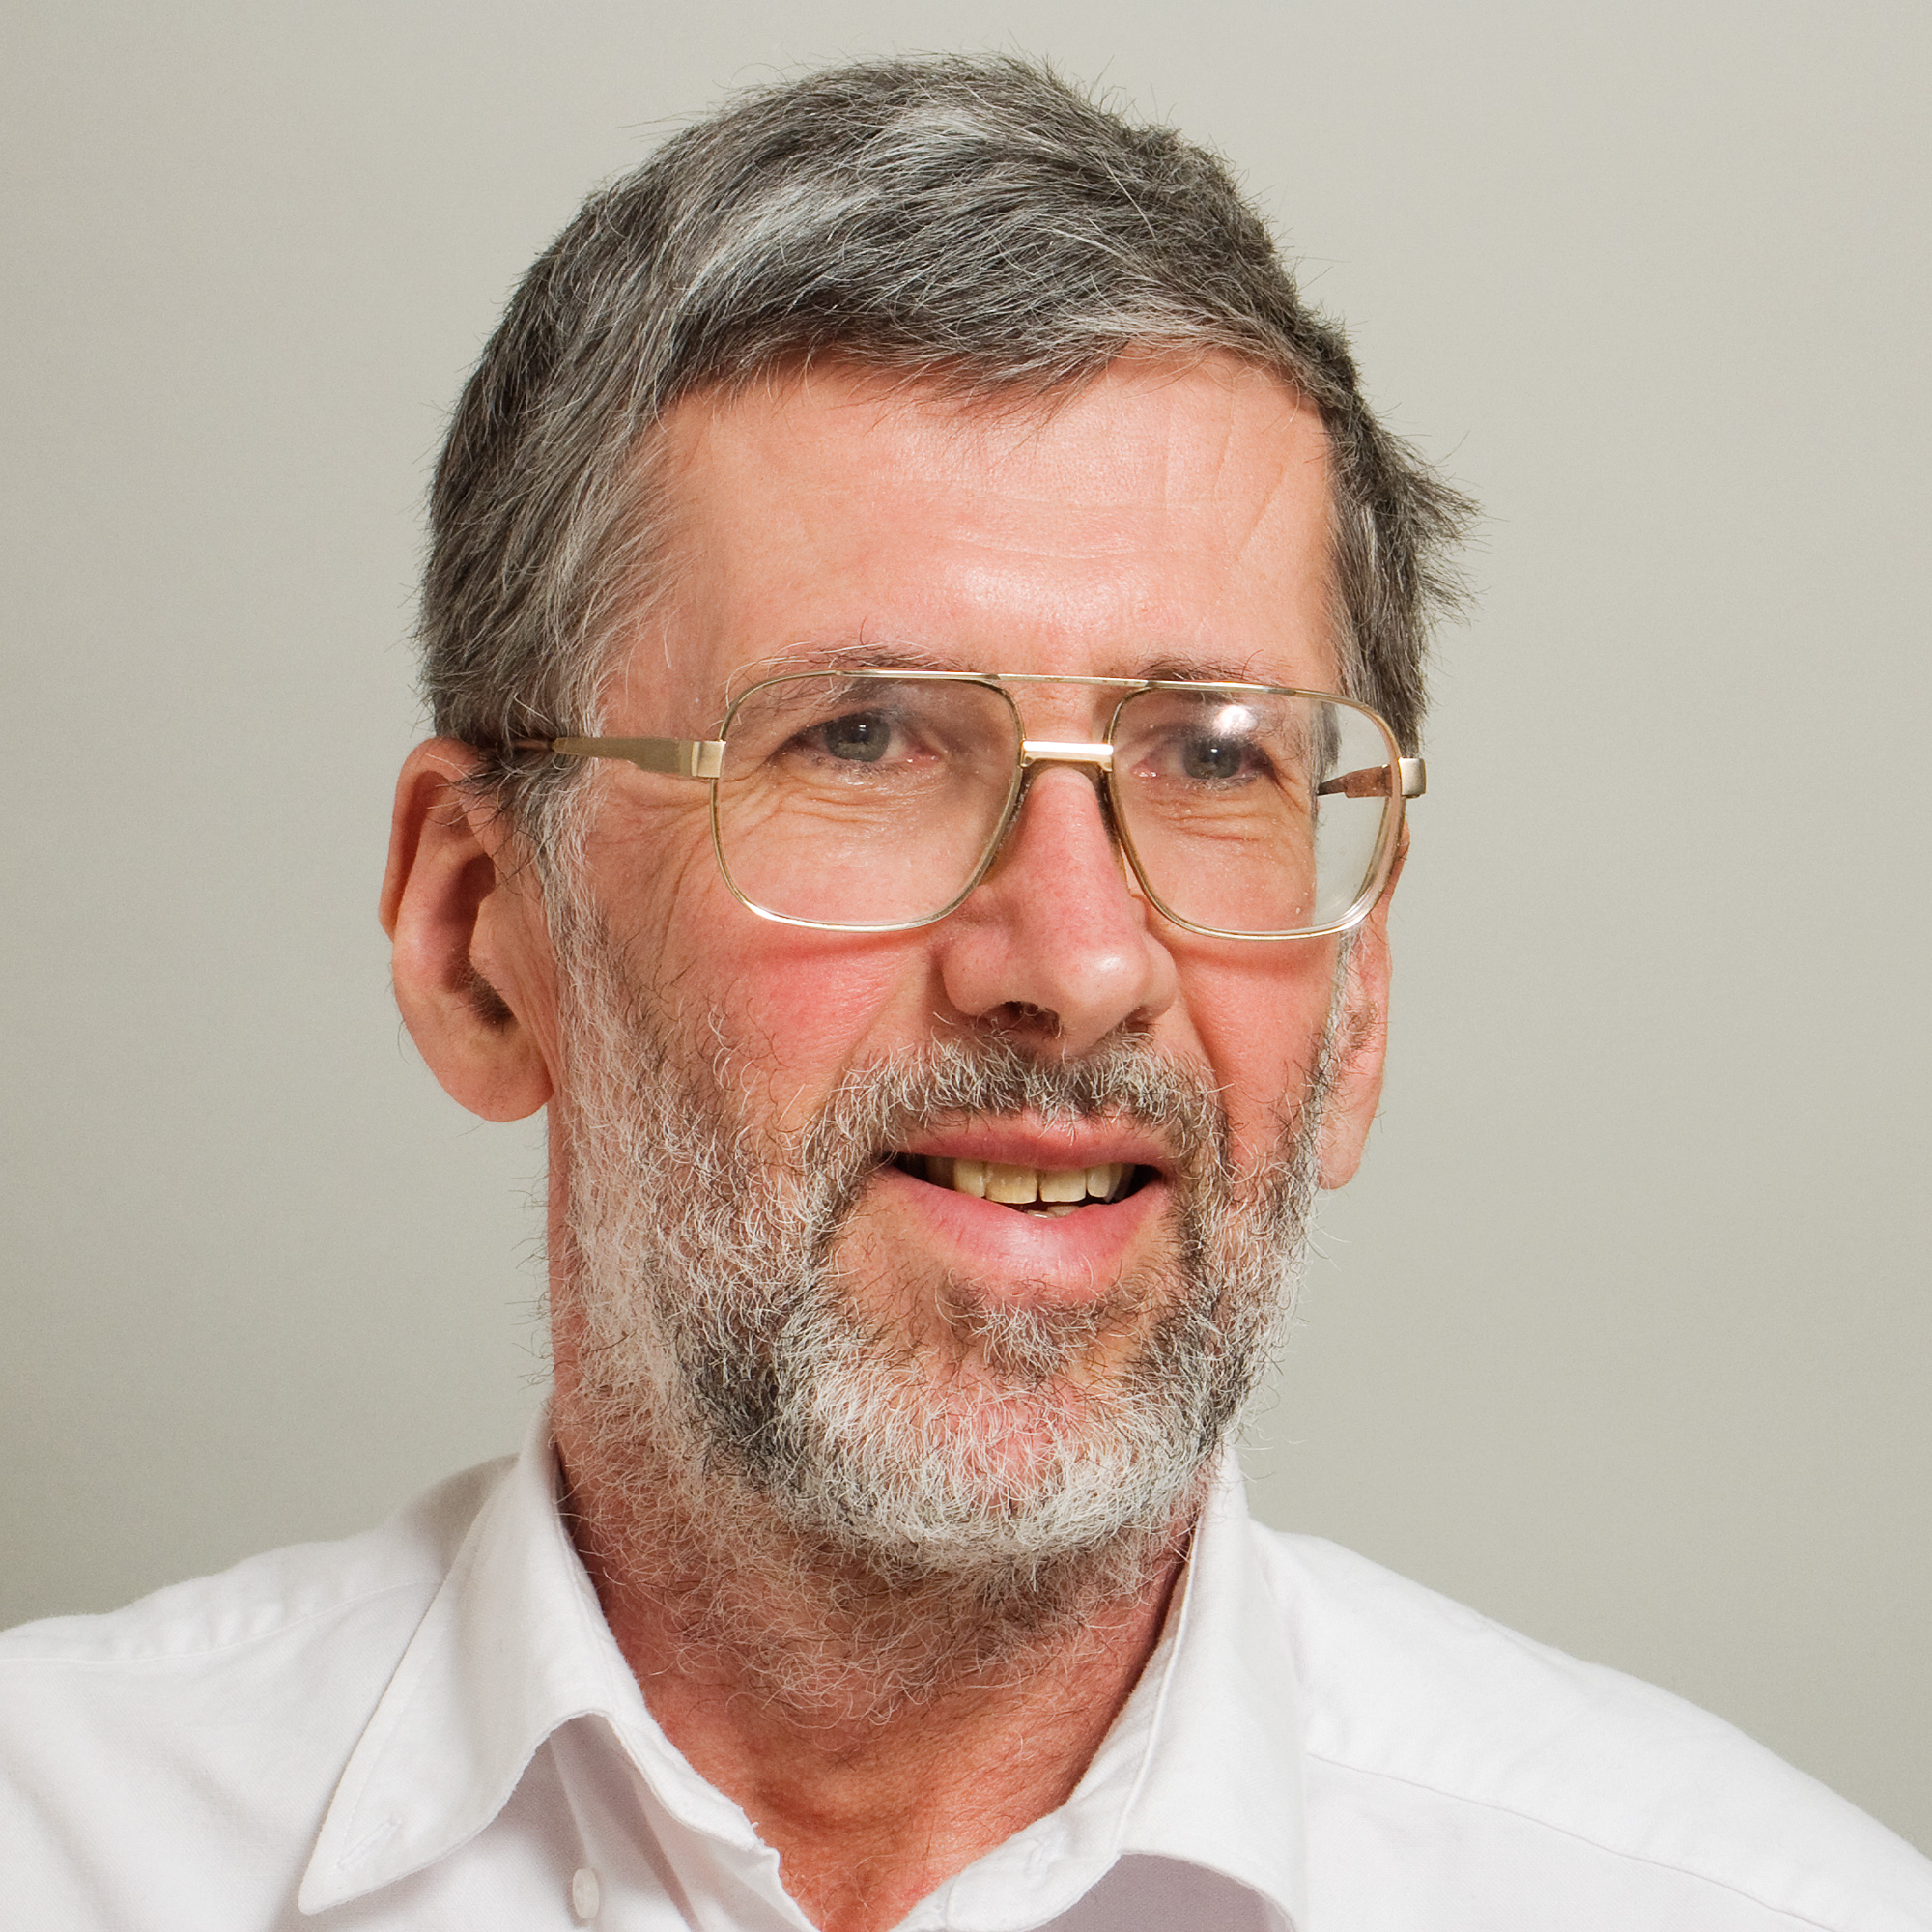
\includegraphics[width=0.4\textwidth]{Figures/reidar.jpg}
      \label{fig:partners_advisor_reidar}
\end{figure}
\textbf{Reidar Conradi}\\
Role: Professor at NTNU\\
Mobile: +47 91 89 70 29\\
Phone: +47 73 59 34 44\\
E-mail: conradi@idi.ntnu.no} & \parbox{7cm}{
Reidar Conradi was born in Oslo in 1946. He received his MS in 1970 and his Ph.D. in 1976, both from the Norwegian University of Science and Technology in Trondheim (NTNU), and has been at NTNU since 1975. He is now a professor at the Department of Computer and Information Science (IDI) at NTNU. His current research interests lie in software quality, software process improvement, version models, software evolution, component-based software engineering, open source software and related impacts, software engineering education, and associated empirical methods and studies. He is a member of ACM, IEEE, IFIP WG2.4 and ISERN.\cite{bioReidarConradi}
}
\end{tabular}
\label{tab:partners_advisor_reidar}
\end{table}

\subsubsection{Group}
\begin{table}[H]
\centering
\begin{tabular}{ p{7cm} p{7cm} }
\parbox{7cm}{
\begin{figure}[H]
      
\includegraphics[width=0.4\textwidth]{Figures/Person.png}
      \label{fig:partners_group_odd}
\end{figure}
\textbf{Odd Fredrik Rogstad}\\
Mobile: +47 99 10 73 27\\
E-mail: oddfredrikrogstad@gmail.com} & \parbox{7cm}{
Odd Fredrik was born in 1989 in Oslo. His family moved to Oppegård in 1990. He graduated from Oppegård VGS, today Roald Amundsen VGS, in 2008. From 2009 to 2010 he attended the mandatory military service, where he was based on Andøya military airbase in Andenes. He moved to Trondheim in 2010 and started his education at NTNU, where he started studying Computer Science, with specialization in Software Engineering. 

When he is not studying, he likes to work on smaller Android mobile application projects. Other interest are fishing, hunting, hiking, golf, computer games and cooking.
}
\end{tabular}
\label{tab:partners_group_odd}
\end{table}

\begin{table}[H]
\centering
\begin{tabular}{ p{7cm} p{7cm} }
\parbox{7cm}{
\begin{figure}[H]
      
\includegraphics[width=0.4\textwidth]{Figures/Person.png}
      \label{fig:partners_group_christian}
\end{figure}
\textbf{Christian Frøystad}\\
Mobile: +47 45 21 70 66\\
E-mail: chrisfro@stud.ntnu.no} & \parbox{7cm}{
Christian Frøystad was born in Fosnavåg in 1990. He graduated from Vestborg VGS (high school) in 2009. From 2009 to 2010 he studied theology at Fjellhaug Bibelskole.
In 2010, he started his education at NTNU, working towards a MS in Computer Science.

In 2008 he co-founded c, to become Xist AS in 2012.
He is also an active participant in the church Betania Misjonsforsamling, and a recreational musician.

His areas of interest includes theology, computer science, music, cooking, aviation, and general craftsmanship.
}
\end{tabular}
\label{tab:partners_group_christian}
\end{table}

\begin{table}[H]
\centering
\begin{tabular}{ p{7cm} p{7cm} }
\parbox{7cm}{
\begin{figure}[H]
      
\includegraphics[width=0.4\textwidth]{Figures/Person.png}
      \label{fig:partners_group_simon}
\end{figure}
\textbf{Simon Stastny}\\
Mobile: +47 45 16 62 98\\
E-mail: stastny.simon@gmail.com} & \parbox{7cm}{
    
Simon Stastny was born and brought up in Prague, Czech Republic.

He studied Software Engineering at the Czech Technical University, where he received his Bc in 2012. He now is a student of MSc in Information Systems at NTNU.

He has a background in backend development in Java-related technologies in his past and present occupations.

In his spare time, he is an avid bookworm, traveler, and CouchSurfer.

}
\end{tabular}
\label{tab:partners_group_simon}
\end{table}

\textbf{Knut Nergård}
\begin{table}[H]
\centering
\begin{tabular}{ p{7cm} p{7cm} }
\parbox{7cm}{
\begin{figure}[H]
      
\includegraphics[width=0.4\textwidth]{Figures/Person.png}
      \label{fig:partners_group_knut}
\end{figure}
\textbf{Knut Nergård}\\
Mobile: +47 41 25 67 20\\
E-mail: knut.nerga@gmail.com} & \parbox{7cm}{
Knut Nergård was born 1988 in Lærdal and moved shortly after to Hemsedal. He graduated from Gol VGS in 2007 and joined the army the following summer. From 2007 to 2008 he attended Forsvarets ingeniørhøgskole, and from 2008 to 2009 he went through the mandatory military service. In 2009, he started his education in Computer Science with specialization in Software Engineering. 

His interests entails music, programming, martial arts, cooking, computer games, bartending and knitting.
}
\end{tabular}
\label{tab:partners_group_knut}
\end{table}


\subsection{Background for the project}
Today, if you want information about cultural heritage you will have to access many different sources, and the information might be less than accessible. The joint European project TAG CLOUD aims to change this, and also bring together content provided by experts and individuals. TAG CLOUD is to develop innovative digital solutions to engage people in cultural heritage by making the information more accessible and involving the user in the content production.

In connection with this project eTrøndelag has decided, together with SINTEF ICT, to explore the possibility of using Virtual Walls to spread information about cultural heritage in Trondheim.

During the last 5 - 6 years, smart phones have become more and more common. In the later years mobile Internet has also become somewhat common. This has made this project possible, as the users do not need to carry an ordinary computer around.

\subsection{Project goal}
The goal of the project is to produce a prototype of the system that might be experimented with and tested in different contexts. The prototype should be accompanied by excellent documentation.

\section{Tools}
This section describes the tools used to communicate, develop and implement the system.

\subsection{Hardware \& development software}
As the system is to run on mobile phones, Android and iOS units was needed to perform tests along the way. The group has access to Android devices, but not iOS devices on a regular basis.

Titanium Studio\cite{titaniumStudio} is used while developing the mobile application. Titanium Studio is the official development environment from the creators of the framework Titanium.

\subsection{Collaboration and communication}
This section describes the tools used to collaborate and communicate throughout the project.

\subsubsection{Google Docs}
Google Docs\cite{googleDocs} is a freeware web-based office suite that enables multiple members to collaborate on documents, spreadsheets, presentations, drawings, etc. from any computer with Internet access. Google Docs uses Google Drive, which is a file storage and synchronization service. That means that two or more persons can work on the same document simultaneously, at different geographical locations. 

The group choses to use Google Docs because every group member has used it on previous projects. It is also fairly simple to use, so no training is needed. Since Google Docs has some limitations regarding appearance and navigation in documents, \LaTeX~will be used to produce the final document.

\subsubsection{\LaTeX}
\LaTeX~\cite{latex} is a document markup language and document preparation system for the \TeX~typesetting program. \LaTeX~enables the writer to make large, professional looking documents with table of content, placing of pictures and diagrams, cross-references, making tables, etc. taken care of by the software. 

Some group members have some experience with the markup language, but everyone else are eager to learn.

\subsubsection{Dropbox}
Dropbox\cite{dropbox} is a file hosting service that offers cloud storage and file synchronization, much like Google Drive. The group uses only Dropbox as an collaboration tool with the customer, as in sharing files, etc..

\subsubsection{Facebook}
Facebook is an online social networking service used by 1 110 million users worldwide\cite{facebook}. The group uses a private group, ``TDT4290 - CDP - Virtual Wall'', for everything from planning meetings, having scrum stand ups to discuss about the project.

\subsubsection{Email}
Email is used for communicating with both the customer and advisor. Within the group it is used for time sensitive matters, like changing meeting times.

\subsubsection{GitHub}
GitHub\cite{github} is a web-based hosting service for software development project that use the Git revision control system, which is a \gls{drcs}. Since Git is distributed every developer has their own local repository, independent of the centralized repository, this allows developers to work in offline mode and each of the local repositories acts as a backup. This was used during the implementation of the system.

\subsubsection{Trello}
Trello\cite{trello} is a free web-based project management application that uses the paradigm kanaban. Kanaban, a Japanese word that roughly mens ``card'' or ``signboard'', is a method made famous by the car manufacturer Toyota in the 1980s for supply management. 

Kanaban is fairly simple, a project is represented by a board, the board contains lists, that corresponds to a workflow. Lists contains cards that represents tasks.

\begin{figure}[H]
      \centering
      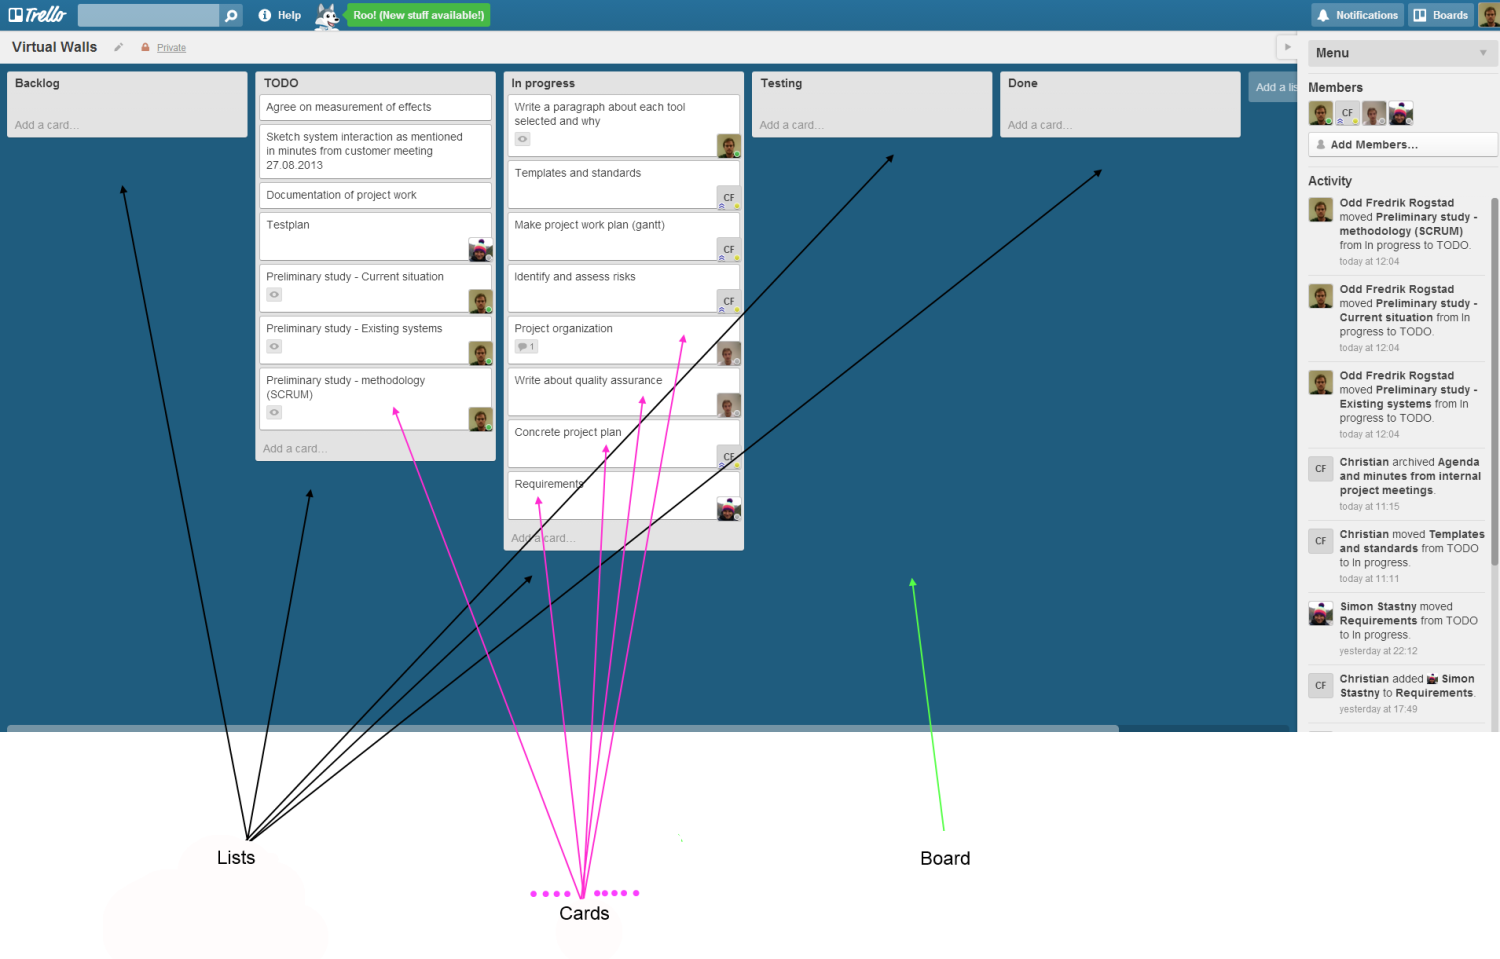
\includegraphics[width=0.8\textwidth]{Figures/trello.png}
      \caption{Screenshot of Trello}
      \label{fig:tools_trello}
\end{figure}

Figure~\ref{fig:tools_trello} shows how Trello is used for document work. There are several lists; ``TODO'', ``In Progress'', ``Testing'' and ``Done'', which represents the workflow. The process startes by populating the ``TODO''-list, with all the chapters needed. The group members then claims the different tasks, and starts working. When a person works on a task, then the corresponding card will be in the ``In progress'' list, when the task is finished, it is moved to the ``Testing'' list, for quality assurance. If it is approved, it will be moved to ``Done'' list, if not, back in the ``In Progress'' list.

\subsection{Allocated person-hours}
The course the project is part of amounts to 15 points of credit, which indicates that each member of the group should work for about 25 hours on the project each week. Given that the group consists of 4 members, and that the project run over 13 weeks, we get a total of allocated time that amounts to 25 hours per week per person x 4 persons x 13 weeks = 1300 hours.

Due to the diversity of the group, one in a full time job, the others attending different classes, the group has few meetings in person each week. As such, every group member is free to plan his own work each week, but has to meet at the weekly group meeting. As a result of this the group has only a few items on its weekly agenda: internal group meeting, meeting with advisor and meeting with customer.

\section{Detailed plan}
The goal of this chapter is to indicate how the project was executed. It was written as a guide on beforehand, but has been revised during the project lifetime in order to provide a better level of detail.

\subsection{Phases}\label{subsec:phases}
Here follows a short summary of the contents, duration and expected outcome of each phase.

\subsubsection{Planning and preliminary study}
Duration: 21.08.2013 - 11.09.2013 (3 weeks)\\
Expected outcome: Preliminary first chapters of report, requirements and test plan.

\subsubsection{Sprint 1}
Duration: 11.09.2013 - 25.09.2013 (2 weeks)\\
Expected outcome: Architectural documentation, refined requirements and test plan, and minimal working prototype. Complete phase document.

\subsubsection{Sprint 2}
Duration: 25.09.2013 - 09.10.2013 (2 weeks)\\
Expected outcome: Refined requirements and test plan, working prototype with developer documentation. Also complete phase document

\subsubsection{Sprint 3}
Duration: 09.10.2013 - 23.10.2013 (2 weeks)\\
Expected outcome: Refined requirements and test plan, working prototype with even better and more complete developer documentation. Complete phase document.

\subsubsection{Sprint 4}
Duration: 23.10.2013 - 13.11.2013 (3 weeks)\\
Expected outcome: Refined requirements and test plan, working prototype with excellent developer documentation.

\subsubsection{Finalization}
Duration: 06.11.2013 - 21.11.2013 (2 weeks)\\
Expected outcome: Excellent project report, presentation and prototype accompanied by user and developer documentation. Phase focuses primarily on finishing report and presentation, but also polishing the documentation.

\subsection{Activities}
Every week some meetings will take place.

\subsubsection{Customer meeting}
Each week a status is given, during the meeting, to the customer, as well as clarifying anything being unclear at that time. Backlog is prioritized every second week before the start of the next sprint.

\subsubsection{Advisor meeting}
This meeting is to report status and get valuable feedback and advice from the advisor.

\subsubsection{Internal group meeting}
This internal group meeting serves as the planning meeting for the coming week.

\subsection{Milestones}

\subsubsection{Pre-delivery of report}
Due: 14.10.2013\\
Delivery of the chapters Abstract, Introduction, Pre-study and the one containing choice of development model. The outline of the report should also be finalized in the table of contents. The outline does not need to be complete, but should give a good indication as to what each sections is to discuss.

\subsubsection{Production of reports}
Due: 20.11.2013\\
The report is to be copied and bound in four copies no later than 20.11.2013. Preferably earlier.

\subsubsection{Final delivery and presentation}
Due: 21.11.2013\\
Presentation for customer, advisor and censor. After the presentation, a copy of the report should be given to the customer and three copies should be delivered to the information desk at IDI. A PDF version should also be sent by email to anreala@idi.ntnu.no.

All copies is to be accompanied with a CD that contain the implementation, documentation and a PDF version of the report. The content of this CD will be documented with a ``Readme.txt'' file, as specified in the compendium.

\subsection{Gantt diagram}
\begin{figure}[H]
      \centering
      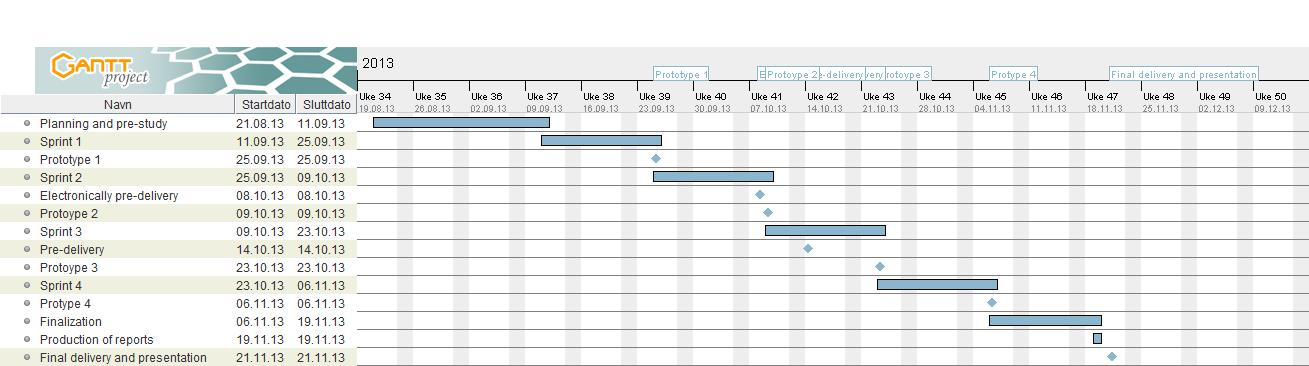
\includegraphics[width=0.4\textwidth]{Figures/gantt.jpg}
      \caption{Overview of project}
      \label{fig:plan_gantt}
\end{figure}

\begin{table}[H]
\centering
\begin{tabular}{ l | r r r r r r }
    Activity               & Planning    & Sprint 1  & Sprint 2  & Sprint 3  & Sprint 4  & Finalization    \\ \hline        
    Lectures                & 60        & 4         & 4         & 4         & 4         & 4               \\ \hline
    Admin                   & 25        & 20        & 20        & 20        & 20        & 50              \\ \hline
    Planning                & 50        & 8         & 8         & 8         & 8         & 50              \\ \hline
    Pre-Study               & 100       & 20        & 20        & 10        & 10        & 10              \\ \hline
    Requirements            & 60        & 15        & 15        & 10        & 10        & 0               \\ \hline
    Design                  & 5         & 30        & 30        & 15        & 15        & 0               \\ \hline
    Implementation          & 0         & 60        & 60        & 50        & 50        & 10              \\ \hline
    Testing                 & 0         & 22        & 22        & 50        & 50        & 38              \\ \hline
    Documentation           & 0         & 21        & 21        & 33        & 33        & 38              \\ \hline
    Sum                     & 300       & 200       & 200       & 200       & 200       & 200
\end{tabular}
\caption{Time sheet per phase}
\label{tab:plan_time_per_phase}
\end{table}

\section{Risks}\label{sec:project_risk_assessment}

\begin{table}[H]
\centering
\begin{tabular}{ l  p{11cm} }
    Id                      & R1                                                                          \\ \hline
    Activity                & All activities                                                              \\ \hline
    Risk factor             & Group member having a full time job in addition to being 75 \% student      \\ \hline
    Consequences            & H: The quality and scope of the project might suffer                        \\ \hline
    Probability             & M                                                                           \\ \hline
    Strategy and actions    & Monitor situation closely. Have clear assignments and agreements                 \\ \hline
    Deadline                & Continuously                                                                \\ \hline
    Responsible             & Project leader                                                              \\ 
\end{tabular}
\caption{R1: Group member not having time to prioritize the project}
\label{tab:risk_1}
\end{table}

\begin{table}[H]
\centering
\begin{tabular}{ l  p{11cm} }
    Id                      & R2                                                                          \\ \hline
    Activity                & All activities                                                              \\ \hline
    Risk factor             & Getting sick                                                                     \\ \hline
    Consequences            & H: The available work power might be reduced and tasks delayed.             \\ \hline
    Probability             & M                                                                           \\ \hline
    Strategy and actions    & All tasks to be entered into task management system. 
                              When sick, the group should be informed and if necessary tasks assigned.    \\ \hline
    Deadline                & Continuously                                                                \\ \hline
    Responsible             & Everyone\\
\end{tabular}
\caption{R2: Group member getting sick}
\label{tab:risk_2}
\end{table}

\begin{table}[H]
\centering
\begin{tabular}{ l  p{11cm} }
    Id                      & R3                                                                          \\ \hline
    Activity                & All activities                                                              \\ \hline
    Risk factor             & Lack of responsibility                                                      \\ \hline
    Consequences            & H: Other members must do the work originally assigned to some other member  \\ \hline
    Probability             & M                                                                           \\ \hline
    Strategy and actions    & Make understandable tasks with clear deadlines. Other members might take 
                                some of the workload, stalling other parts of the project. If need be, 
                                the course staff should be notified.                                      \\ \hline
    Deadline                & Continuously                                                                \\ \hline
    Responsible             & Everyone                                                                    \\ 
\end{tabular}
\caption{R3: Lack of responsibility}
\label{tab:risk_3}
\end{table}

\begin{table}[H]
\centering
\begin{tabular}{ l  p{11cm} }
    Id                      & R4                                                                          \\ \hline
    Activity                & Cooperation                                                                 \\ \hline
    Risk factor             & Internal conflicts                                                          \\ \hline
    Consequences            & M: As the social environment will suffer, it will drain more energy from 
                                the people involved. This will in turn most likely reduce quality of 
                                the work done.                                                            \\ \hline
    Probability             & M                                                                           \\ \hline
    Strategy and actions    & Resolve disagreements before they turn into conflicts and respect that 
                              others might have a different opinion.                                      \\ \hline
    Deadline                & Continuously                                                                \\ \hline
    Responsible             & Everyone                                                                    \\ 
\end{tabular}
\caption{R4: Internal conflicts}
\label{tab:risk_4}
\end{table}

\begin{table}[H]
\centering
\begin{tabular}{ l  p{11cm} }
    Id                      & R5                                                                          \\ \hline
    Activity                & Communication with customer                                                 \\ \hline
    Risk factor             & Miscommunication                                                            \\ \hline
    Consequences            & H: The solution delivered might not be the solution asked for               \\ \hline
    Probability             & M                                                                           \\ \hline
    Strategy and actions    & Keep regularly and often in touch with customer. Write minutes, and get 
                              them approved by customer. Work in increments, and demo the current 
                              state of the prototype often.                                               \\ \hline
    Deadline                & Continuously                                                                \\ \hline
    Responsible             & Customer contact and secretary                                              \\ 
\end{tabular}
\caption{R5: Miscommunication}
\label{tab:risk_5}
\end{table}

\begin{table}[H]
\centering
\begin{tabular}{ l  p{11cm} }
    Id                      & R6                                                                          \\ \hline
    Activity                & Collaboration                                                               \\ \hline
    Risk factor             & Distributed work                                                            \\ \hline
    Consequences            & H: Efficiency might lower and quality could be reduced                                 \\ \hline
    Probability             & M                                                                           \\ \hline
    Strategy and actions    & Daily updates on the current work. Check each others work. Tasks with 
                              clear deadlines                                                             \\ \hline
    Deadline                & Continuously                                                                \\ \hline
    Responsible             & Everyone                                                                    \\ 
\end{tabular}
\caption{R6: Distributed work}
\label{tab:risk_6}
\end{table}

\section{Project organization}
The following section describes how the team was structured in the project. We go through what roles team members are allocated to, what the roles entails.

\begin{table}[H]
\centering
    \begin{tabular}{ l  p{11cm}  }
    Role                    & Member                                                                      \\ \hline
    Customer contact        & Odd Fredrik Mørch Rogstad                                                   \\ \hline
    Scrum master            & Odd Fredrik Mørch Rogstad                                                   \\ \hline
    Secretary               & Christian Frøystad                                                          \\ \hline
    Test leader             & Simon Stastny                                                               \\ \hline
    Project manager         & Knut Nergård                                                                \\
\end{tabular}
\caption{Group organization}
\label{tab:org}
\end{table}

Following, we list the different roles in the team, and what the tasks that comes with the positions is. This is to be seen as guidelines, the individuals are not necessarily expected to do all the work related to the position by themselves. They are however responsible for making sure it is being done.

\subsection{Customer contact}
The customer contact is responsible for the activities involving the customer. He is to arrange meetings with customer, keep the customer informed and generally serve as the contact person for the team in regards to the customer.

\subsection{Scrum master}
The scrum master is responsible for making sure the sprints progress as planned. If needed he will make alterations to the plans to better fit the current status.

\subsection{Secretary}
The main responsibility for the secretary is to get what is being discussed down in writing. He takes notes during the meetings the team attends, and writes minutes of the meetings which is then distributed to the team .

\subsection{Test leader}
The test leader is responsible for the activities around testing. This includes the writing of tests, ensuring that they cover the requirements the customer has set, the execution of tests, and handling the results from the tests, figuring out what has to be done as a result of the test.

\subsection{Project manager}
The project manager is responsible for keeping the project on track. He should know the status of the project at any time, and know what has to be done to make progress. He ensures that everyone in the team has something to do and keeps track of the hours spent from the individuals in the team. Finally he is responsible for keeping a positive work environment in the team, working to solve conflicts if they may arise.

\section{Quality Assurance}
Quality assurance is an important part of any project. Without any sort of standards and routines, the collaboration of the group will suffer major setbacks once you need to combine the individual works in the group to the final product, as well as general confusion and/or uncertainty. To ensure our product turns out the best possible way and that the organization was pleasing, we started early setting up rules for communication within the group as well as external communication with customer and supervisor. Routines of the method of work was set up, and standardized templates were created.

\subsection{Routines}
Having a group with widely different time schedules, we quickly figured out that a more decentralized work structure would be in order. By doing this, we further increased the importance of good routines for work sharing and communication, as the group meetings were scarce and errors or misunderstandings might exist for a prolonged time if they first surfaced.

\subsubsection{For work sharing}
To handle sharing of individual works, a shared google disk was used. The access was only given to the group members, as this was not the platform we used to share files with the customer and advisor. The google disk was structured into several subfolders. Any document that is to be shared with externals, that being customer or advisor, is first stored in the respective customer and advisor folders, edited if needed, and approved by the group before they are sent to the externals in the selected way of communication. Files to be shared within the group had it's own folders as well. Lastly, each member has a private folder to note down hours spent or to store files not ready to be fully shared yet.

To share documents with externals, the group has taken use of dropbox and mail. Documents that has been approved by the group is sent either by mail or added to the shared dropbox folder where the externals can access them.

\subsubsection{For communication}
To create a good channel for communication within the group and externally, several steps were taken. Our main communication tool internally was a facebook project group. Here, internal messages, meeting reminders, questions and answers with more was posted. We also agreed using a mailing list in addition for more short-time updates, like meetings being canceled. This was seen as a necessary step after an unfortunate experience were not everyone noticed the cancellation message in time.

\subsubsection{For group meetings}
Even though our system of working in separate locations works to a certain degree, we still needed some meetings to make sure the group was somewhat synchronized and kept on the right track both according to the customer as well as internal work.

To manage this we set up meetings for the group. Once a week, we arranged a customer meeting, an advisor meeting and a group meeting.

\subsection{Customer meeting}
We held weekly meetings with the customer. The meeting day and time was scheduled on a weekly basis, and more or less bound to Tuesdays or Wednesdays. The goal with these meetings was to establish a common understanding on how the system should be, and find the right requirements to agree upon. To make sure we are in an understanding with the customer, we take notes and create minutes from the meeting. This is in turn sent back to the customer, who either approves them or brings back feedback on what was misunderstood for the next weeks meeting. If anything happened to be misunderstood, this will be detected and changed within a week, preventing major workloads on the wrong premise. In addition to the minutes, we used action points, which are activities the customer wants us to look into or complete before the next meeting. This could be creating time estimates of user tests, architecture overviews, UI suggestions and more.

\subsection{Advisor project meeting}
Once a week, we met with the advisor to discuss how the project was coming along. If the team faced any problems with the project or the team which we could not manage solving by ourselves, this was the place to get assistance. This could be anything from lack of required knowledge to personal conflicts within the team. The meetings were also held to give the advisor an overview of our situation. Weekly status reports and timesheets were given to help the advisor keeping an overview of the progress of the project.

\subsection{Internal group meeting}
At least once a week, we held group meetings. The goal with these meetings was to help synchronizing the group, updating all the members on what was done and what was to be done, raise important questions about further progress, or simply having a place to raise questions or concerns that does not fit other places. Although we simultaneously used a shared document where the team members wrote their progress and intended actions, the meetings ensured everyone was being a part of the update. Important decisions also benefited from having all team members come together on a solution, so no one feels left out of the process as well as smart solutions that otherwise might be overlooked is included.  In that regard, group meetings were held when as many as possible could attend.

\section{Templates and procedures}
Here the established standards are outlined.

\subsection{Document templates}
The group has established standard documents for agendas for meetings with respectively the customer, the advisor and the group. A template has also been made for writing minutes from each meeting.

A template for the weekly status report has also been made, and can be used with few modifications every week.

For meeting invitations a standard has also been established so that inviting people to meetings should be done in an uniform way and as effectively as possible.

\subsection{Code standards}
See section ~\ref{sec:codeStandard} for complete code standards for both the server and the client.

\subsection{Version control procedures}
All documents are produced in Google Docs, which incorporates version control for each document. The documents will regularly be backed up on local storage.

All code will be tracked with git and checked in continuously in order to always be consistent.

\chapter{Preliminary study}
\label{chap:preliminary_study}

\section{Current situation}
Cultural Heritage is the legacy of physical artifacts and non physical attributes of a group or society that are inherited from past generations. According to \cite{CiD:culturalheritage}, cultural Heritage can be divided into three main categories; tangible culture, intangible culture and natural heritage. The system will mainly focus on the ``culture in the landscape'', i.e. the discovery of cultural memories that we meet when walking around in cities, in villages and in the nature.

An important aspect in cultural heritage is preservation, the task to preserve and protect buildings, objects, landscapes and other important cultural artifacts. One thing is to physically protect these artifacts, but another important aspect is to educate today's generation and help them discover and learn about our cultural heritage to both enrich and preserve our legacy for future generations.

This section will give the reader a better understanding of the current situation in how cultural heritage is preserved today. It will also take a look at existing mobile applications that helps people discover and learn about cultural heritage.

\subsection{Cultural Heritage today}
The most famous organization working with cultural heritage is UNESCO \cite{UNESCO:intro}. The United Nations Education, Scientific and Cultural Organization is an agency of the UN (United Nations), working for peace and security through international collaboration in education, science and culture. UNESCO World Heritage Committee is responsible for establishing  the famous list of UNESCO World Heritage Sights \cite{UNESCO:worldheritage}, which today contains 981 properties (September 2013), that includes cultural, natural and mixed properties.

There are seven listings in Norway that the UNESCO World Heritage Committee consider having outstanding universal value, that is;

\begin{enumerate}
  \item Bryggen, Bergen, Hordaland
  \item Urnes Stave Church, Luster, Sogn and Fjordane
  \item Røros Mining Town and the Circumference, Røros, Sør-Trøndelag
  \item Rock Art of Alta, Alta, Finnmark
  \item Vegaøyan -- The Vega Archipelago, Vega, Helgeland
  \item Struve Geodetic Arc, multiple measuring points in several countries
  \item West Norwegian Fjords - Geiranger and Nærøyfjord, Møre and Romsdal, and Sogn and Fjordane
\end{enumerate}

These are really marvelous pieces of cultural heritage, but is that it? Does Norway have only seven sights that are considered as cultural heritage and worth a visit? Of course not, our scope is much broader than that. It is up to the users to decide what cultural heritage is.

\subsection{Existing systems}
In 2004 The Directorate for Cultural Heritage in Norway (Riksantikvaren) launched a database, called Askeladden, over protected cultural heritage sights and cultural environments in Norway. The problem was that it was only available to agencies involved in cultural heritage management, and not to the public. However,  in 2009, parts of the database was finally made available through the website Kulturminnesøk (kulturminnesok.no), and today, after a bigger upgrade in 2012, it contains over 150 000 sights.

\begin{figure}[H]
      \centering
      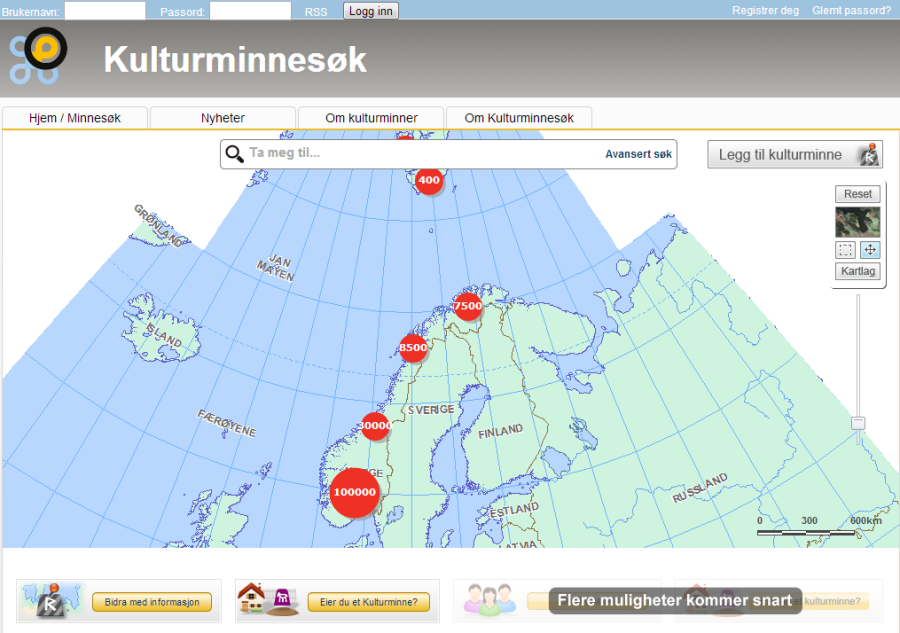
\includegraphics[width=0.8\textwidth]{Figures/Prestudy/kulturminnesokOversikt.png}
      \caption{Kulturminnesøk, Norway}
      \label{fig:pre_kulturoversikt}
\end{figure}

\begin{figure}[H]
      \centering
      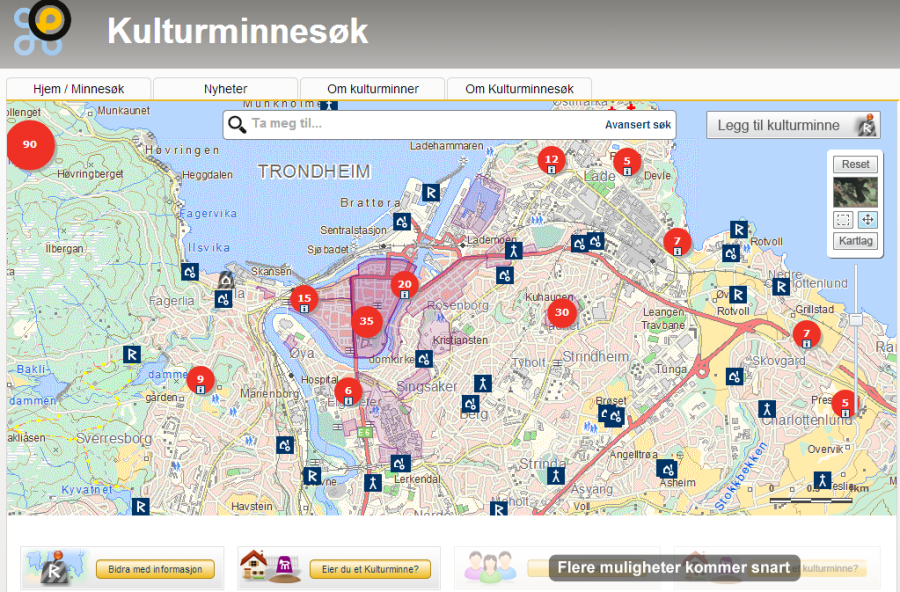
\includegraphics[width=0.8\textwidth]{Figures/Prestudy/kulturminnesokTrondheim.png}
      \caption{Kulturminnesøk, Trondheim}
      \label{fig:pre_kulturTrondheim}
\end{figure}

As you can see in Figure~\ref{fig:pre_kulturoversikt}, sights from all over Norway are represented. We can either press the red circles, zoom in manually or search by text to find places we want to take a closer look at. If we zoom in over Trondheim, as Figure~\ref{fig:pre_kulturTrondheim} shows, there are plenty of sights all over the city. Every sight is marked with a symbol, which tells the user if it is a building location, religious place, archaeological memory or technical/industrial memory. If you click on a symbol, a small info display appears, Figure~\ref{fig:pre_kulturInfo}, that informs the user what type of cultural heritage it is, its conservation status, dating and municipality. If the user wants more info, the user can press the ``Mer info'' (More info)-text, and  a new sight appears, Figure~\ref{fig:pre_kulturMoreInfo}, where a picture, if available, and a some more info appears. It is also possible to comment and like (as in Facebook) the site.

\begin{figure}[H]
      \centering
      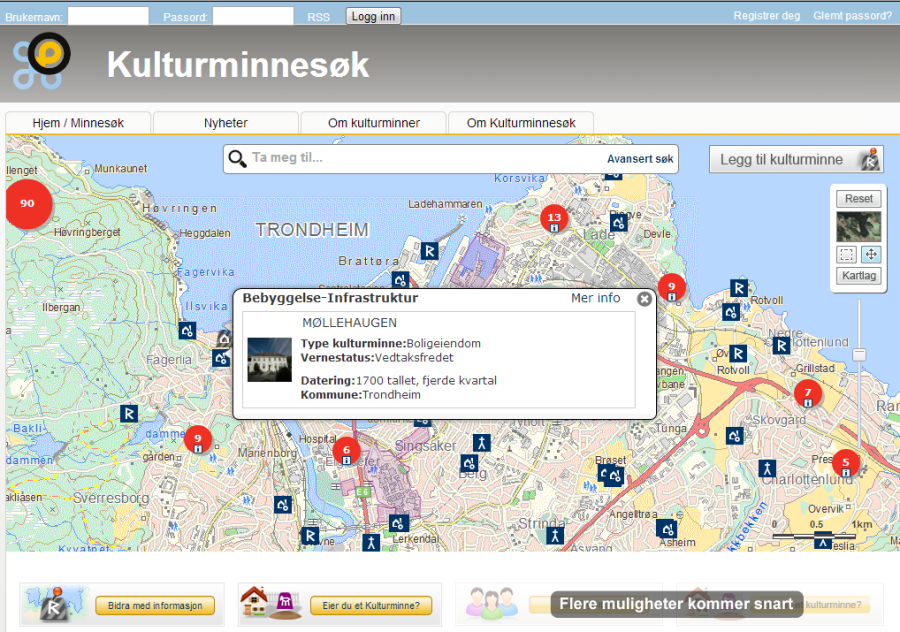
\includegraphics[width=0.8\textwidth]{Figures/Prestudy/kulturminnesokClick.png}
      \caption{Kulturminnesøk, info display}
      \label{fig:pre_kulturInfo}
\end{figure}

\begin{figure}[H]
      \centering
      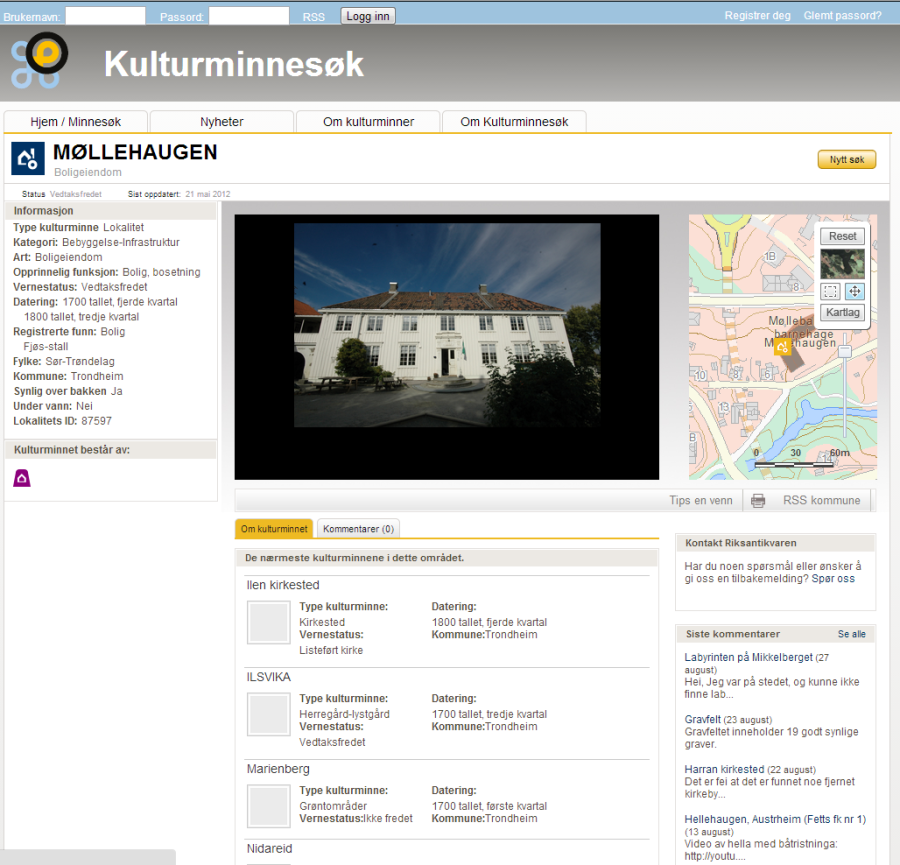
\includegraphics[width=0.7\textwidth]{Figures/Prestudy/kulturminnesokMoreInfo.png}
      \caption{Kulturminnesøk, more info}
      \label{fig:pre_kulturMoreInfo}
\end{figure}

Kulturminnesøk can be considered a partly edge dominant system\footnote{the term edge dominant system is explained in section~\ref{subsec:edge}}, since everyone can register and add their own cultural heritage sight. There is about 1500 sights that users have added. Users have added everything from swimming halls to archaeological memories. We call it just partly edge dominant, since only 1\% of the content is added by the public.

\begin{figure}[H]
      \centering
      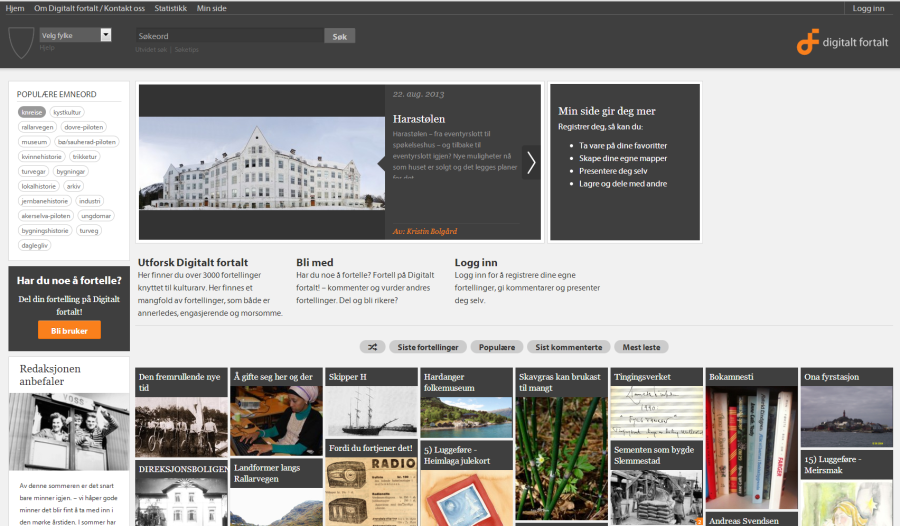
\includegraphics[width=0.8\textwidth]{Figures/Prestudy/digitaltfortaltForside.png}
      \caption{Digitalt fortalt, front page}
      \label{fig:pre_fortaltFrontPage}
\end{figure}

Another edge dominant cultural heritage system is ``Digitalt fortalt'' (norwegian for ``digitally told''). Digitalt Fortalt is a website where users, cultural institutions or private persons can register and add stories related to cultural heritage. Users have added stories about everything from clothespins to protected buildings, and today there are over 3000 stories. 

To read a story you can either search, by pressing one of the popular tags or simply search from the search field, or browse on the front page, in last told stories, popular stories, last commented stories or among the most  read stories. If we search on ``Trondheim'' in the search field, we get 135 hits. The stories are placed in a grid system, and every story is represented in a little box, with a title, a picture (a play-sign if a sound is attached to the story), author and location. Some stories are also linked to a date or a period. The search result is shown in Figure~\ref{fig:pre_fortaltTrondheim}.

If we press one of the stories, Regalierommet for instance, shown in Figure~\ref{fig:pre_fortaltRegalierommet}, a page with a media slider and information appears. In this case the story is represented as sound and pictures. The information below the media slider says something about why it was made, and some information about the creators. In other stories there are typically one or more pictures and the story represented with text.

\begin{figure}[H]
      \centering
      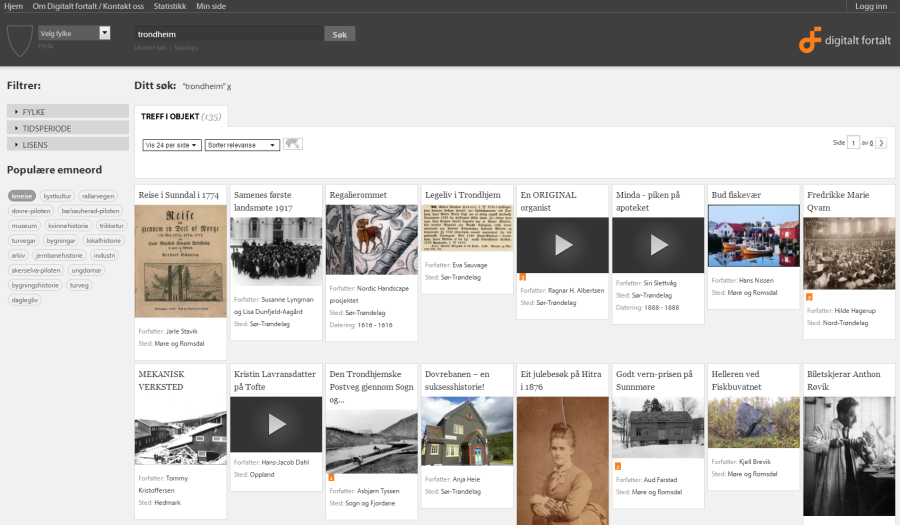
\includegraphics[width=0.8\textwidth]{Figures/Prestudy/digitaltfortaltSokTrondheim.png}
      \caption{ Digitalt fortalt, search result for Trondheim}
      \label{fig:pre_fortaltTrondheim}
\end{figure}

\begin{figure}[H]
      \centering
      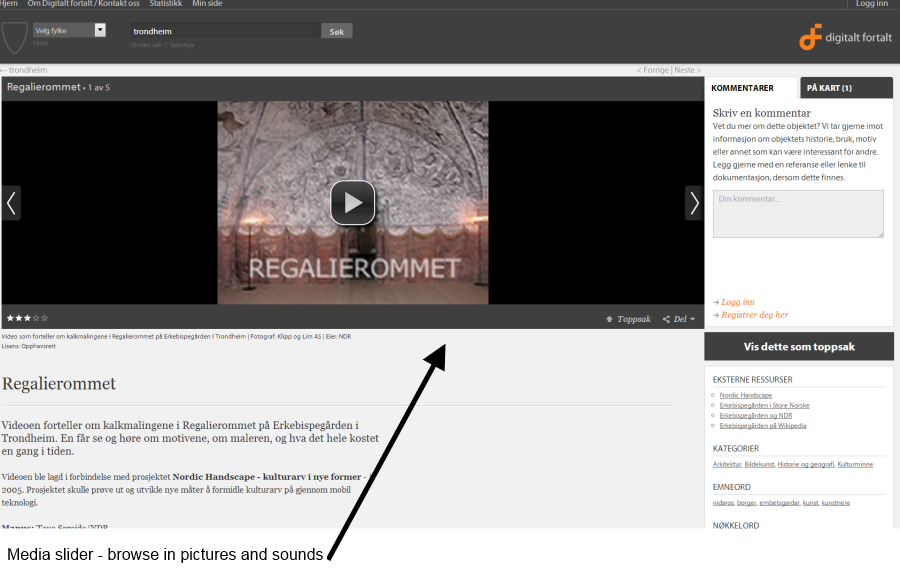
\includegraphics[width=0.8\textwidth]{Figures/Prestudy/digitaltfortaltRegalierommet.png}
      \caption{Digitalt fortalt, Regalierommet, with media slider and text}
      \label{fig:pre_fortaltRegalierommet}
\end{figure}

\subsection{Edge dominant systems}\label{subsec:edge}
An edge dominant system is one that almost entirely depends on input from users. Well known edge dominant systems today are Facebook, Twitter, YouTube, Wikipedia, etc., all of which have created enormous value by their users. 

Almost all edge dominant systems today share a common ecosystem structure, called a ``Metropolis'' structure, by analogy with a city, as shown in Figure~\ref{fig:pre_edgeMetropolis}.

\begin{figure}[H]
      \centering
      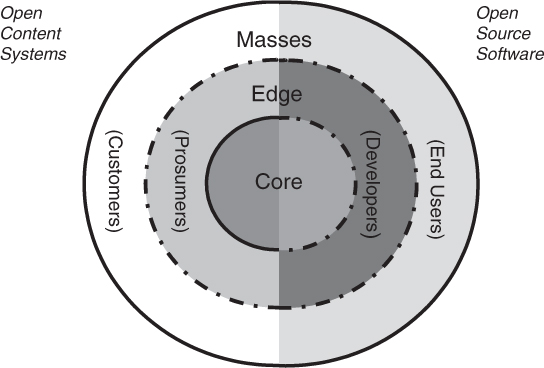
\includegraphics[width=0.8\textwidth]{Figures/Prestudy/metropolis.jpg}
      \caption{The metropolis}
      \label{fig:pre_edgeMetropolis}
\end{figure}

The metropolis structure divides the communities of stakeholders in an edge dominant system:

\begin{itemize}
  \item The outermost ring consists of the masses: customers and end users. They consume the content made by the metropolis, and contribute requirements.
  \item The middle ring contains prosumers and developers. These are the people that produces the content for the metropolis. The developers write software for the community to use, and the prosumers produce (and consume) content in the metropolis.
  \item The center ring is the core that keeps the metropolis together. This is the software that provides its services through a set of APIs that the prosumers and developers can use to produce new software and content for the masses to use.
\end{itemize}

\section{Existing mobile applications}\label{sec:prestudy_existing_apps}
In the previous sections we have learned that there already are systems that help the public in finding cultural heritage. In this section we will look at some existing mobile applications which in many ways works quite similar to the systems above. It is important to look at these systems to get an idea of how others have done it before us, both to get inspired and to find weaknesses with this kind of applications. First we will take a look at Kulturminnesøk's mobile application, then at two Danish solutions.

\subsection{Kulturminnesøk app}
After using Kultruminnesøk in the web browser we discovered that they also had a mobile application. Not surprisingly, the mobile application serves much of the same functions as the web application, and has certain drawbacks and  advantages. First of all, it has the same map function, Figure~\ref{fig:pre_kulturMinneAppMap}, you can zoom in and out with the well known ``pinch-to-zoom'' gesture, which allows the user to zoom in or out by moving two fingers further apart or closer together while touching the display. The same symbols as in the web application is used, and we can press them to get more information. In addition to the map you can use a list function where you can see your nearest sights, Figure~\ref{fig:pre_kulturMinneAppList}. However, the coolest function is the mobile application is in the function ``Vis meg'', or ``Show me''; this is a augmented reality function, where all sights within a certain range appears on the screen, through a camera application, represented by the same symbols in the map, Figure~\ref{fig:pre_kulturMinneAppAug}.  A quite significant drawback is that there are no pictures in the ``More info'' display, but the biggest weakness is that the application does not show user-created sights, just the cultural sights from the Askeladden database.

\begin{figure}[H]
      \centering
      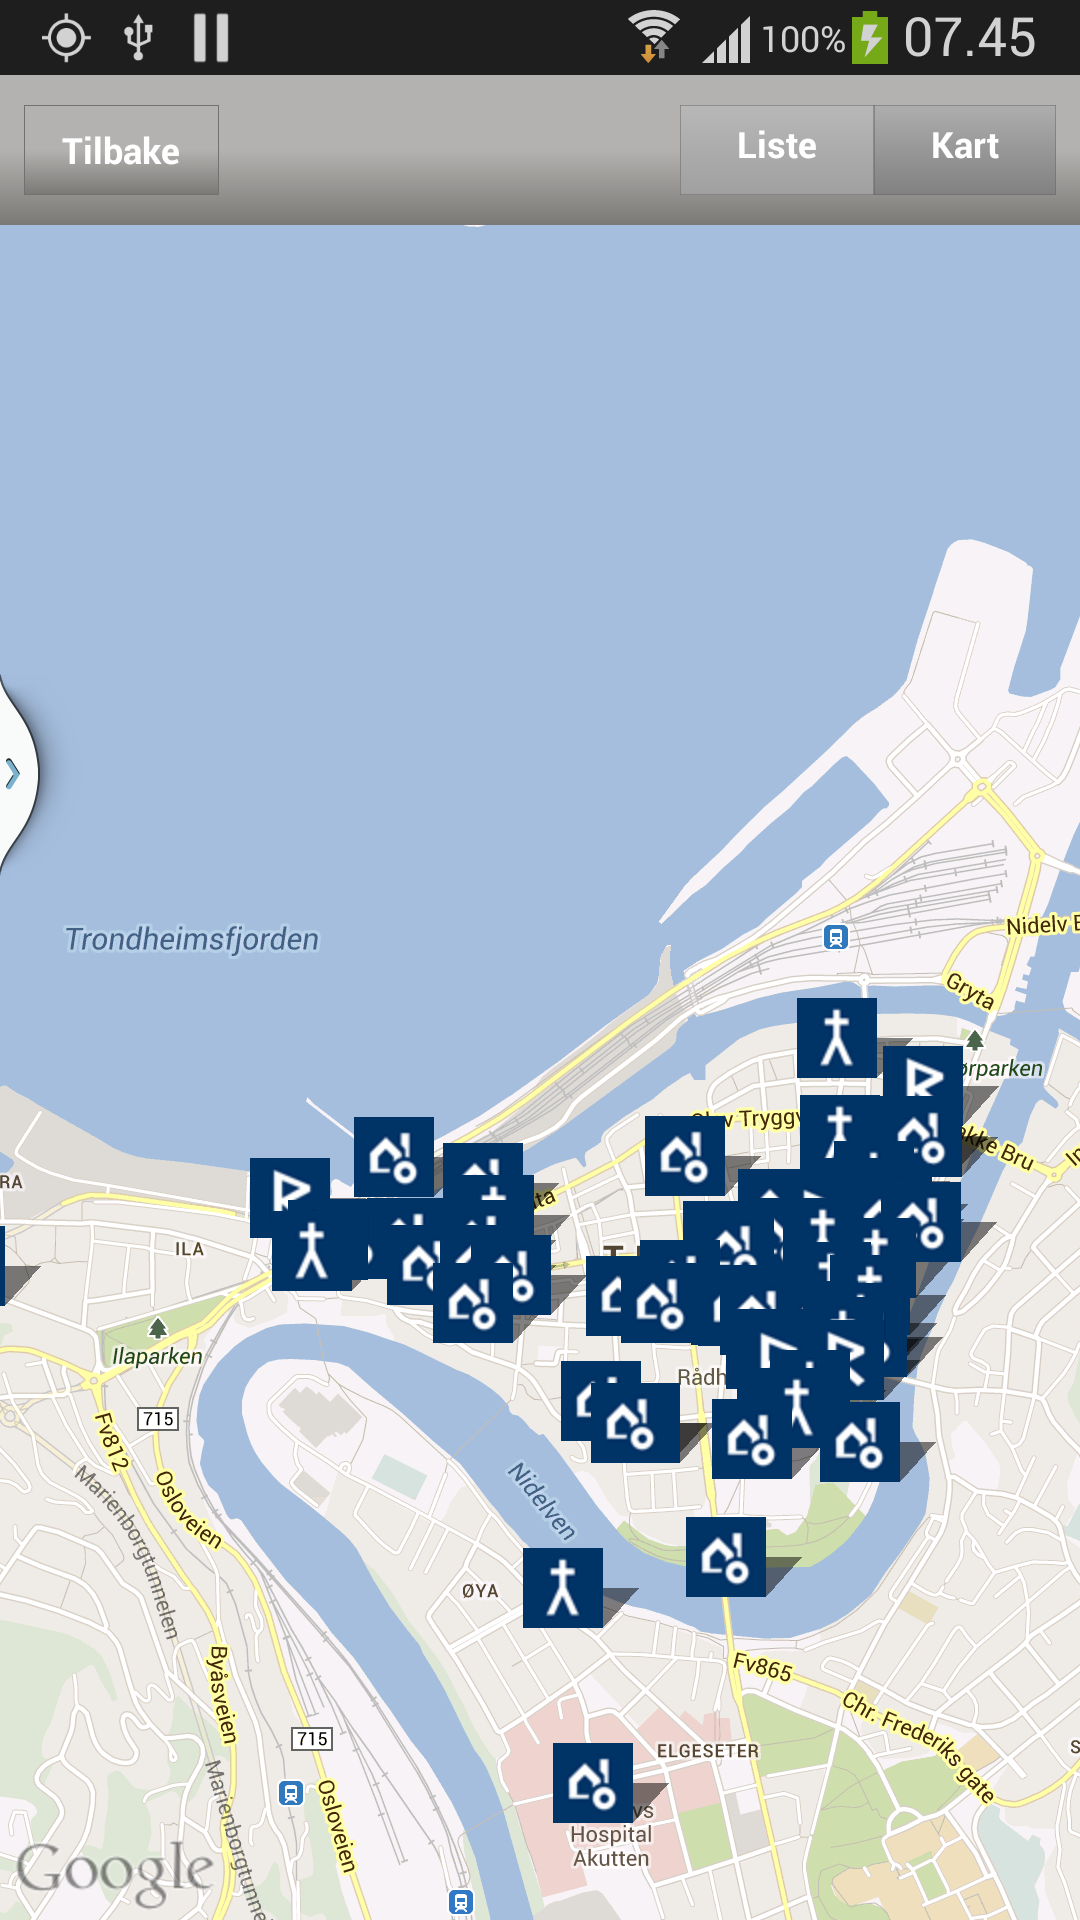
\includegraphics[width=0.4\textwidth]{Figures/Prestudy/kulturSokMap.png}
      \caption{Kulturminnesøk, map function}
      \label{fig:pre_kulturMinneAppMap}
\end{figure}

\begin{figure}[H]
      \centering
      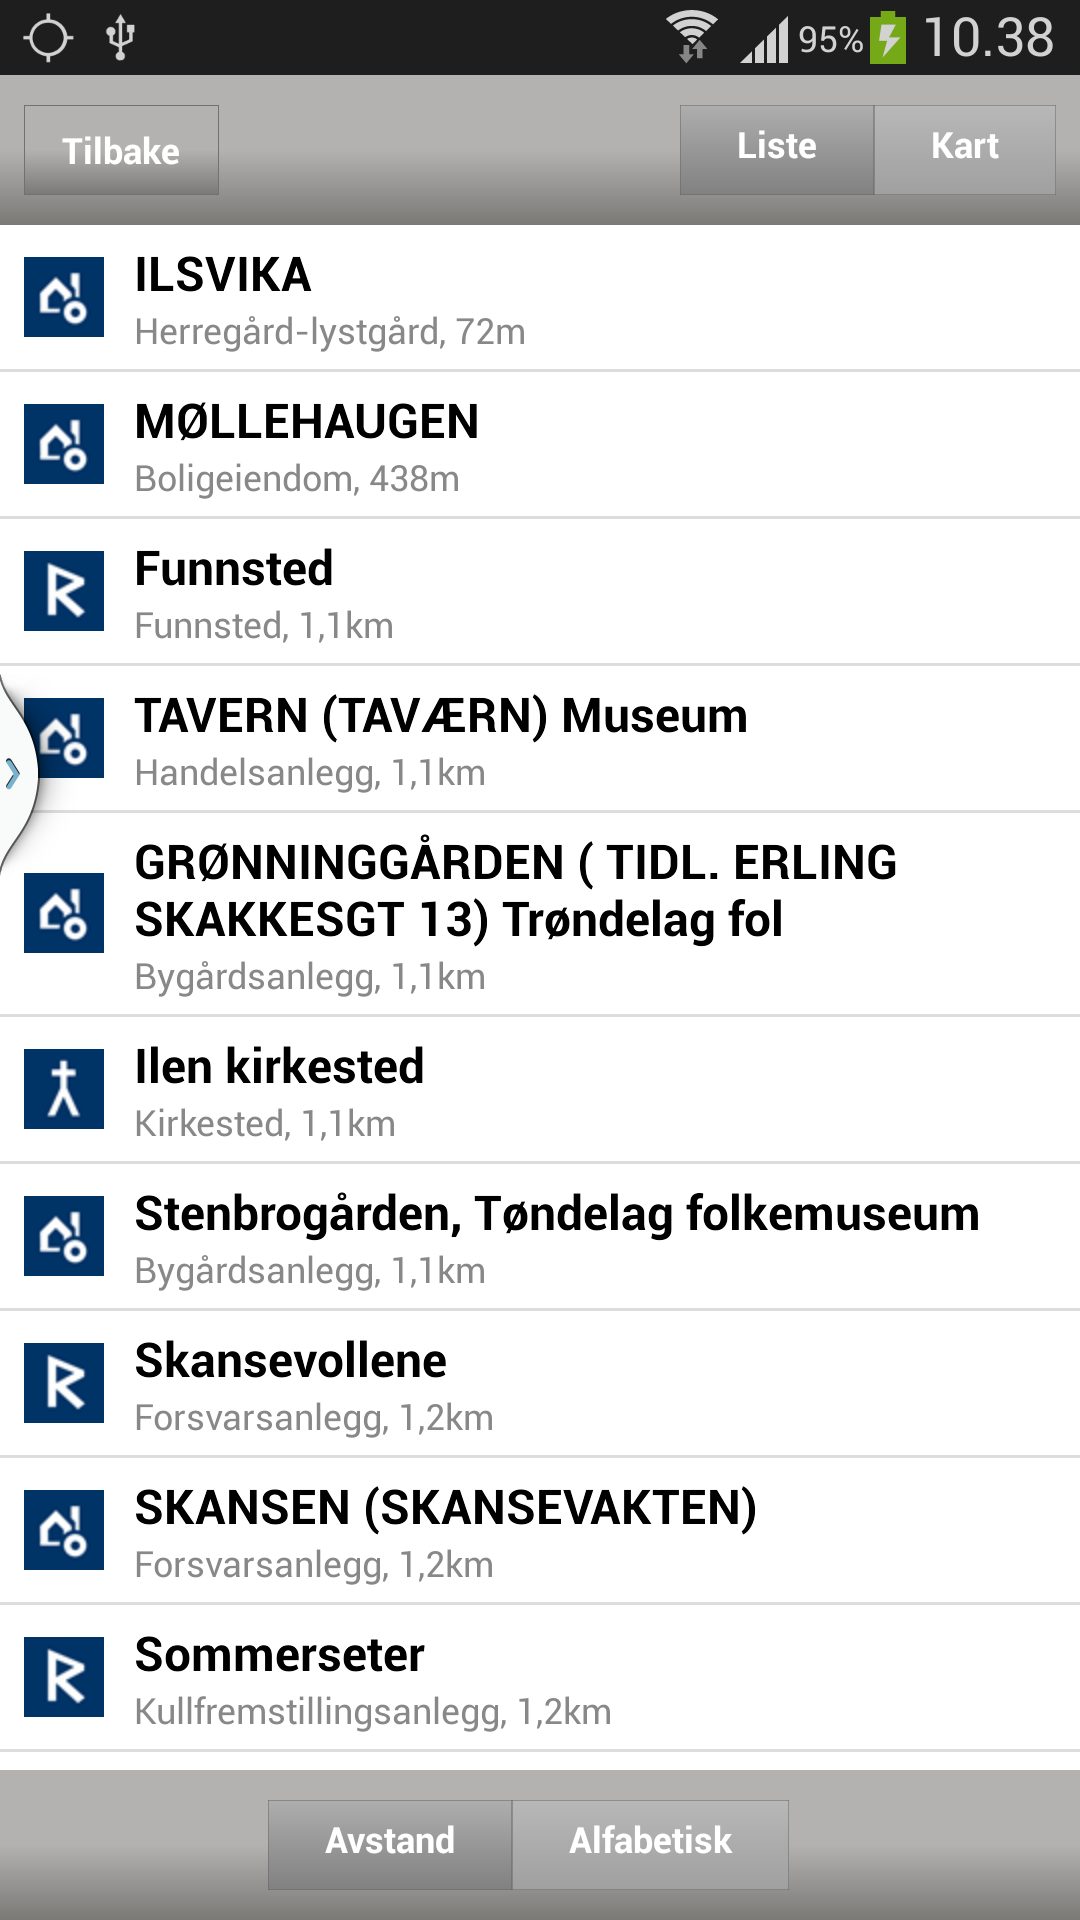
\includegraphics[width=0.4\textwidth]{Figures/Prestudy/kulturSokList.png}
      \caption{Kulturminnesøk, list function}
      \label{fig:pre_kulturMinneAppList}
\end{figure}

\begin{figure}[H]
      \centering
      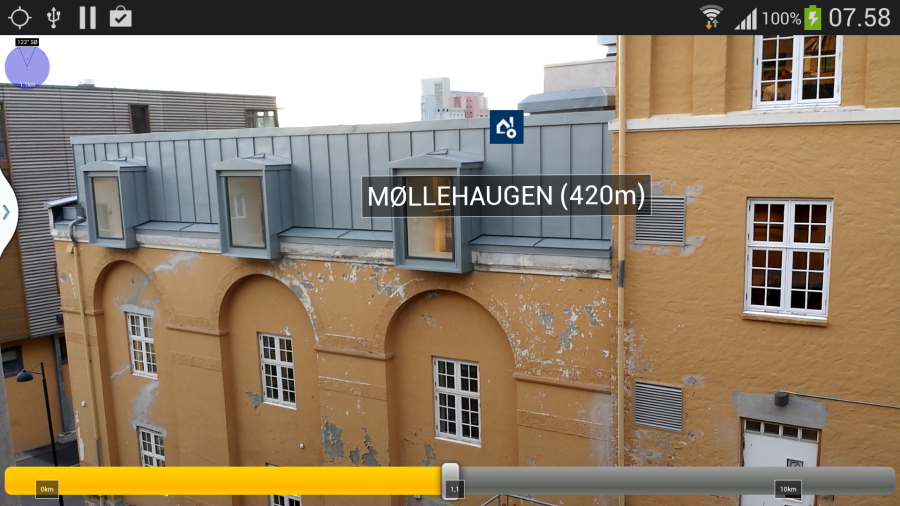
\includegraphics[width=0.8\textwidth]{Figures/Prestudy/kulturSokAR1.png}
      \caption{Kulturminnesøk, augmented reality function}
      \label{fig:pre_kulturMinneAppAug}
\end{figure}

\subsection{Kulturarv app}
Kulturarv, or Cultural Heritage, is a Danish cultural heritage mobile application. It is very similar to the Kultursøk mobile application, it has both a map function, Figure~\ref{fig:pre_kulturArvAppMap}, and a augmented reality function, Figure~\ref{fig:pre_kulturArvAppMap},  to show the user where to find protected and preservation-worthy buildings. It uses the Danish ``Fredede og Bevaringsværdige Bygninger'', or  ``Protected and Preservation-worthy Buildings'', (FBB) web service, which appears to be quite similar to the Askeladden database. It sounds like the danish Kulturarv and Kultursøk is pretty much the same thing, but Kulturarv has one more important functions, which makes it much better; Kulturarv blends the media from FBB and other geolocation data sources like Instagram, Flickr, Wikipedia and Twitter. Unfortunately, we are not able to test the application because it seems to only work if you are physically in Denmark, but we have the impression of how it works through Kulturarv's homepage \cite{Kulturarv}. It is also worth  mentioning that the application is an open-source project released under the GNU GPL v3 license.

\begin{figure}[H]
      \centering
      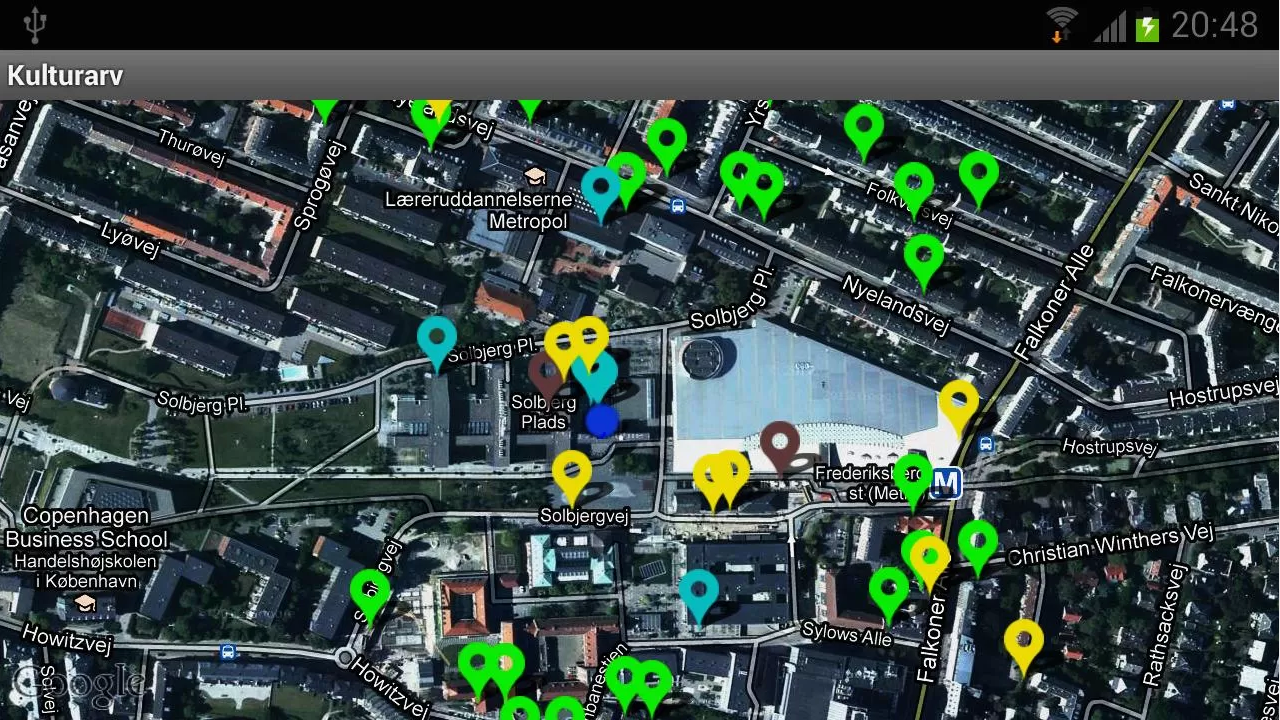
\includegraphics[width=0.8\textwidth]{Figures/Prestudy/kulturArvMap.png}
      \caption{Kulturarv, map function}
      \label{fig:pre_kulturArvAppMap}
\end{figure}

\begin{figure}[H]
      \centering
      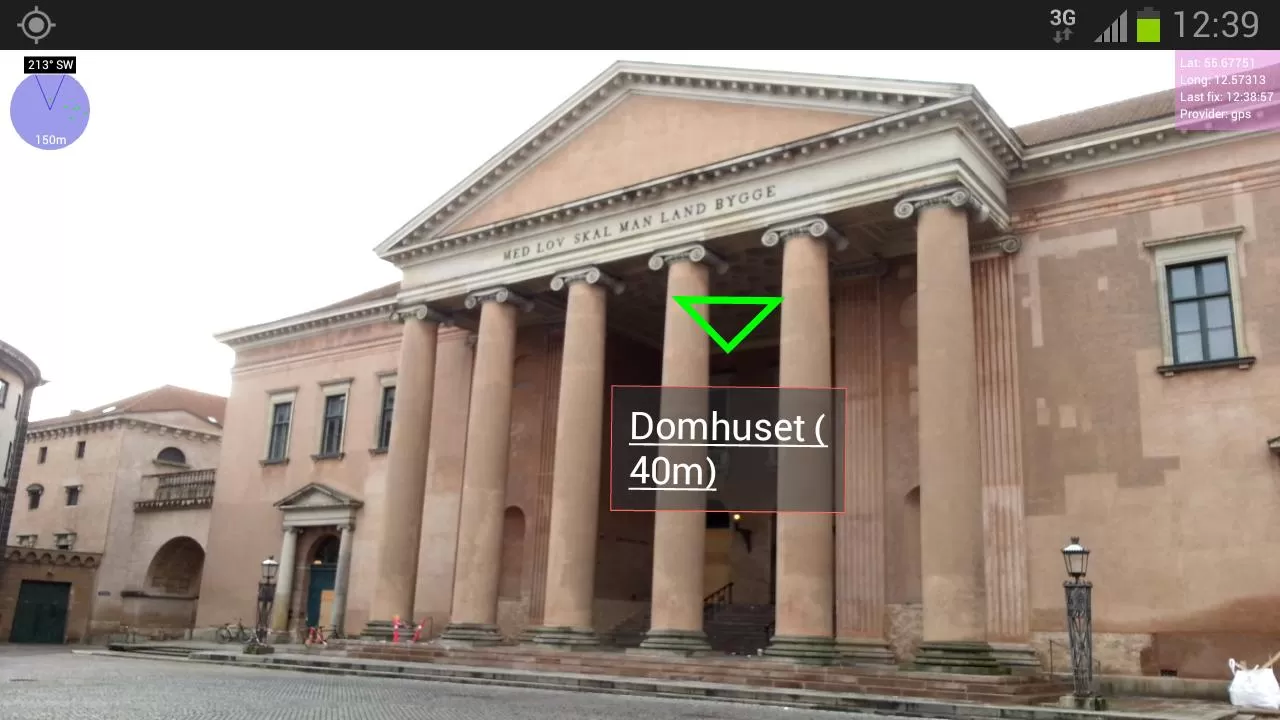
\includegraphics[width=0.8\textwidth]{Figures/Prestudy/kulturArvAR1.png}
      \caption{Kulturarv, augmented reality function}
      \label{fig:pre_kulturArvAppAug}
\end{figure}

\subsection{1001 Stories of Denmark}
Again we are looking at a Danish application that has many similarities with a Norwegian application, namely Digitalt Fortalt. It is called ``1001 Stories of Denmark'', and it lets the user read stories about 1001 places in Denmark, including ancient monuments, architectural buildings and sceneries. You can browse sights with either a map or a list, Figure~\ref{fig:pre_1001StoriesDenmarkAppList} and~\ref{fig:pre_1001StoriesDenmarkAppMap}. When you choose a sight, you can read about the sight in general, read stories about it or look at pictures, Figure~\ref{fig:pre_1001StoriesDenmarkAppStory}. Another function is that you can get predefined routes or make your own routes, that includes the sights you want to see. For example, you can find a route that is about the famous architect and designer Arne Jacobsen (1902 - 1971), that includes visits to buildings that was designed by Arne Jacobsen. In the same way as the previous application, we can not test it because you need to physically be in Denmark.

\begin{figure}[H]
      \centering
      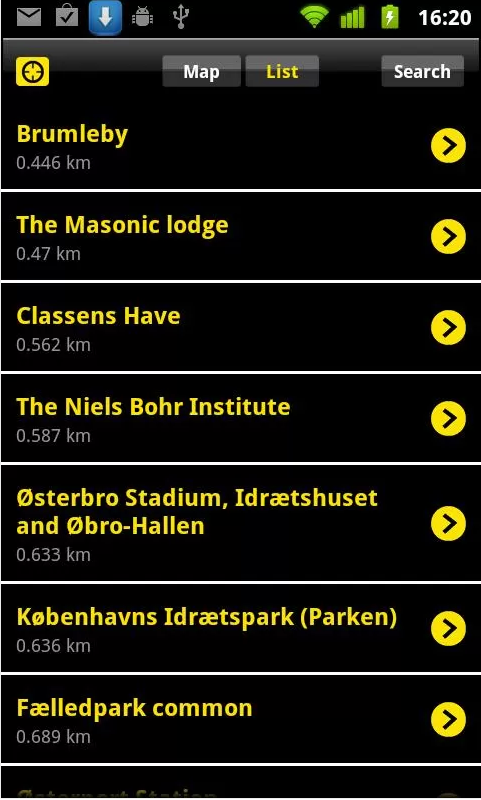
\includegraphics[width=0.3\textwidth]{Figures/Prestudy/1001storiesList.png}
      \caption{1001 Stories of Denmark, list function}
      \label{fig:pre_1001StoriesDenmarkAppList}
\end{figure}

\begin{figure}[H]
      \centering
      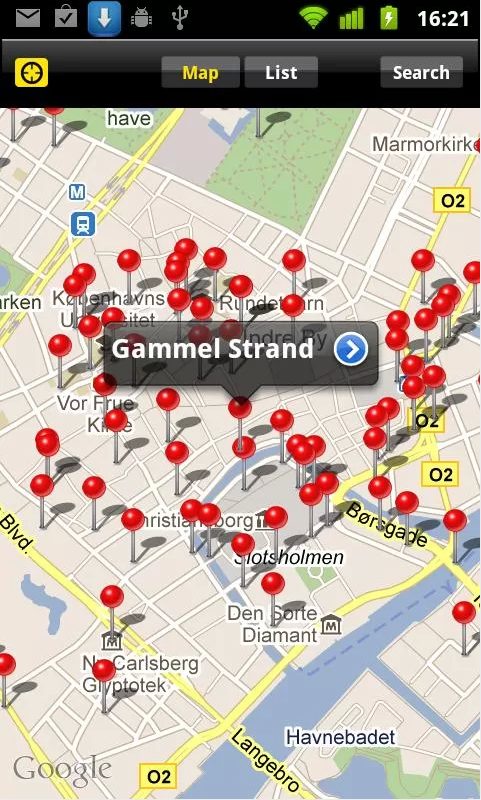
\includegraphics[width=0.4\textwidth]{Figures/Prestudy/1001storiesMap.png}
      \caption{1001 Stories of Denmark, map function}
      \label{fig:pre_1001StoriesDenmarkAppMap}
\end{figure}

\begin{figure}[H]
      \centering
      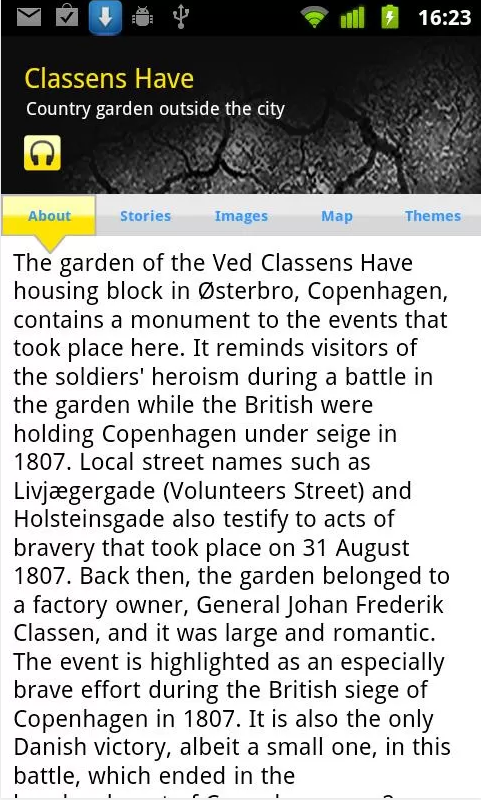
\includegraphics[width=0.4\textwidth]{Figures/Prestudy/1001storiesStory.png}
      \caption{1001 Stories of Denmark, a sight}
      \label{fig:pre_1001StoriesDenmarkAppStory}
\end{figure}

This mobile application also has an associated website \cite{1001fort}, with the same functions as in the mobile application. In addition there is a timeline function, where all the stories with a timestamp appears, Figure~\ref{fig:pre_1001StoriesDenmarkTimeLine}. The website also invites users to create their own profile, that allows them to add and recommend places, add stories, comment on existing stories and to  upload images and videos.

\begin{figure}[H]
      \centering
      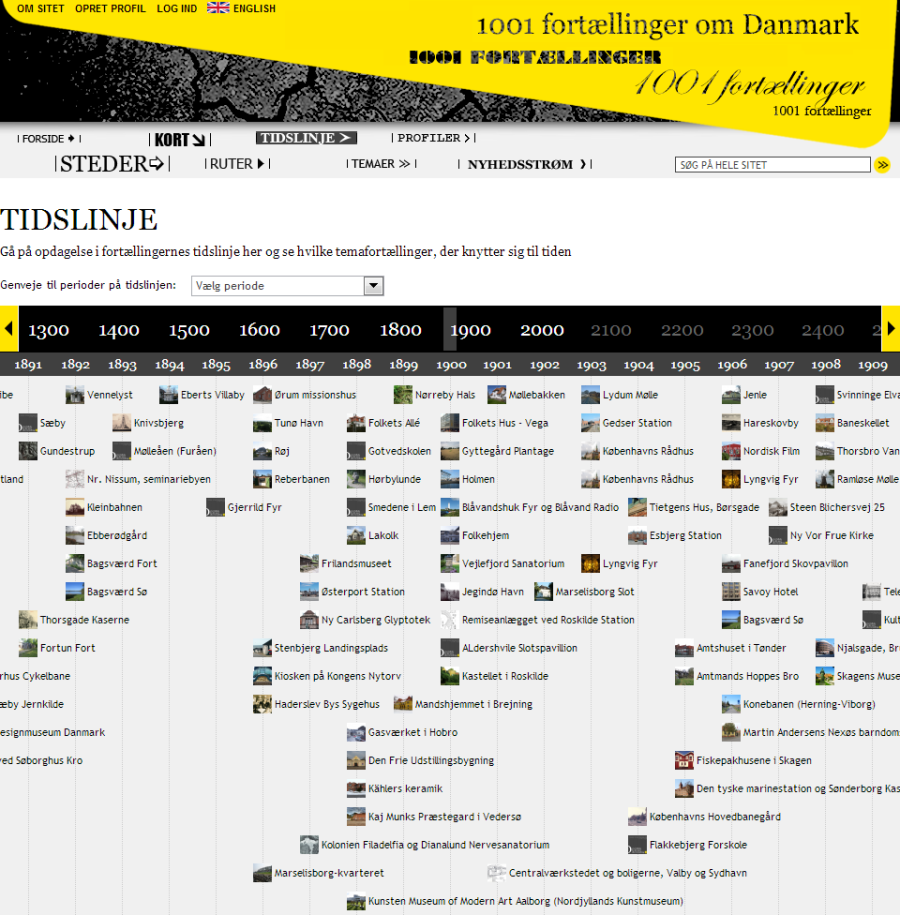
\includegraphics[width=0.8\textwidth]{Figures/Prestudy/1001storiesWebsiteTimeline.png}
      \caption{1001 Stories of Denmark,timeline function}
      \label{fig:pre_1001StoriesDenmarkTimeLine}
\end{figure}

\subsection{Conclusion}
All the applications we have looked at are great pieces of technology. It educates today's generation and helps them discover and learn about our cultural heritage. They are all content-rich applications, and they offers the public to contribute. One thing we have noticed is that nearly every sight, story, place or piece of history are pretty thoroughly made. Perhaps we should focus on a more low-threshold application, so that everyone, even the very young, can participate.
We see that every applications has their own advantages, and we hope that we can purify some of these and perhaps even come up with some new revolutionary features.


\section{Life cycle model}
There are different ways of approaching a project. Two of the more commonly used methods are Waterfall and SCRUM.

\subsection{Waterfall}
The Waterfall model \cite[p. 30-32]{Sommerville10} is derived from general system engineering processes.The work done in a Waterfall model is partitioned in activities. The activities are done sequentially, only when the prior is done, can the consecutive start.

\begin{figure}[H]
      \centering
      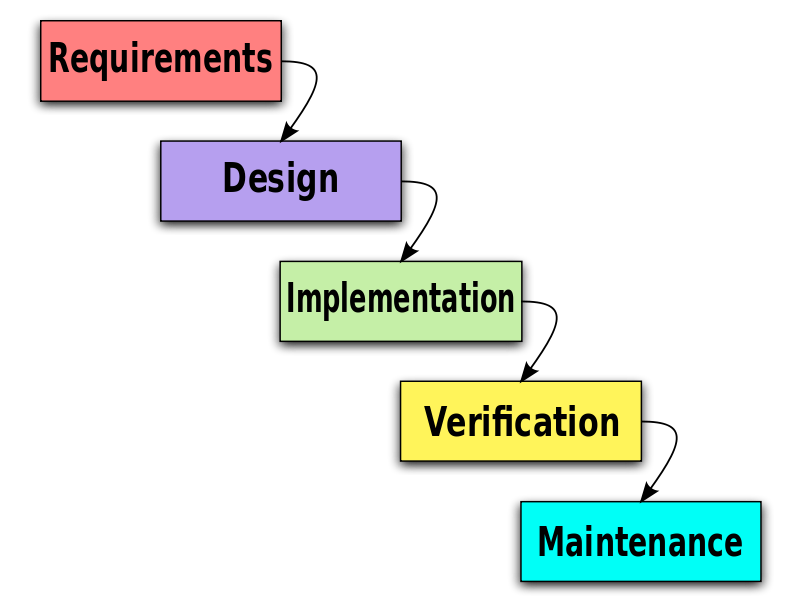
\includegraphics[width=0.8\textwidth]{Figures/Prestudy/Waterfall.png}
      \caption{The Waterfall process \cite{wikipedia:waterfall} without backward duty feedback}
      \label{fig:pre_waterfall}
\end{figure}

Every phase produces one or several documents to be passed on to the next phase. These documents need approval before a phase is considered completed, and the next might start.

Waterfall makes good sense in larger manufacturing environments where certification of every part of the system is required in order to be allowed to manufacture and sell the product. For example the aircraft industry needs detailed plans of the whole aircraft to be certified before manufacturing, and faults could produce devastating effects.

In the original publication about Waterfall for software systems, the author points out some limitations of the model and suggests some project owner involvement.

\begin{quotation}\noindent
For some reason what a software design is going to do is subject to wide interpretation even after previous agreement. It is important to involve the customer in a formal way so that he has committed himself at earlier points before final delivery. To give the contractor free rein between requirement definition and operation is inviting trouble. - According to Royce \cite[p. 335]{DBLP:conf/icse/Royce87}
\end{quotation}

\subsection{SCRUM}
In accordance with the statement from Royce above, SCRUM strive to involve the customer throughout the whole development process. This is done by doing only the strictly required planning and specification writing up front, and then working iteratively with the project together with the customer in sprints. According to \cite[p. 73]{Sommerville10} sprint could last from 2 - 4 weeks and by the end the work is review and result presented for the customer. For each sprint the customer sees the current state of the project and participates in specifying what to do for the next sprint.

\begin{figure}[H]
      \centering
      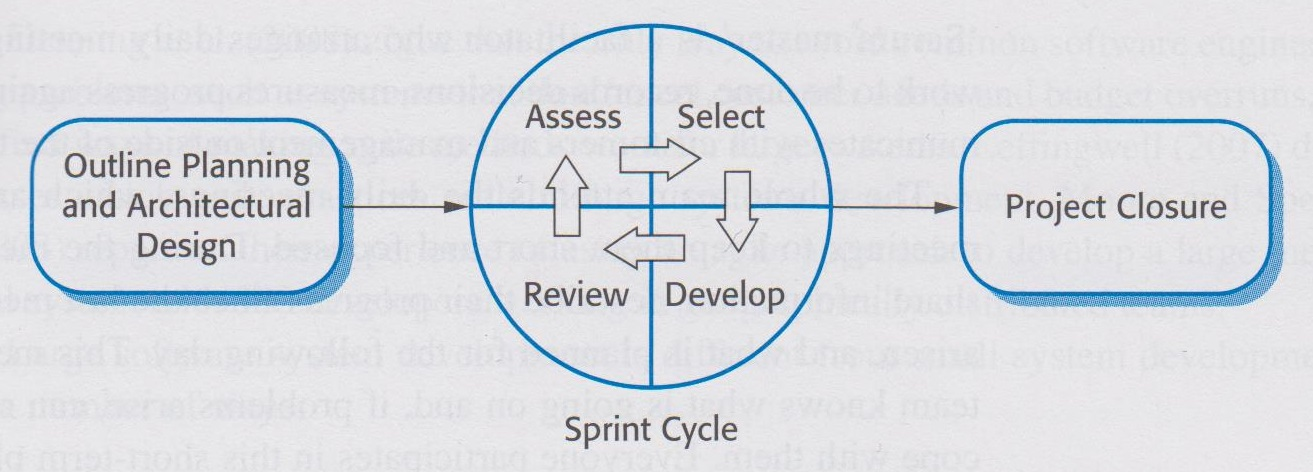
\includegraphics[width=0.8\textwidth]{Figures/Prestudy/SCRUM.jpeg}
      \caption{The SCRUM process}
      \label{fig:pre_scrum}
\end{figure}

This use of continuous customer involvement, helps clarify misunderstandings and correct errors on both the customer's and contractor's side during the process. The fact that this might be caught earlier, means that the project is more likely to deliver on time and on budget.

The customer involvement is primarily within prioritizing and adding items to the backlog which is used as the basis for each sprint. The customer is also involved in clarifying items as they are moved from the backlog to the sprint log.


\subsection{Chosen work methodology}
Given the uncertainties surrounding the concrete goal and plan behind the project, it is beneficial to choose SCRUM to retain a close connection with the customer. This will help resolve any misunderstandings or disagreements about project scope and focus areas.

The customer has experience with SCRUM and suggested the methodology to be used. This will also make it easier to produce a good end project, knowing that we are allowed to refine our documents, requirements and such during the lifetime of the project.

\chapter{Requirements} \label{chap:req}

This chapter is a System Requirements Specification document in the terms of practice recommended by IEEE 830 \cite{ieee830}, developed by the group based upon the customers requests.

\section{Introduction}

\subsection{Purpose}
The purpose of this \gls{srs} document is to provide documentation of requirements for the VirtualWall software system. It is therefore trying to collect and analyze the requirements. The requirements formalization as presented is a result of a joint effort of the customer and the development team. It serves as a description of what customer is expecting the system to be like, it presents the systems features and functionalities.

The intended audience of this document shall be:

\begin{enumerate}
  \item development team (students)
  \item customer (SINTEF ICT, eTrøndelag/Sør-Trøndelag fylkeskommune)
  \item course responsibles (advisor, etc.)
\end{enumerate}

Each part of the audience holds different stakes in the project, but all are interested in information contained within the \gls{srs}.

\subsection{Scope}
This secton declares the scope of this requirements document and the desired output of the project. It shall state what parts of the system shall be analyzed, designed and implemented and to what extent.

This \gls{srs} document deals with the project Virtual walls - walls that tell us stories. This project shall result in developing a tool for working with so called virtual walls, creating and sharing stories on them.

As presented by customer, the VirtualWall software system is going to be a complex system consisting of a number of subsystems including several content databases, a server backend and mobile application frontend.

In the scope of this year's run of Customer Driven Project course, a prototype of a mobile application frontend and a basic server backend shall be developed.

\subsection{Definitions, acronyms and abbreviations}
All definitions, acronyms and abbreviations are listed in the glossary instead.

\subsection{Overview}
The rest of this \gls{srs} document describes the proposed product by means of its desired functionality, characteristics, constraints and perspectives. This general description can be found in section~\ref{sec:req_overall_description}. A description of the actual requirements is to be found in section~\ref{sec:req_specific_requirements}.

\section{Overall description}\label{sec:req_overall_description}
\subsection{Product perspective}
As stated above, the whole system will consist of several subsystems such as the frontend, server backend, own database and external content databases. This implies the use of client-server model.

The components developed in this phase of the project are:

\begin{enumerate}
  \item mobile/web application (frontend)
  \item server (backend)
\end{enumerate}

Customer requires that the tool shall be available for PCs, tablets and mobile phones (smartphones). The prototype shall be optimized for a tablet preferably.

The following diagram shows the whole system and how the separate parts work together.

\begin{figure}[H]
      \centering
      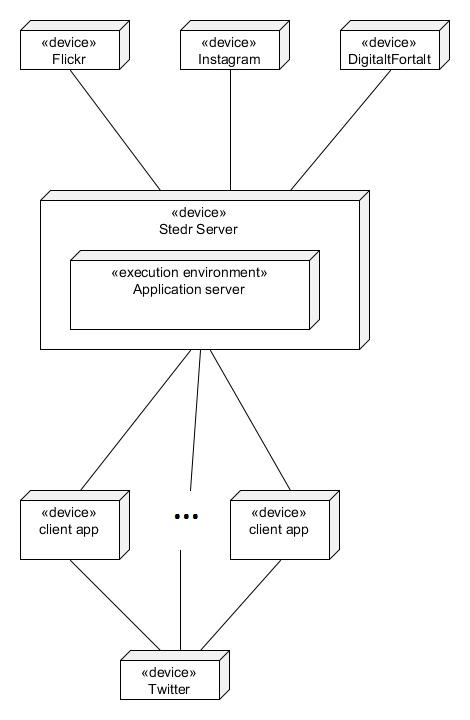
\includegraphics[width=0.8\textwidth]{Figures/Architecture/deploymentView.jpg}
      \caption{Overview of interaction}
      \label{fig:req_overview}
\end{figure}

In the initial phase, the server will not be directly connected to any external content databases machine, the content from them would be presented as simple hyperlinks leading to the third party website (such as kulturminnesok.no, digitaltfortalt.no).

\subsection{User Interfaces}
Since the frontend of the whole system shall be developed in this project, the description of user interface shall be considerably stressed.

We can characterize the nature of the system as crowdsourced (or edge-dominant, in general), as the content shall be generated and modified by users to some extent. Due to this, there is not going to be any backend for data entry, the only point where the system is exposed to human beings is the mobile application frontend.

Our key quality attribute, usability, relates tightly to user interfaces. For this reason, all usability-related requirements on user interface are listed in section \ref{sec:req_software_system_attributes} as quality attribute requirements.

\subsubsection{Mobile application (frontend)}\label{sec:req_webapplication_frontend}
As user requests that the initial prototype application shall be developed for use on tablets. Typical usage of the system suggests that it will be used in field, which implies using the application on smartphones and tablets.

Both smartphones and tablet have some inherent characteristics that have to be respected when designing the user interface and the means of interacting with it.

The screen sizes of current smartphones vary a lot, with the most phones with screen size from 3.5 inches (9 cm) up to 5.5 inches (14 cm). Screen sizes of tablets vary between values from 9 inches (22 cm) to 11.5 inches (29 cm). In addition, these devices can be used in either landscape or portrait mode.

Such a diversity in screen sizes makes designing the user interface very challenging. On one hand, we want to maximize the screen usage even on large-screen devices, on the other hand, we must make the application usable even on devices with screen area up to 9 times smaller.

Another characteristic property of those devices is that their interaction mechanisms are somewhat limited.

\begin{enumerate}
  \item These devices are generally missing a mouse, and thus a mouse cursor. Direct pointing is done by using finger upon touchscreen. This is however less precise, so the user interface must be accustomed to that.
  \item Devices usually miss a hardware keyboard. This is surrogated by having a software keyboard on-screen. This however takes up some of the valuable screen real estate. This kind of keyboard is additionally not as usable as a real hardware one, so the user is not tempted to use it as much., therefore use of any hotkeys is out of question.
\end{enumerate}

\subsection{Software interfaces}
We imply that the server and the client interoperate and are developed to work with one another. The required interfaces and communication schema is to be determined later on in section \ref{sec:arch_communicationinterfaces}.

\subsection{Communication interfaces}
This section describes what we shall take into account when designing interfaces for communication between subsystems of our system. If there are any special characteristics of the environment that affect those interfaces, they should be stated here.

Another inherent characteristic of mobile devices (smartphones, tablets, etc.) is the unreliability and speed of network connection. Since this application is a part of a client-server system, the communication link between those is critical.

The main issues with mobile data networks are frequent interruption, big latency and small bitrate. Sometimes the connection can as well be unavailable at all. This results in the data connection being slow and unreliable which has a great significance on the performance of the application and its usability. As developers of the mobile application, we need to take this into consideration.

There are several techniques how to deal with mentioned issues or at least mitigate their impact.

\subsubsection{Unavailability of connection}\label{sec:req_unavailability_of_connection}
To deal with frequent interruption and unavailability of connection, an off-line mode of the application could be implemented in the future, which would enable the user to work without a network connection (in a limited way).

This was described by the customer as to be a low priority requirement, not to be implemented in this phase.

\subsubsection{Small throughput}
To deal with small throughput of the network, the updates of the content in the client application could be implemented using delta updating. This would mean only new and changed data are sent from the server, data that did not change are used from the local storage.

This issue is not to be addressed in this phase of the project and may be implemented later on.

\subsection{Product functions}

\subsubsection{Frontend}
The key functionality expected in the frontend is management of virtual walls (creating, editing), stories on them (creating, editing) and social interaction (commenting, sharing).

\subsubsection{Backend}
The key functionality of the server is to support the features of the client by storing the data in the database and retrieving it back. As said above, the content is stored in the system database. The server shall expose an API for accessing the items from database (walls, stories) for access from the frontend.

\subsection{User characteristics} \label{sec:req_user_characteristics}
As this app shall be accessible to open public, we can neither anticipate users' educational level, nor experience, nor technical expertise. We can however assume basic computer literacy.

Documentation from customer features a scenario how this application would be used in class in elementary school. We may anticipate that some of the users can be as young as 10 years for example.

See chapter \ref{sec:req_usability} for requirements on usability.

\subsection{Constraints}

This section lists the design constraints prescribed by the customer, such as use of specific languages, toolkits or frameworks.

\subsubsection{HTML5 use}
Since use on many different devices and platforms is expected and necessary, customer requested that the frontend would be a mobile application. As the system is crowdsourced and heavily relies on users, it it necessary that it interacts very well with the users and is visually appealing. Also, for reasons stated in \ref{sec:req_unavailability_of_connection}, local storage is necessary to enable off-line mode (in the future). This implies the use of cutting-edge technologies for the development.

For this reason, customer suggests that the application will be developed in HTML5.

\section{Specific requirements}\label{sec:req_specific_requirements}

\subsection{External interfaces}
As the application developed is going to be a client/server where the client is a mobile/web application, we will use \gls{http} protocol for data exchange. Data transferred over \gls{http} in our case will be in \gls{json} format.

\subsubsection{Virtual Wall Client/Server interface}
VirtualWall client is a mobile that runs in a container similar to a web browser. Once the application is installed in the phone and open, data transfers with the web server can be done using \gls{ajax} to retrieve the data in \gls{json} format from the server.

Format of the messages is presented in sections \ref{placesjson}, \ref{storiesjson} and \ref{imagesjson}.

\subsubsection{Social networks}\label{sec:req_social_networks}
Walls and stories shall be easily shared using social networks like Facebook or Twitter. Custom button for sharing/liking shall be available for each story or wall that user wants to like or share.

Sharing in this case means posting a link on user's social network profile.

\subsection{Functions}\label{sec:functionalreq}
The functional requirements are organized according to object categories.

\subsubsection{Places}

\begin{table}[H]
\centering
\begin{tabular}{ l  p{11cm} l }
    ID       & Description                                                                                              & Test level            \\ \hline
    F2.2     & System shall let users filter and view places                                                            & All                   \\ \hline
    F2.2.2   & System shall let users to filter places by tags                                                          & System, Unit, UAT     \\ \hline
    F2.2.3   & System shall let users to filter places by metadata (location)                                           & System, Unit, UAT     \\ \hline
    F2.2.4   & System shall let users to filter places by story authors                                                 & System, Unit, UAT     \\ \hline
    F2.4     & System shall let users like and share places over social networks (facebook, twitter). 
               See \ref{sec:req_social_networks} for details                                                            & System, Unit, UAT     \\ 
\end{tabular}
\caption{Walls}
\label{tab:req_walls}
\end{table}

\subsubsection{Stories}

\begin{table}[H]
\centering
\begin{tabular}{ l  p{11cm} l }
    ID       & Description                                                                                              & Test level            \\ \hline
    F3.2     & System shall let users filter and view stories from a particular places                                  & All                   \\ \hline
    F3.2.2   & System shall let users to filter stories by tags on a particular places                                  & System, Unit, UAT     \\ \hline
    F3.2.4   & System shall let users to filter stories by metadata (author, media duration) on a particular places     & System, Unit, UAT     \\ \hline
    F3.3     & System shall let users comment on stories                                                                & System, Unit, UAT     \\ \hline
    F3.4     & System shall let users like and share stories over social networks (facebook, twitter). 
               See \ref{sec:req_social_networks} for details                                                            & System, Unit, UAT     \\
    \end{tabular}
\caption{Stories}
\label{tab:req_stories}
\end{table}

\subsubsection{Images}

\begin{table}[H]
\centering
\begin{tabular}{ l  p{11cm} l }
    ID       & Description                                                                                              & Test level            \\ \hline
    F4.1     & System shall show images tagged with the tag of the particular place.                                    & All                   \\
    \end{tabular}
\caption{Stories}
\label{tab:req_images}
\end{table}

\subsection{Quality attributes}\label{sec:req_software_system_attributes}
In this section, we describe several quality attributes this system shall have.

\subsubsection{Maintainability}
Customer stated that the system shall be well documented and easily extensible and modifiable. These concerns are related to the quality attribute of maintainability.

Customer requests that the project documentation shall include description of all interfaces, architectural description and sequence diagrams to illustrate how does the system work.

\subsubsection{Portability}
As customer requested, the front end application shall be developed in order to be working on various devices, ranging from small smartphones to desktop stations.

Quality attribute scenario to evaluate the system shall be determined in section \ref{sec:qatestscenarios}.

\subsubsection{Usability}\label{sec:req_usability}
From the description of typical usage (mentioned in \ref{sec:req_user_characteristics}) and characteristic problems listed in \ref{sec:req_webapplication_frontend}, we came up with several usability scenarios that shall evaluate the usability quality of the software system. As usability is a big concern in this project, usability scenarios and tests shall be included in the report under Test Procedures Specification.  % FIXME SIMON: once usability tests are prepared, put refs to them (link to Test Procedures Specification)

These scenarios shall evaluate, whether the application suits the needs of the audience in the means of usability. These shall be derived from use cases and requirements.

\section{Use cases}

According to \cite{usecases}, use case is a description of actions users are performing with the software system. In our case, the use cases are indifferent from test cases of frontend functional requirements that are specified later on in section \ref{sec:fe-test-cases}. We decided not to duplicate the information within this report.

As there is just few requirements left after all the changes made, we are presenting all of them in just one use case diagram. Their textual description can be found in functional requirements tables above, in section \ref{sec:functionalreq}.

\begin{figure}[H]
      \centering
      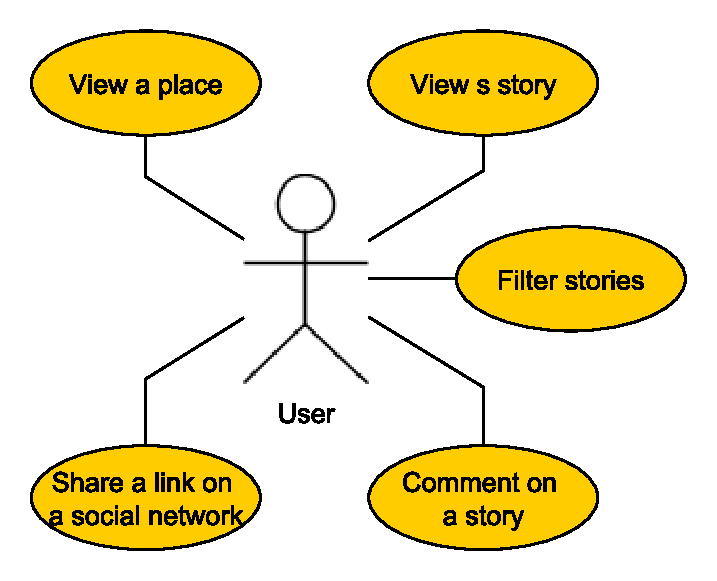
\includegraphics[width=0.5\textwidth]{Figures/Requirements/final.pdf}
      \caption{Use case diagram for Places}
      \label{fig:req_usecase_walls}
\end{figure}

\chapter{Software System Architecture}\label{chap:architecture}
The following architecture is the result of the group working closely with the customers requirements and trying to fulfill them as elegantly and sustainably as possible.

For the client application, creating an architecture satisfying the customers requirements, was not too hard. It was  mainly based upon recognized industry patterns.

Designing the server, which uses multiple external systems, without introducing multiple points of failure, proved to be more difficult. In the end, the server was designed with recognized industry patterns at least allowing it to fail gracefully.

\section{Architectural drivers} \label{sec:architecture_drivers}
In the following the document, the items listed bellow have been used as the main drivers for the architecture.

\subsection{Maintainability} 
A maintainable code base makes for a developable code base. Achieving a maintainable base will make development easier in the short run and maintenance less expensive in the long run. It will also be easier for other teams to continue the development upon the same code base.\\
Quality requirement: Modifiability

\subsection{Portability}
The customer requested that the system should be usable on different smartphone platforms and also on a normal computer. As such portability is key in order to lighten the workload required to achieve this goal.\\
Quality requirement: Modifiability

\subsection{Division between logic and presentation}
Division between logic and presentation makes the system more modular and modifiable.\\
Quality requirement: Usability, Modifiability

\subsection{Short development time}
Given the relatively short duration of this project, the architecture should make for fast development, while not sacrificing quality.

\section{Stakeholders and concerns}

\subsection{Developers}
The architects and developers are concerned about ease and speed of development. As part of this one also has to consider the elegance of the resulting architecture. This is import to make it more understandable for those who are to continue the development or maintain an operational system.

\subsection{Customer}
The customer is interested in seeing a highly usable system that can run on multiple different devices and be easy to build upon, should they decide to use the prototype as starting point for an actual product.

\subsection{End users}
End users are mostly concerned about the ease of use of the system. This includes the stability and performance as well as the normal usability.

\subsection{Course staff}
The course staff is mostly concerned about the quality of the documentation and its readability.

\section{Selection of Architectural views}
``The 4+1 View Model of Software Architecture'' \cite{Kruchten:1995:VMA:624610.625529} outlines several ways of presenting different aspects of the architecture, useful to different persons. The article uses a variant of Booch syntax to visualize the views, but in this document we will use standard UML diagrams.

This description will focus on the first three views, logical, process and development view.

\subsection{Logical view}\label{subsec:logicalViewDescription}
Purpose: The logical view will give us an understanding of how to layout our code in a meaningful way. It will show how classes and modules relates to each other, and as such help us identify common relations and tasks and then generalize them.\\
Stakeholders: Developers, course staff\\
Form of description: Class diagram

\subsection{Process view}\label{subsec:processViewDescription}
Purpose: The process view serves to show how the modules and classes communicates with each other, and explain the system processes.\\
Stakeholders: Developers, Customer, End users, Course staff\\
Form of description: Sequence diagrams

\subsection{Development view}\label{subsec:developmentViewDescription}
Purpose: The main matter of concern for the development view is the development process. It serves to show which parts of the system depends upon others. \\
Stakeholders: Developers\\
Form of description: Architecture Layer Diagram

\subsection{Deployment view}\label{subsec:deploymentViewDescription}
Purpose: The deployment view serves to get a overview of how the system interrelate.
Stakeholders: Developers
Form of description: Deployment diagram

\section{Architectural Tactics}

\subsection{Modifiability}

\subsubsection{Increase cohesion}
By making every part of the system do only one thing, but do it well, it will be easier to change parts of the system or reuse it in other parts.

\subsubsection{Decrease coupling}
By reducing the coupling the change or modification of parts of the systems will have less impact on the rest of the system. Thus making modifications easier.

\subsubsection{Information hiding}
Information hiding allows to provide a stable internal API. This will reduce development time, increase testability and also provide better modifiability.

\subsection{Usability}

\subsubsection{User initiative}
By allowing the user to abort operations, undo or redo the user will feel more comfortable and secure while using the application.

\subsection{Testability}

\subsubsection{Limit complexity}
By doing what can be done simple, in a simple way, the system will be less complicated to test and more likely than not have less bugs.

\subsubsection{Local state}
By keeping the state local, the complexity of state machines with multiple participants are avoided. Make central access point stateless, and keep track of the state on the local devices.

\section{Architecture and design patterns}

The overall architecture for the whole system is client-server, where the handheld device or the web browser requests information from the server, which in turn returns it. The advantage of using client-server is that multiple devices might access the same information without needing to download an entire library every time someone updates some information. Using client-server instead of peer-to-peer simplifies keeping the integrity of the information and securing the users data.

\subsection{Client}
On the client, Model View Controller will be used in order to separate concerns and keep the code as clean as possible. By dividing user interface, data and logic in different blocks, we increase modifiability and maintainability as well as increasing the speed of development as subdividing tasks will be easier.

Appcelerator Titanium will be used as an adapter to different platforms, this be Android, iOS or a normal browser.

\subsection{Server}
The server will be a stateless \gls{rest} services built on Play Framework. This gives a simple client-server approach where the server consists of some simple layers.

The server will be fully stateless which will help on scalability and availability as well as simplifying modifiability. It will also act as an broker, and therefor follow the broker pattern.

\section{Views}

\subsection{Server}

\subsubsection{Logical view}
This view follows the description in section ~\ref{subsec:logicalViewDescription}

The logical view is quite simple due to the fact that Play! Framework is doing most of the heavy lifting. Each logical entity has its own controller/model pair that handles fetching, storing and modifying the relevant information.

\begin{figure}[H]
      \centering
      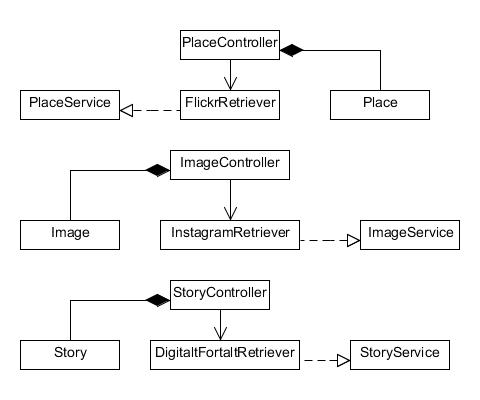
\includegraphics[width=1.0\textwidth]{Figures/Architecture/serverLogical.jpg}
      \caption{Server - Logical view}
      \label{fig:arch_server_logical}
\end{figure}

\subsubsection{Process view}
This view follows the description in section ~\ref{subsec:processViewDescription}

The process in the server is quite simple as it is modeled on the way \gls{http} works, and the way browsers threats \gls{html}. The client sends a request to an URL and the Play! Frameworks main controller delegates the  responsibility of delivering data to the correct controller based on the URL requested. If the content received has connections to other types of content on the server, the client will have to send a new request for that content.

\begin{figure}[H]
      \centering
      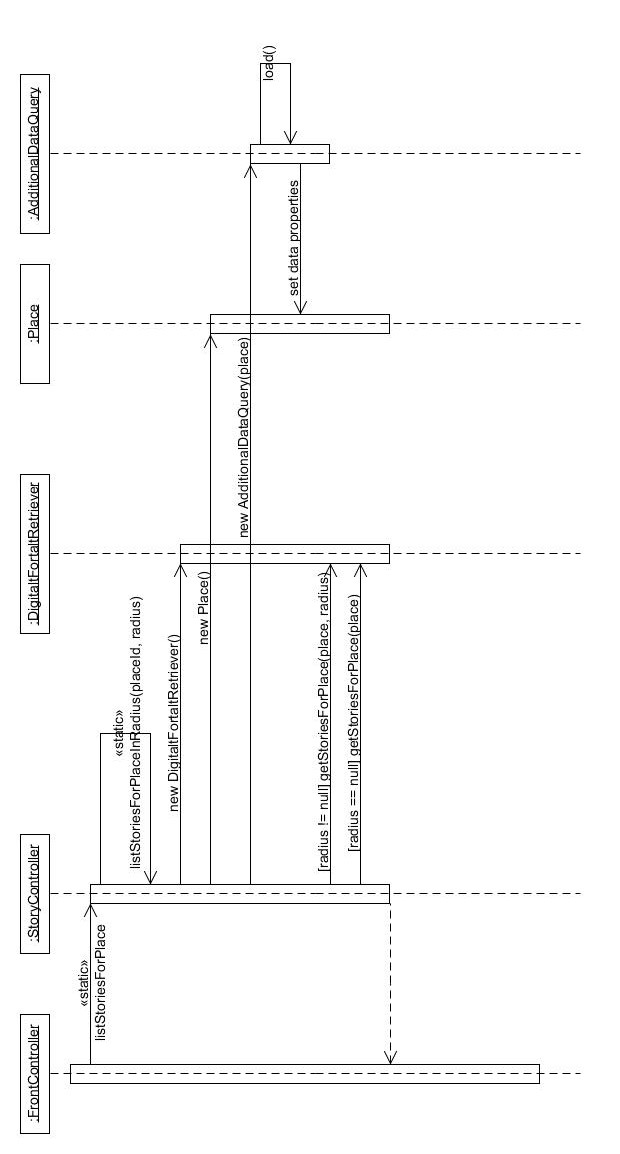
\includegraphics[width=0.8\textwidth]{Figures/Architecture/Sequence/story.jpg}
      \caption{Server - Process view for fetching stories}
      \label{fig:arch_server_process_story}
\end{figure}

\begin{figure}[H]
      \centering
      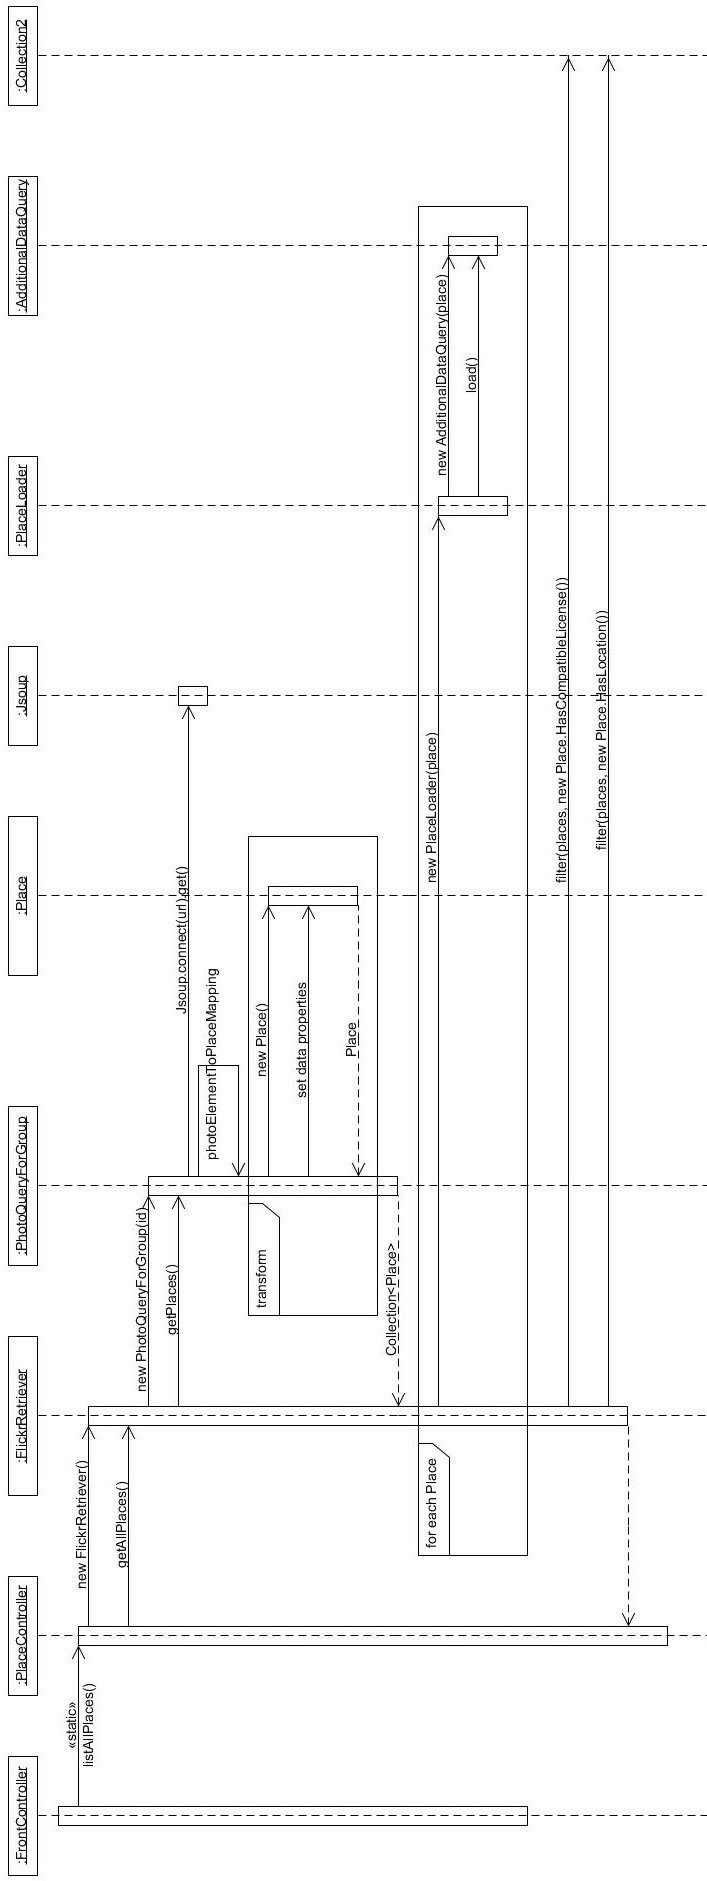
\includegraphics[width=0.6\textwidth]{Figures/Architecture/Sequence/place.jpg}
      \caption{Server - Process view for fetching places}
      \label{fig:arch_server_process_place}
\end{figure}

The retriever for places from Flickr has some additional functionality in order to support local caching to increase the performance of the system.

\begin{figure}[H]
      \centering
      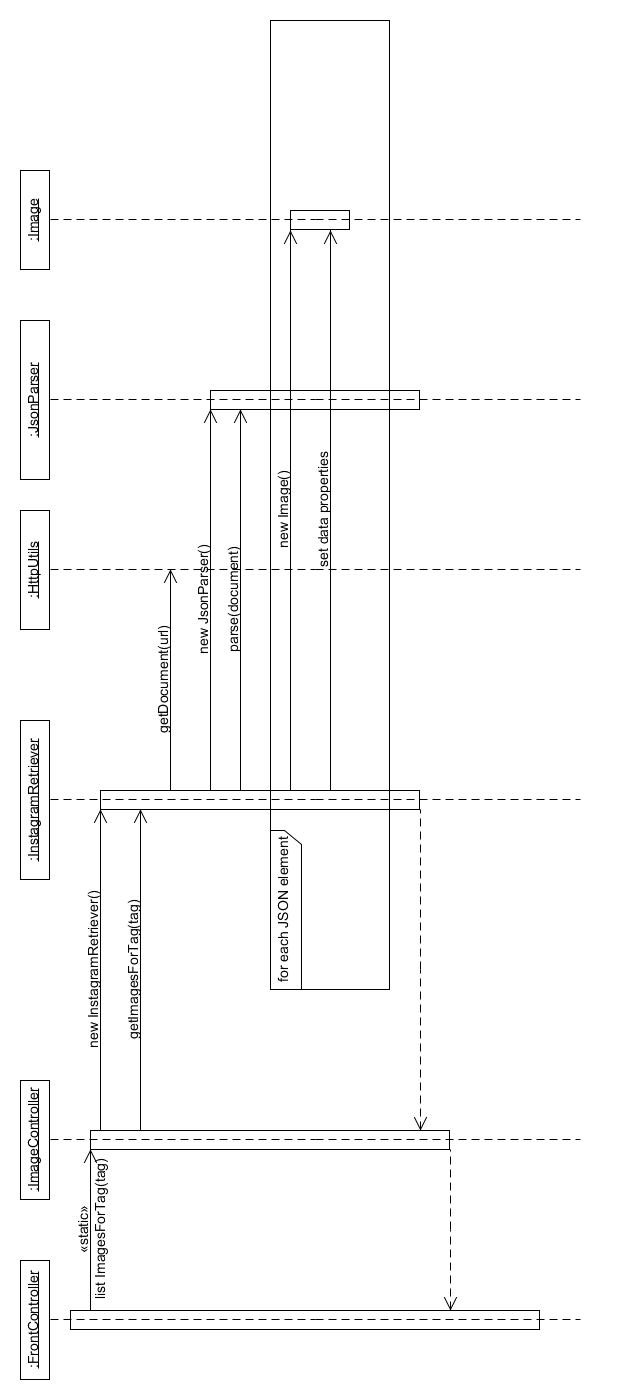
\includegraphics[width=0.6\textwidth]{Figures/Architecture/Sequence/image.jpg}
      \caption{Server - Process view for fetching user images}
      \label{fig:arch_server_process_image}
\end{figure}

\subsubsection{Development view}
This view follows the description in section ~\ref{subsec:developmentViewDescription}

DATA STRUCTURE indicates where and in which format the data is to be stored.

MODELS represents the classes that will be used to work with the database from the rest of the backend code. The models will abstract away the database, so that it can be changed in its entirety if needed without changing any other code.

CONTROLLERS represents the classes that handles the requests and returns data to the client or sends it to the model for storage in the database.

\begin{figure}[H]
      \centering
      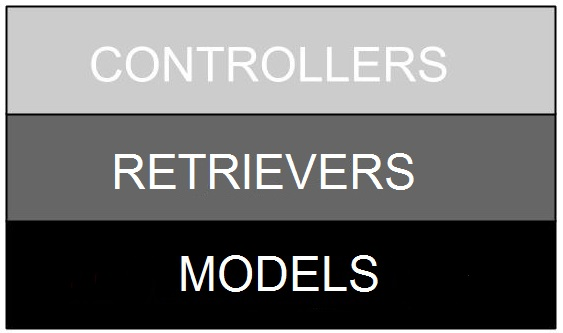
\includegraphics[width=0.8\textwidth]{Figures/Architecture/serverDevelopment.jpg}
      \caption{Server - Development view}
      \label{fig:arch_server_development}
\end{figure}

\subsection{Client}

\subsubsection{Logical view}
This view follows the description in section ~\ref{subsec:logicalViewDescription}

\begin{figure}[H]
      \centering
      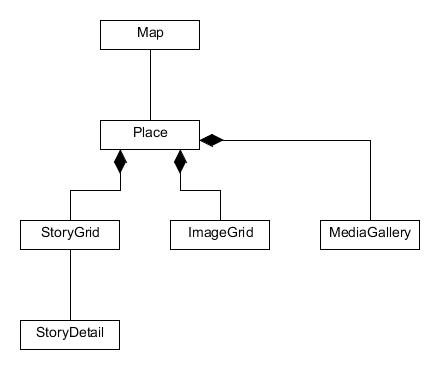
\includegraphics[width=1.0\textwidth]{Figures/Architecture/clientLogicalController.jpg}
      \caption{Client - Logical view of controllers}
      \label{fig:arch_client_logical_controllers}
\end{figure}

\begin{figure}[H]
      \centering
      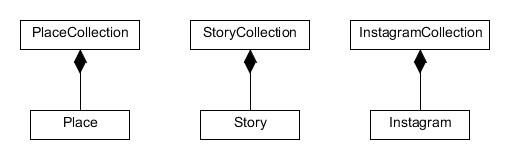
\includegraphics[width=0.5\textwidth]{Figures/Architecture/clientLogicalModels.jpg}
      \caption{Client - Logical view of models}
      \label{fig:arch_client_logical_models}
\end{figure}

\begin{figure}[H]
      \centering
      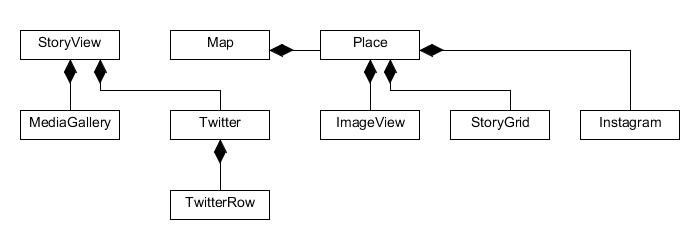
\includegraphics[width=1.0\textwidth]{Figures/Architecture/clientLogicalViews.jpg}
      \caption{Client - Logical view of views}
      \label{fig:arch_client_logical_views}
\end{figure}

\subsubsection{Process view}
This view follows the description in section ~\ref{subsec:processViewDescription}

All the states in the Figures ~\ref{fig:arch_client_process_map}, ~\ref{fig:arch_client_process_stedrWall}, ~\ref{fig:arch_client_process_story} and ~\ref{fig:arch_client_process_storyDetail} have a back event in addition to those added. They were left out in order to simplify the figures.

\begin{figure}[H]
      \centering
      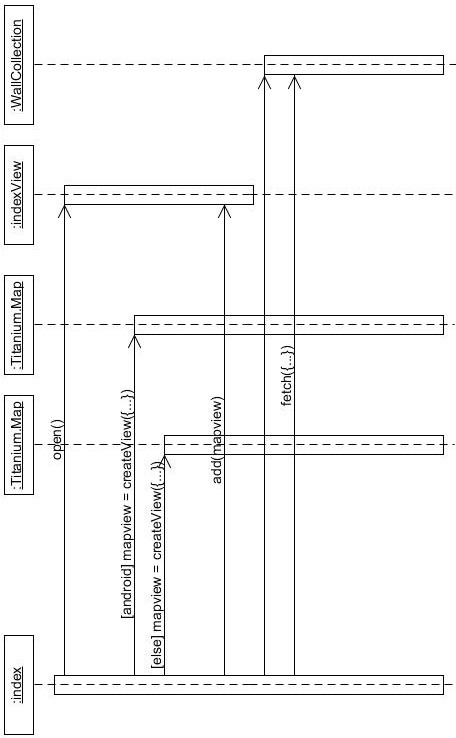
\includegraphics[width=0.8\textwidth]{Figures/Architecture/Sequence/client/map.jpg}
      \caption{Client - Process view of map}
      \label{fig:arch_client_process_map}
\end{figure}

\begin{figure}[H]
      \centering
      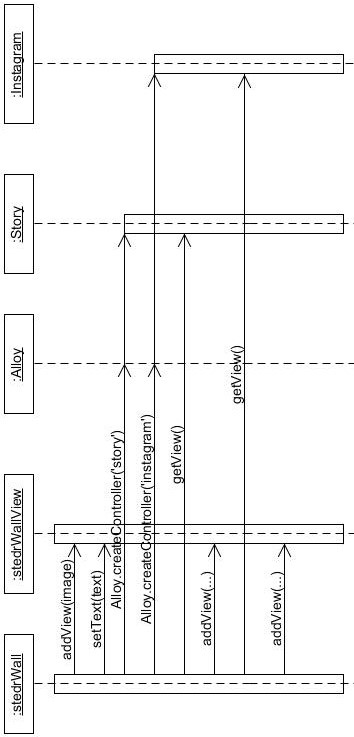
\includegraphics[width=0.8\textwidth]{Figures/Architecture/Sequence/client/stedrWall.jpg}
      \caption{Client - Process view for detail view of place}
      \label{fig:arch_client_process_stedrWall}
\end{figure}

\begin{figure}[H]
      \centering
      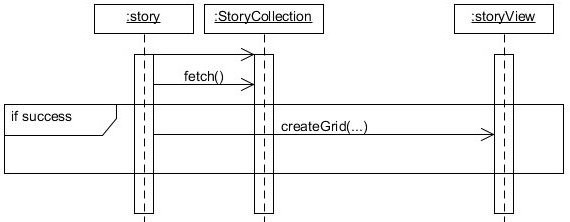
\includegraphics[width=1.0\textwidth]{Figures/Architecture/Sequence/client/story.jpg}
      \caption{Client - Process view for grid view with stories}
      \label{fig:arch_client_process_story}
\end{figure}

\begin{figure}[H]
      \centering
      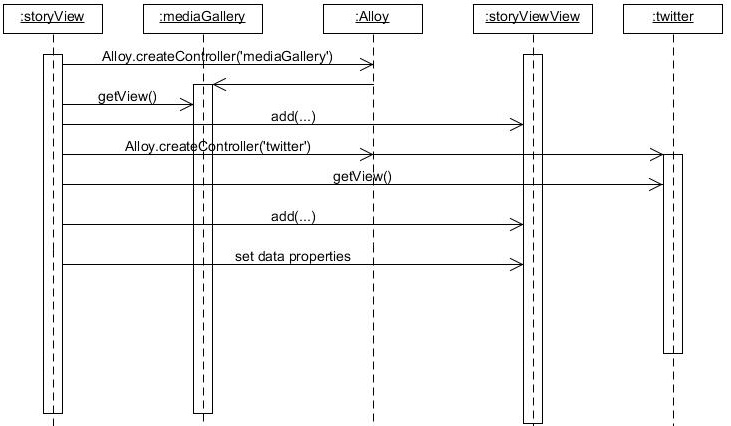
\includegraphics[width=1.0\textwidth]{Figures/Architecture/Sequence/client/storyView.jpg}
      \caption{Client - Process view for story detail view}
      \label{fig:arch_client_process_storyDetail}
\end{figure}


\subsubsection{Development view}
This view follows the description in section ~\ref{subsec:developmentViewDescription}

This is an iterative development process. In order for a function to work on the client, it must have the required support on the server. It does not mean, however, that the server must first be finished in its entirety.

\begin{figure}[H]
      \centering
      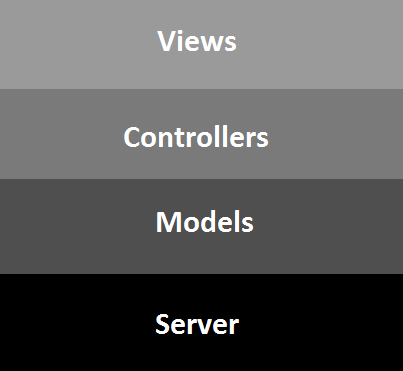
\includegraphics[width=0.5\textwidth]{Figures/Architecture/clientDevelopmentView.png}
      \caption{Client - Development view}
      \label{fig:arch_client_development}
\end{figure}

\subsection{Deployment view}
This view follows the description in section ~\ref{subsec:deploymentViewDescription}

Due to the systems being interconnected, the deployment view is made of the whole system in one diagram, instead of one for the server and anotherone for the client.

The server retrieves data from multiple services hosted on several different servers in different countries. It serves as a broker between the clients and these services.

The clients only communicate with the broker and Twitter.

\begin{figure}[H]
      \centering
      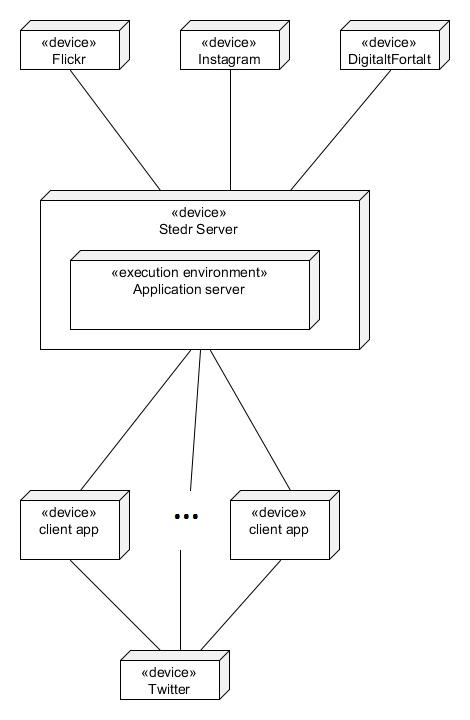
\includegraphics[width=0.8\textwidth]{Figures/Architecture/deploymentView.jpg}
      \caption{Deployment view}
      \label{fig:arch_deployment}
\end{figure}

\section{Communication interfaces}\label{sec:arch_communicationinterfaces}
Getting data from the server and by that, the services it consumes, is done by accessing a given \glspl{url} and recieving \gls{json} as a return value.

\subsection{Places}\label{placesjson}
To access the places in the system, two options are availiable.
If the objective is to get a hold of all places in the system, use the \texttt{/places.json} method, which returns a collection of all the places.

The structure of the collection can be seen in the example below.

\begin{lstlisting}[frame=single]
[
  {
    "id": "10365419324",
    "owner": "30804868@N05",
    "ownerName": "Simon Stastny",
    "title": "Atlanterhavsveien",
    "latitude": 63.016799,
    "longitude": 7.354445,
    "dateAdded": 1382204661000,
    "pictureUrl": "http:\/\/farm4.staticflickr.com\/3665\
                         /10365419324_698b0c5132.jpg",
    "thumbnailUrl": "http:\/\/farm4.staticflickr.com\/3665\
                             /10365419324_698b0c5132_t.jpg"
  },
  {
    "id": "10365389335",
    "owner": "30804868@N05",
    "ownerName": "Simon Stastny",
    "title": "Rotsethornet",
    "latitude": 62.133544,
    "longitude": 6.095094,
    "dateAdded": 1382204661000,
    "pictureUrl": "http:\/\/farm6.staticflickr.com\/5538\
                         /10365389335_6bd2a47d6b.jpg",
    "thumbnailUrl": "http:\/\/farm6.staticflickr.com\/5538\
                             /10365389335_6bd2a47d6b_t.jpg"
  }
]
\end{lstlisting}

\subsection{Places in area}
If the objective is to get only the places in a given area on the map, use the method with latitude and lingitude boundaries: \texttt{/places\_in\_area.json} with 4 parameters defining the bounding box as shown in figure~\ref{fig:arch_interface_map}: \texttt{startLatitude}, \texttt{startLongitude}, \texttt{stopLatitude} and \texttt{stopLongitude}.



When used, the query arguments should be fitted for the use case. The API assumes a Mercator-projection map like the one Google Maps are using.

Where startLongitude is the the latitude of the west (i.e. left) border of the bounding box, stopLongitude is the east (i.e. right) border, startLatitude is the south (i.e. bottom) border and stopLatitude is the north (i.e. top) border of the bounding box.

\begin{figure}[H]
      \centering
      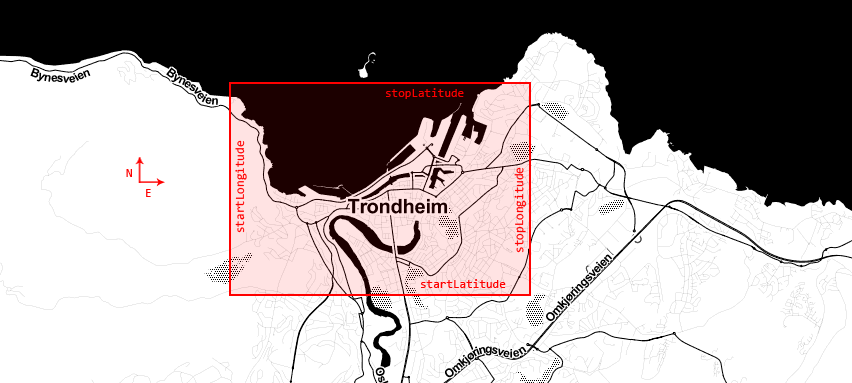
\includegraphics[width=1.0\textwidth]{Figures/Architecture/placesRange.png}
      \caption{Places in area}
      \label{fig:arch_interface_map}
\end{figure}

All latitudes and longitudes are given in \gls{dd}. To quote:

\begin{quotation}\noindent
Decimal degrees (DD) express latitude and longitude geographic coordinates as decimal fractions and are used in many geographic information systems (GIS), web mapping applications such as Google Maps, and GPS devices. Decimal degrees are an alternative to using degrees, minutes, and seconds (DMS). As with latitude and longitude, the values are bounded by $\pm$90\degree and $\pm$180\degree respectively. Positive latitudes are north of the equator, negative latitudes are south of the equator. Positive longitudes are east of Prime Meridian, negative longitudes are west of the Prime Meridian. Latitude and longitude are usually expressed in that sequence, latitude before longitude.\cite{decimalDegrees}
\end{quotation}

This means New York City has a positive latitude and negative longitude, while Rio de Janeiro has both values negative and Tokyo (or most of the Europe) both values positive.

\subsection{Stories}\label{storiesjson}
Method \texttt{http://stedr.herokuapp.com/stories.json?placeId=10357336336} returns a collection of stories in radius of 50 meters from the Place identified by the passed \textit{placeId} (which is \emph{10357336336} in this case. The structure of the collection can be seen in the example below.

\begin{lstlisting}[frame=single]
[
    {
        "author": "Kulturnett Tr\u00f8ndelag",
        "category": "Arkitektur",
        "fortelling": "\nMed utgangspunkt i Trondheim Kunstmuseum har vi fors\u00f8kt \u00e5 finne ut hva museumsarkitekturen kan fortelle oss om synet p\u00e5 kunst.\n\n",
        "ingress": "Museumsarkitektur kan fortelle s\u00e5 mangt. ",
        "institution": null,
        "language": "Norsk",
        "pictures": [
            "http://media31.dimu.no/media/image/H-DF/DF.1985/4750?height=400&width=400"
        ],
        "tags": [
            "museum",
            "funksjonalisme",
            "kunst",
            "kunstmuseum",
            "bygningshistorie",
            "modernisme",
            "Arkitektur(1)",
            "fortellerkunst",
            "Bildekunst(2)",
            "museumsutstilling",
            "museumsbes\u00f8k",
            "Kultur og samfunn(23)"
        ],
        "title": "Hva forteller museet?",
        "videos": [
            "http://mm01.dimu.no/multimedia/012MtDCo.mp4?mmid=012MtDCo"
        ]
    },
    {
        "author": "Nidaros Domkirkes Restaureringsarbeider",
        "category": "Arkitektur",
        "fortelling": "Videoen ble lagd i forbindelse med prosjektet Nordic Handscape - kulturarv i nye former - i 2005. Prosjektet skulle pr\u00f8ve ut og utvikle nye m\u00e5ter \u00e5 formidle kulturarv p\u00e5 gjennom mobil teknologi.  \nManus: Tove S\u00f8reide/NDR\nProduksjon: Klipp og Lim Media AS\nStemme: Marte Stolp\n",
        "ingress": "Videoen forteller om kalkmalingene i Regalierommet p\u00e5 Erkebispeg\u00e5rden i Trondheim. En f\u00e5r se og h\u00f8re om motivene, om maleren, og hva det hele kostet en gang i tiden. ",
        "institution": null,
        "language": "Norsk",
        "pictures": [
            "http://media31.dimu.no/media/image/H-DF/DF.1682/4136?height=400&width=400",
            "http://media31.dimu.no/media/image/H-DF/DF.1682/4135?height=400&width=400",
            "http://media31.dimu.no/media/image/H-DF/DF.1682/4138?height=400&width=400",
            "http://media31.dimu.no/media/image/H-DF/DF.1682/4137?height=400&width=400"
        ],
        "tags": [
            "nidaros",
            "embetsgardar",
            "Historie og geografi(22)",
            "kunst",
            "borger",
            "Arkitektur(1)",
            "Kulturminne(24)",
            "Bildekunst(2)",
            "kunstnere"
        ],
        "title": "Regalierommet",
        "videos": [
            "http://mm01.dimu.no/multimedia/01JY1q.mp4?mmid=01JY1q"
        ]
    }
]
\end{lstlisting}

\subsection{Images}\label{imagesjson}
Method \texttt{/images.json?tag=nidaros} returns a collection of images for the specified tag (\emph{nidaros} in this case). The structure of the collection can be seen in the example below.
\begin{lstlisting}[frame=single]
[
    {
        "fullName": "Bengt Persson",
        "url": "http://distilleryimage9.s3.amazonaws.com/05ffa296426d11e3ac5c22000ae91269_8.jpg"
    },
    {
        "fullName": "sheminbdille",
        "url": "http://distilleryimage9.s3.amazonaws.com/df08ec16422a11e395a822000ae90d43_7.jpg"
    },
    {
        "fullName": "mortensabo",
        "url": "http://distilleryimage3.s3.amazonaws.com/f8b0334a41a311e3985c22000a1f9ad3_8.jpg"
    }
]
\end{lstlisting}

\section{Architectural rationale}
Use of the Client-Server pattern ensures clean separation between the display unit and the content provider, and also helps modifiability and speed of development by providing an uniform \gls{api}.

By keeping coupeling to a minimum, the system becomes more testable and modifiable. This will help satisfy both the functional and non-functional requirements.

The Broker pattern on the server increases modifiability even though it introduces a single point of failure, but that can be mitigated by running a replica server in production.

Using the \gls{mvc} pasttern on the client provides a clean separation between logic and presentation which gives better structure to the code, increases modifiability and makes managing the code easier.

Titanium Alloy functions as a adapter between the client application and the targeted devices, and helps portability by abstracting away platform specific code where needed.

\chapter{Testing}

\begin{quotation}\noindent
Software testing is any activity aimed at evaluating an attribute or capability of a program or system and determining that it meets its required results. \cite{pan}
\end{quotation}

There are many various approaches to testing. In our project, we will perform a handful of them.

One of the approaches we are going to use is called \emph{black-box testing}. According to \cite{shinde}, this involves testing based on required functionality without knowing the implementation details and inner workings of the system. This tells us whether we implemented what we should have implemented.

Another important testing approach used in this project is \emph{white-box testing}. According to \cite{shinde}, this involves testing correctness of implemented functionality with the knowledge of the internal logic. This tells us whether the implementation is correct and works as intended. One particular instance of \emph{white-box testing} is \emph{unit testing}. This means testing individual \emph{units} (i.e. classes, modules, components) by the developer itself.

Since usability is one of our key quality requirements, we are going to perform \emph{usability tests}, as well. According to \cite{shinde}, these kinds of tests are checking the navigation of user in the system and its user friendliness.

\section{Design of test plan}

The items and the form and content of the each test document is based on the IEEE Standard 829 \cite{ieee829}. So according to the definition of test plan in the standard: ``The test plan prescribes the scope, approach, resources, and schedule of the testing activities. It identifies the items to be tested, the features to be tested, the testing tasks to be performed, the personnel responsible for each task, and the risks associated with the plan''.

\subsection{Test plan identifier}
Let this test plan to be identified as ``VirtualWall\_TESTPLAN\_1''.

\subsection{Introduction}
The Virtual Wall software system consists of two subsystems:

\begin{itemize}
    \item backend / server
    \item frontend / client (mobile / web application)
\end{itemize}

The backend is the part of the system which retrieves the data from other services and serves the frontend with the data on demand.

The client is the part of the system that presents the data to the user and that directly interacts with the user.

\subsection{Test items}
Following items shall be tested:

\begin{itemize}
    \item The source code of server subsystems will be tested.
    \item The source code of client subsystems will be tested.
    \item The user interface of the client subsystem will be tested.
\end{itemize}

\subsection{Features to be tested} \label{sec:test_plan_features_tested}
All functional requirements listed in chapter~\ref{chap:req} for this project shall be tested, unless listed as features not to be tested under section~\ref{sec:test_plan_features_not_tested}.

\subsection{Features not to be tested} \label{sec:test_plan_features_not_tested}
There are no items known to be not tested.

\subsection{Approach}
This part describes the approach taken to perform testing tasks in this project.

The overall approach is to perform a system test of all features listed under section~\ref{sec:test_plan_features_tested} using tests cases specified in section~\ref{sec:test_cases}.

During the development, the source code shall be tested using unit tests prepared by developers themselves. This simplifies the integration by making problems to be found early.

Resulting source code of both subsystems shall be tested using black-box testing. This enables us to abstract from the source code and only focus on the output and outcomes of actions, and compare this with the expected results. These tests are going to be based on test cases specified below and will be performed by black-box testers.

Apart from black-box testing, we shall perform a code inspection to assure desired quality attributes (listed in section~\ref{sec:architecture_drivers}) such as modifiability. This shall be done by white-box testers, i.e. members of the development team themselves.

All testing shall be done according to the time plan specified in the schedule table below.

Testing of the user interface shall be done by intended users of the system by means of usability testing. %FIXME SIMON: TBD usability testing

\subsection{Item pass and fail criteria}
Meeting the preconditions for each test and receiving a corresponding expected result are criteria for successful passing the test. The test is evaluated as failed otherwise.

\subsection{Test deliverables}
The documents to be delivered shall include:

\begin{itemize}
    \item \gls{srs} (System Requirements Specification)
    \item Test procedures specification (test cases)
    \item Test logs (test results)
    \item Test summary report (evaluation)
\end{itemize}

\subsection{Environmental needs}
Backend subsystem shall be deployed on a server running JRE 1.6 and able to run Play Framework!.

Server computer needs to be connected to the Internet. Specified port shall be open for server to listen on and reachable from outer network (not blocked by a firewall, etc).

Alternative setup is deploying the server to some cloud computing platform like Heroku, RedHat OpenShift, Google AppEngine, or similar. 

Device to run the client needs to be equipped Android or iOS mobile operating system. The device needs to be connected to the Internet.

\subsection{Responsibles}

The table \ref{tab:test_plan_tasks_allocation} maps responsibilities to roles in the scope of testing.

\begin{table}[H]
    \centering
    \begin{tabular}{| l | l |}
        \hline
        Task                & Responsible role              \\ \hline

        Test management     & test leader                   \\ \hline
        
        Test design         & test developers               \\
                            & test leader                   \\ \hline
        
        Test preparation    & white-box testers             \\
                            & test leader                   \\ \hline
        
        Test execution      & white-box testers             \\
                            & black-box testers             \\
                            & usability testers             \\ \hline
        
        Test evaluation     & test leader                   \\ \hline
    \end{tabular}
    \caption{Roles allocation for testing tasks.}
    \label{tab:test_plan_tasks_allocation}
\end{table}

The table \ref{tab:test_plan_roles_allocation} maps roles in testing to the members of the development team.

\begin{table}[H]
    \centering
    \begin{tabular}{| l | l |}
        \hline
        Role                & Names of allocated persons    \\ \hline

        Test leader         & Simon Stastny                 \\ \hline

        Test developers     & Christian Frøystad            \\
                            & Odd Fredrik Rogstad           \\
                            & Knut Nergård                  \\
                            & Simon Stastny                 \\ \hline

        White-box Testers   & Christian Frøystad            \\
                            & Odd Fredrik Rogstad           \\
                            & Knut Nergård                  \\
                            & Simon Stastny                 \\ \hline

        Black-box Testers   & TBD                           \\ \hline %FIXME SIMON: determine black-box testers

        Usability Testers   & TBD                           \\ \hline %FIXME SIMON: determine usability testers
    \end{tabular}
    \caption{Roles allocation for testing tasks.}
    \label{tab:test_plan_roles_allocation}
\end{table}

\subsection{Staffing and training needs}
For blackbox testing, the test responsible needs to be instructed about the system workflow in order to be able to follow the steps listed in the test cases.

For code inspection, the person performing it must have a detailed knowledge about the inner workings of the system to be able to discover possible problems and/or draw up improvements of the current solution.

For usability testing, the tester shall have (in the direction of this system) no further knowledge than what is expected to be a minimum knowledge needed for the end user to use the software . This typically includes user knowledge of computer/smartphone/tablet operations and interaction with the device (direct pointing, keyboard, or some characteristic touch gestures). Tester especially should not have an a priori knowledge about the system workflow, since this is something a typical end user will not have.
\subsection{Schedule}

The table \ref{tab:test_plan_schedule} lists tasks and maps them to people responsible for them and dates due to which they should be finished. 

\begin{table}[H]
    \centering
    \begin{tabular}{| l | l | l |}
        \hline
        Task                                & Responsible             & Due date       \\ \hline
        Design test cases for system tests  & Simon Stastny           & 2013-11-06     \\ \hline
        Design quality attribute test cases & Simon Stastny           & 2013-11-05     \\ \hline
        Design usability tests              & TBD                     & TBD            \\ \hline
        Perform black-box tests             & TBD                     & 2013-11-18     \\ \hline
        Perform usability tests             & TBD                     & TBD            \\ \hline
        Perform code inspection (server)    & Christian Frøystad      & 2013-11-05     \\ \hline
        Perform code inspection (client)    & TBD                     & TBD            \\ \hline
    \end{tabular}
    \caption{Test tasks schedule}
    \label{tab:test_plan_schedule}
\end{table}

% FIXME SIMON: fill in table

In case the functional requirements are a subject to change in the future, the design of black box tests may get delayed to absorb the changes in the requirements specification. The black box test design can only be as much finished as the functional requirement specification is.

\subsection{Risks and contingencies}

As far as we are aware, there are no risks related to testing but those mentioned in \ref{sec:project_risk_assessment} as general risks for this project.

\subsection{Approvals}

The table \ref{tab:test_plan_approvals} lists approvals of completed tasks.

\begin{table}[H]
    \centering
    \begin{tabular}{| l | l | l |}
        \hline
        Task                                & Approved by             & Date           \\ \hline
        Design test cases for system tests  & Simon Stastny           &                \\ \hline
        Design quality attribute test cases & Simon Stastny           & 2013-11-04     \\ \hline
        Design usability tests              &                         &                \\ \hline
        Perform black-box tests             &                         &                \\ \hline
        Perform usability tests             &                         &                \\ \hline
        Perform code inspection (server)    & Christian Frøystad      & 2013-11-03     \\ \hline
        Perform code inspection (client)    &                         &                \\ \hline
    \end{tabular}
    \caption{Test tasks approvals}
    \label{tab:test_plan_approvals}
\end{table}

% FIXME SIMON: fill in approvals

\section{Test levels}

\subsection{Unit test level}

\paragraph{Objective}

This level of tests is concerned about testing the correctness of implementation of individual unit (class, module, subsystem) in the system.

\paragraph{Test Environment}

To perform the tests in the unit level, we need to be able to run the unit within its subsystem. For testing units in the backend we obviously need the backend deployed on a server, etc.

\paragraph{Completion Criteria}

The unit level testing is completed when all unit tests are completed.

\paragraph{Type of Test}

This level of testing uses white-box testing since it is very important to know the application logic.


\subsection{Integration test level}

\paragraph{Objective}

This level of tests is concerned about integration of different subsystems, in this case the frontend and the backend. The purpose of tests in this level is to test the connection and cooperation of these two subsystems.

\paragraph{Test Environment}

To perform the tests in the integration level, we need both the working backend deployed on a server and a smartphone with the frontend application.

\paragraph{Completion Criteria}

The integration level testing is completed when each test is either performed or unable to be started due to unmet preconditions.

\paragraph{Type of Test}

For this level of testing, the white-box testing is to be used to find possible problems only the developers might be aware of, such as corner cases in input, etc.


\subsubsection{System Test Level}

\paragraph{Objective}

This level of tests is concerned whether the system meets the functional and technical requirements.

These tests should verify whether each function is implemented correctly and does what it is supposed to do.

\paragraph{Test environment}

For testing functionality of the backend, it must obviously be deployed on the server and running.

For testing the functionality of the frontend application, it must be running on a smartphone and connected to the internet.

\paragraph{Completion criteria}

The system level testing is completed when each test is either performed or unable to be started due to unmet preconditions.

\paragraph{Type of test}

This level of tests is concerned about the functionality. Black box method shall be used, for it is not essential to know the logic of the application code. 


\subsubsection{User Acceptance Test Level}

\paragraph{Objective}

This level of tests is usually ran by the customer on a completed product or user to find out whether the product meets all the requirement defined and it can be used in production.

Tests of this level are defined beforehand with a set of scenarios so the vendors can ran the tests themselves and find out whether the product is ready to be handed in to the customer and shipped. This is as well to ensure that a product that is known to not pass tests at the customer side is not handed in to the customer yet (to save the vendor from embarrassment and avoid waste of time).

\paragraph{Test Environment}

The test environment for this level should be as close as possible to the real-world like environment used in the production.

In our case, this means we need both the working backend deployed on a server and a smartphone with the frontend application.


\paragraph{Completion Criteria}

The user acceptance level testing is completed when each test is either performed or unable to be started due to unmet preconditions. This as well implies pass or fail result of the test respectively.


\paragraph{Type of Test}

Tests in this level shall be performed as black-box tests and usability tests. Note that we are testing real-world like usage of the system where the user is supposed to know nothing about the system and his satisfaction is very important.


\section{Test cases} \label{sec:test_cases}

This section is listing designed test cases and scenarios, that shall be used to conduct tests on the software system we developed.

\subsection{Quality attributes test scenarios}\label{sec:qatestscenarios}

Test scenarios featured in this section are designed to test the quality attributes that were chosen in section \ref{sec:req_software_system_attributes}.

\subsubsection{Modifiability scenarios}

\begin{table}[H]
  \centering
  \begin{tabular}{| l | p{11cm} |} \hline
    Source of stimulus   & Developer                                   \\ \hline
    Stimulus             & Integrate new external service              \\ \hline
    Environment          & Design time                                 \\ \hline
    Artefact             & Backend                                     \\ \hline
    Response             & New feature added                           \\ \hline
    Response measure     & Done in 5 hours                             \\ \hline
  \end{tabular}
  \caption{Quality Attribute Scenario 1}
  \label{tab:qas_newservice}
\end{table}

\begin{table}[H]
  \centering
  \begin{tabular}{| l | p{11cm} |} \hline
    Source of stimulus   & Developer                                   \\ \hline
    Stimulus             & Build application for a new platform        \\ \hline
    Environment          & Design time                                 \\ \hline
    Artefact             & Frontend                                    \\ \hline
    Response             & Application built                           \\ \hline
    Response measure     & Done in 5 hours                             \\ \hline
  \end{tabular}
  \caption{Quality Attribute Scenario 2}
  \label{tab:TC_qas_newplatform}
\end{table}

\subsection{Functional requirements test cases}

This system is featuring test cases testing the functional reuirements. These are divided into two groups by the subsystem they are testing, i.e. either backend or frontend.

\subsubsection{Backend test cases}

Test cases in \ref{tab:TCF2.2BE1}, \ref{tab:TCF3.2BE1} and \ref{tab:TCF4.1BE1} are testing the server backend part of the system. These are to be performed as white-box tests by the developers, so they can identify possible problems. This is not a function to be used directly by users.

\begin{table}
  \begin{tabular}{| p{3cm} | p{9.5cm} |} \hline 
    TC Title              & Places.json server method \\ \hline 
    TC Identification     & TC-F2.2-BE-1 \\ \hline 
    Requirement           & F2.2 \\ \hline 
    Feature               & Server exposes a method for retrieving places in the specified JSON format. \\ \hline 
    Preconditions         & \begin{enumerate}
                              \item Flickr is up.
                              \item There are some photos posted to the StedR group on Flickr that have any kind of
                               Creative Commons licence, set location and are public and visible through the Flickr API.
                              \item Server backend is successfully deployed at \texttt{http://stedr.herokuapp.com}
                            \end{enumerate} \\ \hline 

    Test description      & Manually check in browser whether the method returns the data as expected.

                            \begin{enumerate}
                              \item Open a web browser.
                              \item Go to \texttt{/places.json}
                            \end{enumerate} \\ \hline 
    Expected result       & \begin{enumerate}
                              \item The window should feature a JSON file with structure as shown in \ref{placesjson}.
                            \end{enumerate} \\ \hline 
    Pass/Fail criteria    & All results appear as expected above.
                            \begin{enumerate}
                              \item JSON file is returned and valid.
                            \end{enumerate} \\ \hline 
    Severity              & High \\ \hline 
  \end{tabular}
  \caption{Requirements Test case TC-F2.2-BE-1}
  \label{tab:TCF2.2BE1}
\end{table}


\begin{table}
  \begin{tabular}{| p{3cm} | p{9.5cm} |} \hline 
    TC Title              & Stories.json server method \\ \hline 
    TC Identification     & TC-F3.2-BE-1 \\ \hline 
    Requirement           & F3.2 \\ \hline 
    Feature               & Server exposes a method for retrieving stories for a particular place in the specified JSON format. \\ \hline 
    Preconditions         & \begin{enumerate}
                              \item Flickr is up.
                              \item Digitalt Fortalt is up.
                              \item We have a placeId from the \texttt{places.json} file (for example \texttt{10671243644})
                              \item Server backend is successfully deployed at \texttt{http://stedr.herokuapp.com}
                            \end{enumerate} \\ \hline 

    Test description      & Manually check in browser whether the method returns the data as expected.

                            \begin{enumerate}
                              \item Open a web browser.
                              \item Go to \texttt{/stories.json?placeId=10671243644}
                            \end{enumerate} \\ \hline 
    Expected result       & \begin{enumerate}
                              \item The window should feature a JSON file with structure as shown in \ref{storiesjson}.
                            \end{enumerate} \\ \hline 
    Pass/Fail criteria    & All results appear as expected above.
                            \begin{enumerate}
                              \item JSON file is returned and valid.
                            \end{enumerate} \\ \hline 
    Severity              & High \\ \hline 
  \end{tabular}
  \caption{Requirements Test case TC-F2.2-BE-1}
  \label{tab:TCF3.2BE1}
\end{table}

\begin{table}
  \begin{tabular}{| p{3cm} | p{9.5cm} |} \hline 
    TC Title              & Images.json server method \\ \hline 
    TC Identification     & TC-F4.1-BE-1 \\ \hline 
    Requirement           & F4.1 \\ \hline 
    Feature               & Server exposes a method for retrieving images for a particular tag in the specified JSON format. \\ \hline 
    Preconditions         & \begin{enumerate}
                              \item Instagram is up.
                              \item Server backend is successfully deployed at \texttt{http://stedr.herokuapp.com}
                            \end{enumerate} \\ \hline 

    Test description      & Manually check in browser whether the method returns the data as expected.

                            \begin{enumerate}
                              \item Open a web browser.
                              \item Go to \texttt{/images.json?tag=nidarosdomen}
                            \end{enumerate} \\ \hline 
    Expected result       & \begin{enumerate}
                              \item The window should feature a JSON file with structure as shown in \ref{imagesjson}.
                            \end{enumerate} \\ \hline 
    Pass/Fail criteria    & All results appear as expected above.
                            \begin{enumerate}
                              \item JSON file is returned and valid.
                            \end{enumerate} \\ \hline 
    Severity              & High \\ \hline 
  \end{tabular}
  \caption{Requirements Test case TC-F4.1-BE-1}
  \label{tab:TCF4.1BE1}
\end{table}

\subsubsection{Frontend test cases} \label{sec:fe-test-cases}

Test cases in \ref{tab:TCF2.2FE1}, \ref{tab:TCF2.2FE2}, \ref{tab:TCF3.2FE1}, \ref{tab:TCF3.2FE2}, \ref{tab:TCF3.3FE1} and \ref{tab:TCF4.1FE1} are testing the frontend part of the system. These are to be performed as black-box tests by testers, that do not need any special training or knowledge. These simulate how is the system going to be used in production, i.e. by real users.

\begin{table}
  \begin{tabular}{| p{3cm} | p{9.5cm} |} \hline 
    TC Title              & Places map overview \\ \hline 
    TC Identification     & TC-F2.2-FE-1 \\ \hline 
    Requirement           & F2.2 \\ \hline 
    Feature               & Frontend application shows a map overview with places represented as pins. \\ \hline 
    Preconditions         & \begin{enumerate}
                              \item Flickr is up.
                              \item There are some photos posted to the StedR group on Flickr that have any kind of
                               Creative Commons license, set location and are public and visible through the Flickr API.
                              \item Server backend is successfully deployed at \texttt{http://stedr.herokuapp.com} and returns data in expected format.
                              \item Frontend app is successfully installed. Device connected to the Internet.
                            \end{enumerate} \\ \hline 

    Test description      & See that the pins appear on the map in the application.

                            \begin{enumerate}
                              \item Open the frontend app.
                              \item Watch out for colored pins on the main map view.
                            \end{enumerate} \\ \hline 
    Expected result       & \begin{enumerate}
                              \item Map view should show multiple pins each representing a place.
                            \end{enumerate} \\ \hline 
    Pass/Fail criteria    & All results appear as expected above.
                            \begin{enumerate}
                              \item Places are shown.
                            \end{enumerate} \\ \hline 
    Severity              & High \\ \hline 
  \end{tabular}
  \caption{Requirements Test case TC-F2.2-FE-1}
  \label{tab:TCF2.2FE1}
\end{table}

\begin{table}
  \begin{tabular}{| p{3cm} | p{9.5cm} |} \hline 
    TC Title              & View place details \\ \hline 
    TC Identification     & TC-F2.2-FE-2 \\ \hline 
    Requirement           & F2.2 \\ \hline 
    Feature               & Frontend application shows detail of a place. \\ \hline 
    Preconditions         & \begin{enumerate}
                              \item Flickr is up.
                              \item There are some photos posted to the StedR group on Flickr that have any kind of
                               Creative Commons license, set location and are public and visible through the Flickr API.
                              \item Server backend is successfully deployed at \texttt{http://stedr.herokuapp.com} and returns data in expected format.
                              \item Frontend app is successfully installed. Device connected to the Internet.
                            \end{enumerate} \\ \hline 

    Test description      & See detail of a place (large picture, author, etc).

                            \begin{enumerate}
                              \item Open the frontend app.
                              \item Watch out for colored pins on the main map view.
                              \item Click on a pin. Bubble with place name and thumbnail appears.
                              \item Click on a bubble that appeared.
                            \end{enumerate} \\ \hline 
    Expected result       & \begin{enumerate}
                              \item Place detail view shows a large picture of the place and author of that picture, along with list of stories.
                            \end{enumerate} \\ \hline 
    Pass/Fail criteria    & All results appear as expected above.
                            \begin{enumerate}
                              \item Details are shown.
                            \end{enumerate} \\ \hline 
    Severity              & High \\ \hline 
  \end{tabular}
  \caption{Requirements Test case TC-F2.2-FE-2}
  \label{tab:TCF2.2FE2}
\end{table}

\begin{table}
  \begin{tabular}{| p{3cm} | p{9.5cm} |} \hline 
    TC Title              & View stories overview for a place \\ \hline 
    TC Identification     & TC-F3.2-FE-1 \\ \hline 
    Requirement           & F3.2 \\ \hline 
    Feature               & Frontend application shows a list of stories for a place. \\ \hline 
    Preconditions         & \begin{enumerate}
                              \item Flickr is up.
                              \item There are some photos posted to the StedR group on Flickr that have any kind of
                               Creative Commons license, set location and are public and visible through the Flickr API.
                              \item Server backend is successfully deployed at \texttt{http://stedr.herokuapp.com} and returns data in expected format.
                              \item Frontend app is successfully installed. Device connected to the Internet.
                              \item There are stories in Digitalt Fortalt related to the place.
                            \end{enumerate} \\ \hline 

    Test description      & See detail of a place (large picture, author, etc).

                            \begin{enumerate}
                              \item Open the frontend app.
                              \item Watch out for colored pins on the main map view.
                              \item Click on a pin. Bubble with place name and thumbnail appears.
                              \item Click on a bubble that appeared. Detail of place opens.
                              \item Click on \texttt{Stories} button.
                            \end{enumerate} \\ \hline 
    Expected result       & \begin{enumerate}
                              \item Overview shows tiles with stories names and pictures.
                            \end{enumerate} \\ \hline 
    Pass/Fail criteria    & All results appear as expected above.
                            \begin{enumerate}
                              \item Stories are shown.
                            \end{enumerate} \\ \hline 
    Severity              & High \\ \hline 
  \end{tabular}
  \caption{Requirements Test case TC-F3.2-FE-1}
  \label{tab:TCF3.2FE1}
\end{table}

\begin{table}
  \begin{tabular}{| p{3cm} | p{9.5cm} |} \hline 
    TC Title              & View story detail \\ \hline 
    TC Identification     & TC-F3.2-FE-2 \\ \hline 
    Requirement           & F3.2 \\ \hline 
    Feature               & Frontend application shows a detail of a story. \\ \hline 
    Preconditions         & \begin{enumerate}
                              \item Flickr is up.
                              \item There are some photos posted to the StedR group on Flickr that have any kind of
                               Creative Commons license, set location and are public and visible through the Flickr API.
                              \item Server backend is successfully deployed at \texttt{http://stedr.herokuapp.com} and returns data in expected format.
                              \item Frontend app is successfully installed. Device connected to the Internet.
                              \item There are stories in Digitalt Fortalt related to the place.
                            \end{enumerate} \\ \hline 

    Test description      & See detail of a place (large picture, author, etc).

                            \begin{enumerate}
                              \item Open the frontend app.
                              \item Watch out for colored pins on the main map view.
                              \item Click on a pin. Bubble with place name and thumbnail appears.
                              \item Click on a bubble that appeared. Detail of place opens.
                              \item Click on \texttt{Stories} button. Overview appears showing tiles with stories names and pictures.
                              \item Click on one of the pictures.
                            \end{enumerate} \\ \hline 
    Expected result       & \begin{enumerate}
                              \item Story detail view shall appear, featuring multimedia content and story text.
                            \end{enumerate} \\ \hline 
    Pass/Fail criteria    & All results appear as expected above.
                            \begin{enumerate}
                              \item Story is shown.
                            \end{enumerate} \\ \hline 
    Severity              & High \\ \hline 
  \end{tabular}
  \caption{Requirements Test case TC-F3.2-FE-2}
  \label{tab:TCF3.2FE2}
\end{table}

\begin{table}
  \begin{tabular}{| p{3cm} | p{9.5cm} |} \hline 
    TC Title              & Comment on story using Twitter \\ \hline 
    TC Identification     & TC-F3.3-FE-1 \\ \hline 
    Requirement           & F3.3 \\ \hline 
    Feature               & Frontend application shows a detail of a story. \\ \hline 
    Preconditions         & \begin{enumerate}
                              \item Flickr is up.
                              \item There are some photos posted to the StedR group on Flickr that have any kind of
                               Creative Commons license, set location and are public and visible through the Flickr API.
                              \item Server backend is successfully deployed at \texttt{http://stedr.herokuapp.com} and returns data in expected format.
                              \item Frontend app is successfully installed. Device connected to the Internet.
                              \item There are stories in Digitalt Fortalt related to the place.
                            \end{enumerate} \\ \hline 

    Test description      & See detail of a place (large picture, author, etc).

                            \begin{enumerate}
                              \item Open the frontend app.
                              \item Watch out for colored pins on the main map view.
                              \item Click on a pin. Bubble with place name and thumbnail appears.
                              \item Click on a bubble that appeared. Detail of place opens.
                              \item Click on \texttt{Stories} button. Overview appears showing tiles with stories names and pictures.
                              \item Click on one of the pictures. Story detail view appears.
                              \item Click on ``Twitter bird icon'' at the top-right corner of the screen.
                              \item Write your tweet and click on \texttt{Tweet!} button.
                            \end{enumerate} \\ \hline 
    Expected result       & \begin{enumerate}
                              \item List of twitter comments related to the place appears.
                              \item Comment is tweeted
                            \end{enumerate} \\ \hline 
    Pass/Fail criteria    & All results appear as expected above.
                            \begin{enumerate}
                              \item Twitter comments are shown.
                              \item Comment was tweeted.
                            \end{enumerate} \\ \hline 
    Severity              & High \\ \hline 
  \end{tabular}
  \caption{Requirements Test case TC-F3.3-FE-1}
  \label{tab:TCF3.3FE1}
\end{table}

\begin{table}
  \begin{tabular}{| p{3cm} | p{9.5cm} |} \hline 
    TC Title              & View pictures for a place \\ \hline 
    TC Identification     & TC-F4.1-FE-1 \\ \hline 
    Requirement           & F4.1 \\ \hline 
    Feature               & Frontend application shows pictures for a place. \\ \hline 
    Preconditions         & \begin{enumerate}
                              \item Flickr is up.
                              \item There are some photos posted to the StedR group on Flickr that have any kind of
                               Creative Commons license, set location and are public and visible through the Flickr API.
                              \item Server backend is successfully deployed at \texttt{http://stedr.herokuapp.com} and returns data in expected format.
                              \item Frontend app is successfully installed. Device connected to the Internet.
                              \item There are stories on Instagram related to the place. %FIXME related how?
                            \end{enumerate} \\ \hline 

    Test description      & See detail of a place (large picture, author, etc).

                            \begin{enumerate}
                              \item Open the frontend app.
                              \item Watch out for colored pins on the main map view.
                              \item Click on a pin. Bubble with place name and thumbnail appears.
                              \item Click on a bubble that appeared. Detail of place opens.
                              \item Click on \texttt{Pictures} button.
                            \end{enumerate} \\ \hline 
    Expected result       & \begin{enumerate}
                              \item Overview shows tiles with pictures related to the place.
                            \end{enumerate} \\ \hline 
    Pass/Fail criteria    & All results appear as expected above.
                            \begin{enumerate}
                              \item Pictures are shown.
                            \end{enumerate} \\ \hline 
    Severity              & High \\ \hline 
  \end{tabular}
  \caption{Requirements Test case TC-F4.1-FE-1}
  \label{tab:TCF4.1FE1}
\end{table}

\section{Test results and evaluation}

\subsection{Code inspection result}

\subsubsection{Backend}

Code inspection found the backend to be \emph{structured, clean, elegant, with no apparent race conditions.}.

\subsubsection{Frontend}

%FIXME SIMON: perform inspection

\chapter{Phases}
This chapter aims to document the progress of the project, but also give valuable background for decisions taken and documentation for developing against the system.

The chapter follows the outline from section~\ref{subsec:phases}, which translates to the following:
\begin{figure}[H]
    \centering
    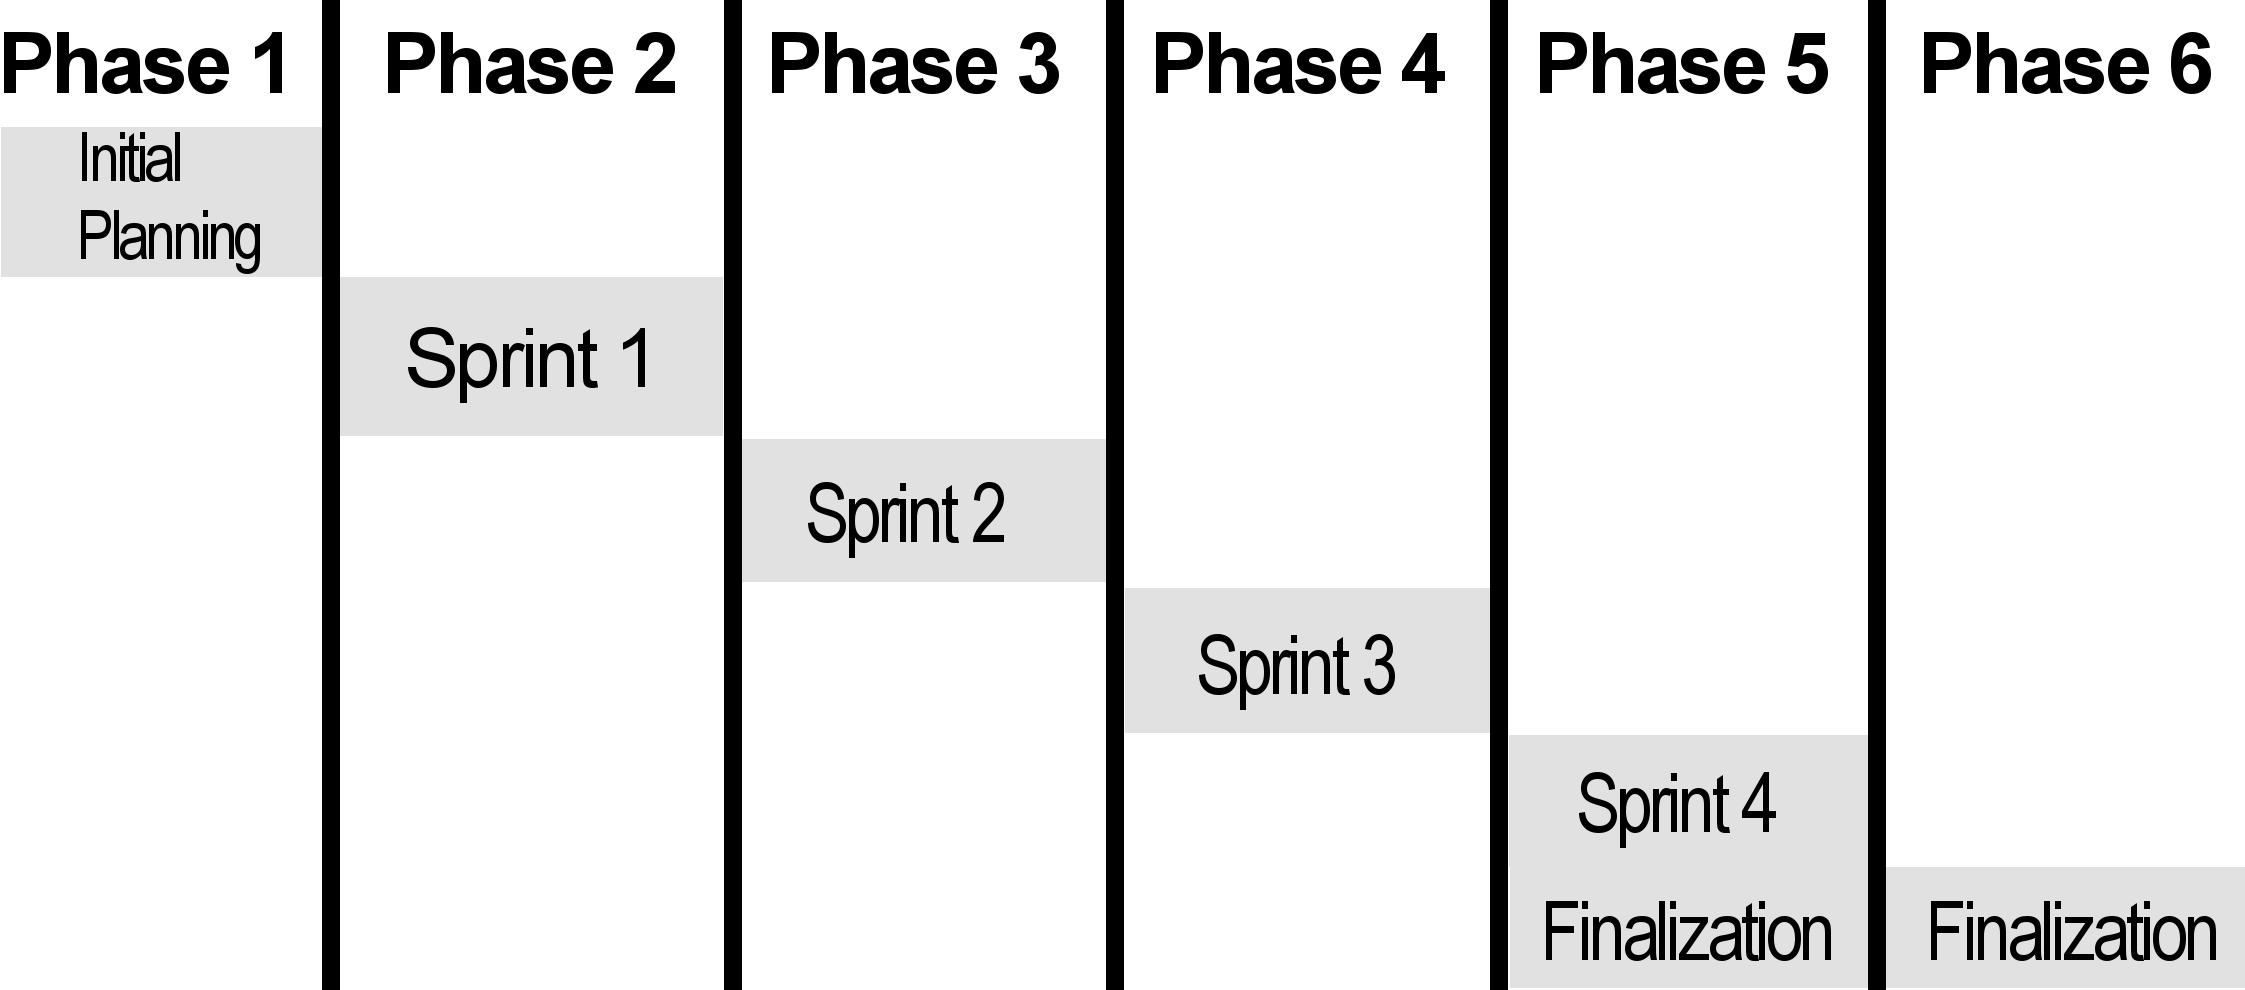
\includegraphics[width=1.0\textwidth]{Figures/Phases/phases.png}
    \caption{Chapter structure}
    \label{fig:phases_structure}
\end{figure}

\section{First phase: Planning}
The first weeks was used to get a understanding of the problem space, and how it should be solved. Chapter~\ref{chap:preliminary_study} presents the findings.

The group also focused on planning the project. The result of this can be found in chapter~\ref{chap:project_plan}.

Initial requirements was also created to get a better picture of what the system should be and how it should work. The final version can be seen in chapter~\ref{chap:req}, and the different revisions can be seen in appendix~\ref{chap:req_history}.

The groundwork of the architecture was also laid. The final document can be found in chapter~\ref{chap:architecture}.

\section{Second phase: Sprint 1}
\subsection{S1: Sprint planning}
The aim of this first sprint is to establish a baseline, in terms of technology but also with regard to the social aspects of executing a sprint as well as the amount of work being manageable within the timespan of the sprint.

\subsection{S1: Requirements as scenarios}
The server as well as the client should have a base satisfying the architectural drivers listed in \ref{sec:architecture_drivers}.

\subsection{S1: Implementation}

\subsubsection{Server}
During this period only the most basic proof of concept was developed for the server. A RESTful access point was made for the developed, with a database. All the basic groundwork was put in place, except for authentication, to develop the rest of the service.

To arrive at this proof of concept, some technological decisions had to be made. Bellow the reasoning behind them are explained.

\textbf{\gls{xmlLabel} vs \gls{json}}\\
\gls{xmlLabel} is a extensible markup language created by the World Wide Web Consortium (W3C). It is made to be both human and machine readable. It consists of a developer defined set of nested elements that may contain data or new elements.

\gls{json} \cite{json} is based on two structures: a collection of name-value pairs, and an ordered list of values. The format is made to be human readable and easily parsed and created by computers. It is based on a subset of the JavaScript programming language, and because the customer has asked for HTML5 to be used for the app \gls{json} makes sense as that will be easier to use together with JavaScript than \gls{xmlLabel}.

\textbf{\gls{rest} vs \gls{soap}}\\
\gls{rest} \cite{rest} is an architectural style that is stateless at its heart, which leads to better visibility, reliability, and scalability. \gls{rest} was developed in parallel with HTTP/1.1 and the largest system following this architectural style is the Internet (according to \cite{wikipedia:rest}). \gls{rest} is also a good match for data driven applications as the way you handle a \gls{rest} services is by utilizing the verbs GET, POST, DELETE, PUT, PATCH.

\gls{soap} is more flexible than \gls{rest}, but also much more complex. While \gls{rest} is primarily data driven through resources, \gls{soap} is logic oriented through operations. \gls{soap} is also a better choice for making stateful web services. All communication with a \gls{soap} service happens through \gls{xmlLabel}.

The simplicity of the \gls{rest} architectural style, and the fact that it allows the developer to choose the format of exchange makes this our preferred way to go.

\textbf{Play vs Spring}\\
Two of the well known frameworks when it comes to developing webservices in Java is Play! Framework and Spring. %FIXME link to websites

Spring is a very extensive framework with support for quite a few protocols and services. The framework also does a lot of work not necessarily apparent to the developer without a thorough investigation into the documentation.

The Play! Framework is more of a core framework that does the basics, but leaves it to the developer to develop the application in mostly his own style. Different from Spring, Play! Framework also reloads automatically every time a change occurs in the source, and in this way contributes to more effective development.

The extensive documentation and speed of development made us choose Play! Framework for the system.

\textbf{MySQL vs Postgres}\\
The database system most known to the developers is MySQL as this has been used in several earlier courses. Both systems are highly capable relational databases with good coverage of features and excellent performance. There are, however, particularly one issue that separates them, and make one stand out as our database of choice.

In April 2009 Oracle bought Sun \cite{sun}, and by that gained control of MySQL. Initially Oracle promised that MySQL would prevail and that it and its coming features would stay open source \cite{mysql}. The situation today shows that they have not honored that promise, and several different versions of MySQL are availiable \cite{mysqlproducts}. This serves to show that the future of MySQL is uncertain, and as such our choice falls on Postgres.

\subsubsection{Client}
The client requested use of HTML5 on the client side, so that the prototype could be tested by the whole of the test group without having to hand out phones of a specific type, but rather let the test objects use their own devices.

When it comes to real cross platform HTML5 apps, that is to say no need for native code at all, Apache Cordova is a very useful project. Apache Cordova is what was earlier known as PhoneGap \cite{phonegap}. The code was contributed to The Apache Software Foundation in 2011, at the same time Adobe acquired PhoneGaps creators Nitobi.

The way Cordova works is that it exposes native interfaces through JavaScript libraries, so that local web clients might use native features like gyroscope, accelerometer, etc. When the application is built using web technologies, it is compiled into a native webcontainer. In order to do this, one needs to have access to the platform one compiles for. For Android, you need the Android SDK. For iOS, you need an Apple computer and Xcode. For Blackberry you need WebWorks SDK.

The need for all this different platforms when building defies some of the intention of using a cross platform framework for developing the app, as it would make the workload and expenses grow quite substantially.

This is where Intel XDK comes in handy. It is a simple IDE for native web apps development with Cordova. It also includes an emulator, so that testing across units is much simplified. When ready to test on phones or build final version for deployment, Intel provides building for all platforms with a simple click in interface.

Intel also provides a fast and native looking HTML5, JavaScript and CSS library with their XDK, but due to very poor documentation for systems wishing to retain the qualities of modifiability and maintainability, the library was rejected.

Investigation into best fitted client side framework will continue into the next sprint.

\subsubsection{Interaction and user interface}
When the sprint started it was quite unclear how the application would look and feel. Within this sprint there has been two iterations on the user interface.

\textbf{Version one}\\
First thing done was to come up with what kind of main functionality the application needed;

\begin{itemize}
    \item Some kind of menu system, to navigate in the application
    \item A function to browse walls
    \item A way of displaying walls and stories
\end{itemize}

Another concern was about the definition of a wall and story, thus what kind of information did it need to display.

\textit{Menu}\\
We saw two opportunities, a dedicated menu, typically the start up point for the application, and a more hidden menu, that we'll refer to as a side-menu. The dedicated menu is typically made up with buttons, where the user can access all top-level functions. It is easy and straightforward to implement, it is also well known for most users. A more elegant solution is the hidden side-menu, where the user can access the menu wherever he or she is in the application, with just a sliding gesture from right to left on the screen.

\begin{figure}[H]
    \centering
    \includegraphics[width=0.8\textwidth]{Figures/Phases/Sprint1/versiononeSliding.png}
    \caption{Menus, dedicated vs. hidden side-menu}
    \label{fig:phases_sprint1_uiVersionOneMenu}
\end{figure}

The customer prefered the hidden side menu.

\textit{Browsing walls}\\
An important function is to let the user browse and find walls. The most obvious solutions, to use a map and/or a list, were discussed, but no solution was determined. 

Another important function is to filter or sort the walls. In a list it is easy to sort the walls on, for instance, popularity or the distance to your location using GPS tracking. There were suggested to use some kind of temperature pins in a map, where the pins shows the user how popular the different places are by using colors. The user could also decide to only see the most popular places by excluding the more cold colored walls, as Figure~\ref{fig:phases_sprint1_uiVersionOneTempPings} shows. The temperature pins were just one of many suggestion on how to represent walls on a map, others where to use symbols or icons, one colored pins and images.

The customer wanted to focus more on the use of filtering on tags and metadata.

\begin{figure}[H]
    \centering
    \includegraphics[width=0.8\textwidth]{Figures/Phases/Sprint1/versiononeTempPings.png}
    \caption{Temperature pins, with filtering}
    \label{fig:phases_sprint1_uiVersionOneTempPings}
\end{figure}

\textit{Look at walls}
The main function of the application is to access a wall and browse user created information, that could be stories, pictures, links to other resources, etc.. Two possible solution were suggested; a wall that displayed both user created stories and information from multiple data sources as in Figure~\ref{fig:phases_sprint1_uiVersionOneSimpleWall}, for instance, Instagram, Wikipedia, YouTube, Twitter, Google, Flickr, etc., and a more simple version where the focus was on user created data, thus stories and pictures, as in Figure~\ref{fig:phases_sprint1_uiVersionOneMultipleDataSoruces}.

The idea of using multiple data sources came from the danish mobile application, \emph{Kulturarv}, or \emph{Cultural Heritage} (both mentioned in \ref{sec:prestudy_existing_apps}), which blends data from a main database with other geo location data sources like Instagram, Flickr, Wikipedia and Twitter. The customer had not thought about the idea of using multiple data sources, and were therefore quite surprised by the solution. The group and customer agreed that the use of multiple data sources were out of the scope, and decided to focus on the more simple version. The customer liked the use of tabs, to navigate, within a wall.

\begin{figure}[H]
    \centering
    \includegraphics[width=0.8\textwidth]{Figures/Phases/Sprint1/versiononeSimpleWall.png}
    \caption{Simple wall, with tabs to navigate. Nidarosdomen is used as an example}
    \label{fig:phases_sprint1_uiVersionOneSimpleWall}
\end{figure}

\begin{figure}[H]
    \centering
    \includegraphics[width=0.8\textwidth]{Figures/Phases/Sprint1/versiononeMultipleDataSourcesWall2.png}
    \caption{Wall using multiple data sources, with slide gestures to navigate. Nidarosdomen is used as an example}
    \label{fig:phases_sprint1_uiVersionOneMultipleDataSoruces}
\end{figure}

\textbf{Version two}\\
In this iteration the focus was on how to filter walls on tags, how to switch between list or map browsing, how to create a wall and on the wall itself. 

\textit{Filtering walls}\\
The customer wanted the user to filter by tags, both on tags that was suggested to the user and tags that the user typed himself. A suggested solution is shown in Figure ~\ref{fig:phases_sprint1_uiVersionTwoAddFilter}. The customer found the solution satisfactory, but the user also needed to be able to filter on creators of walls. It was suggested to introduce the @-sign to filter on creators.

\textit{List or map browsing}\\
Three possible solutions were made, one with tabs, one with action buttons and one with a drop down menu (Figure ~\ref{fig:phases_sprint1_uiVersionTwoAccessListOrMap}). The customer dropped the whole proposal, and wanted just to use map when browsing walls.

\begin{figure}[H]
    \centering
    \includegraphics[width=0.8\textwidth]{Figures/Phases/Sprint1/accessListOrMap.png}
    \caption{How to switch between list or map browsing}
    \label{fig:phases_sprint1_uiVersionTwoAccessListOrMap}
\end{figure}

\begin{figure}[H]
    \centering
    \includegraphics[width=0.8\textwidth]{Figures/Phases/Sprint1/addFilter.png}
    \caption{Filtering on tags}
    \label{fig:phases_sprint1_uiVersionTwoAddFilter}
\end{figure}

\textit{Create wall}\\
This function is very important, because it will define the the definition of a wall, thus the content of a wall. The customer wanted a more purified story-telling-wall, a wall that tells stories. The proposal was that a wall would consist of a title, a description, a set of tags, a gallery, stories and a location. The possibility to let everyone add content and to comment were also a part of the solution, as Figure ~\ref{fig:phases_sprint1_uiVersionTwoCreateWallDocument} shows.

\begin{figure}[H]
    \centering
    \includegraphics[width=0.8\textwidth]{Figures/Phases/Sprint1/createWallDocument.png}
    \caption{Create wall}
    \label{fig:phases_sprint1_uiVersionTwoCreateWallDocument}
\end{figure}

\textit{The wall}\\
From version one we knew that the customer wanted a wall that was focused on the user created data, stories and images. A solution, the one in Figure ~\ref{fig:phases_sprint1_uiVersionTwoWallFunctions}, were suggested. The wall uses tabs for navigation, and the solution included two suggestions for displaying stories, a list and tiles. The customer liked the solution, and decided to use tiles to represent stories.

\begin{figure}[H]
    \centering
    \includegraphics[width=0.8\textwidth]{Figures/Phases/Sprint1/wallFunctions.png}
    \caption{The wall}
    \label{fig:phases_sprint1_uiVersionTwoWallFunctions}
\end{figure}

\subsection{S1: Test execution}
This sprint no formal testing was done, only functional tests on the server and discussions around the user interface.

\subsection{S1: Review}
We did not manage to finish all the predefined tasks for this sprint. This was partly due to the absence of two group members during most of the sprint period. The delay was also partly due to inexperience with mobile JavaScript frameworks and the lack of real documentation for most of them.

\section{Third phase: Sprint 2}
\subsection{S2: Sprint planning}
The goal of the second sprint was initially to build upon the bases put in place by sprint one, but due to a steep learning curve in JavaScript and lack of real documentation for most frameworks this was not the case.

The server has seen development based upon what was done in sprint one, but the client has started from scratch.

\subsection{S2: Backlog}
\begin{table}[H]
    \centering
    \begin{tabular}{| l | l |} \hline
        Item                                                                & Outcome         \\ \hline
        Define the concept of story                                         & Done            \\ \hline
        Define the main principles of UI                                    & Done            \\ \hline
        Browse virtual walls                                                & Done in server  \\ \hline
        Open a virtual wall                                                 & Done in server  \\ \hline
        Basic framework for app with support for communicating with server  & Done            \\ \hline
        Architecture                                                        & Partly done     \\ \hline
    \end{tabular}
    \caption{Backlog for sprint 2.}
    \label{tab:phase_sprint2_backlog}
\end{table}

\subsection{S2: Requirements as scenarios}
\textbf{Browse virtual walls}
\begin{enumerate}
    \item User goes to map view
    \item Client asks user for location
    \item User write location or taps on fetch my location
    \item Map shows the users position
    \item Walls are indicated on the map
    \item The user might move around in the map by dragging it around
\end{enumerate}

\textbf{Open a virtual wall}
\begin{enumerate}
    \item User goes to walls view (that be map or list or whatever is decided)
    \item User navigates to wall of interest - see [wall browsing] Browse virtual walls
    \item User taps on desired wall
    \item Client shows a new screen with the wall content
\end{enumerate}

\subsection{S2: Implementation}

\subsubsection{Definition of story}
A story is defined by its existance on Digitalt Fortalt, and thus uses Digitalt Fortalts definition of a story.

\subsubsection{Server}

In this sprint the requirements for the overall workings of the system seemed to be somewhat stable so we designed a data model and implemented it on the server side. This turned out to be a wrong assumption later on.

\subsubsection{Client}
\textbf{Sync client}\\
Titanium Alloy is backend agnostic. This means that most of the code does not know, nor need to know, what kind of backend is running. This is accomplished by utilizing an abstraction layer in Alloy called Sync. Sync provides an unified API that can be implemented for each type of backend.\\
The API has the following methods:

\begin{table}[H]
    \centering
    \begin{tabular}{| p{3.5cm} | p{3.5cm} | p{3.5cm} | p{2.5cm} |}
        \hline
        Backbone Method & Sync CRUD Method & Equivalent \gls{http} Method & Equivalent \gls{sql} Method\\
        \hline
        Collection.fetch & read & GET & SELECT\\
        \hline
        Collection.create (id == null) or Collection.create (id != null) & create or update & POST or PUT & INSERT or UPDATE\\
        \hline
        Model.fetch & read    & GET & SELECT\\
        \hline
        Model.save (id == null) or Model.save (id != null) & create or update & POST or PUT & INSERT or UPDATE\\
        \hline
        Model.destroy & delete & DELETE & DELETE\\
        \hline
    \end{tabular}
    \caption{API for Sync in Alloy\cite{titaniumAlloySync}}
    \label{tab:phase_sprint2_model}
\end{table}

As the application makes use of \gls{rest} server, a backend supporting \gls{rest} was needed. Although a custom backend could have been created, it made more sense to reuse the implementation of others. The \texttt{napp.alloy.adapter.restapi}\footnote{https://github.com/viezel/napp.alloy.adapter.restapi} by Mads Møller was chosen due to its feature completeness and active development.

\textbf{Models}\\
Models in Titanium Alloy build upon Backbone.js\footnote{http://backbonejs.org/} \cite{titaniumAlloyModel}. Therefor the documentation for Backbone.js is relevant in addition to the documentation from Titanium.

A basic model looks like this:
\begin{lstlisting}[frame=single]
exports.definition = {
    config : {
        "columns" : {
            "wallId" : "int",
            "name" : "string",
            "description" : "string",
            "latitude" : "double",
            "longitude" : "double",
        },
        "URL" : "http://stedr.herokuapp.com/walls.json",
        "adapter" : {
            "type" : "restapi",
            "collection_name" : "wall",
            "idAttribute" : "wallId"
        }
    },
    extendModel : function(Model) {
        _.extend(Model.prototype, {
            // If adding and editing walls shall be allowed,
            // the specific url must be added here
        });
        return Model;
    },
    extendCollection : function(Collection) {
        _.extend(Collection.prototype, {});
        return Collection;
    }
};
\end{lstlisting}

Before choosing Titanium as the platform to develop the client application with, a number of other frameworks were examined.

\textbf{The M project}\\
Initially “The M project” \footnote{http://www.the-m-project.org/} came out quite good in comparisons of frameworks for client side development for mobile phones. This was due to it being lightweight and what seemed like usable documentation. Its described caracteristica also matched quite good with what we was looking for. Especially the \gls{mvc} part and the native look and feel of the jQuery Mobile user interface. The MIT license was also very attractive, as it is compatible with the BSD license required for all code produced in this course.

The reasons why The M project was not chosen in the end, surrounds two topics. First, the project has its own build system to help the developers develop more efficiently. Unfortunately this did not work, and produced unrunnable code. One could edit the files after each build in order to make them runnable, but 5 minutes extra per build to clean the code was just not acceptable.

The second problem is of a more serious kind, both for this development team and for those that might follow at a later time. The documentation was vague at best and partly outdated.

\textbf{Enyo}\\
Enyo\footnote{http://enyojs.com/} was developed by HP for WebOS\cite{enyoHistory} and is at this time sponsored by LG. It has a very interesting approach to development, one develops features in the app as separate reusable components and glue them together. In that way it feels much more natural to develop in Enyo, and the documentation is excellent. The license, Apache 2.0, is also very attractive as it is compatible with BSD.

The problem with Enyo was that the requirements specified modifiability as one very important factor to take into account. While components can make the app itself modifiable, Enyo does not support \gls{mvc} in the components and as such one just moves the complexity one level down. When developing components we would still have to handle that lack of ability to structure the code in an efficient way.

Adding support for \gls{mvc}, or making it easy to use \gls{mvc} in combination with the rest of the framework, is an ongoing effort at Enyo.

The reason Enyo was not selected is that the \gls{mvc} support has not yet stabilized, and the documentation is still a bit too thin on the matter.

\textbf{Sencha Touch}\\
Sencha Touch\footnote{http://www.sencha.com/products/touch/} has excellent documentation and a good community. The problem with Sencha is the incompatible license. Sencha uses the General Public License version 3, which is incompatible with the BSD license.\cite{flossLicense}

\textbf{RhoMobile}\\
RhoMobile is developed by Motorola Solutions\footnote{http://www.motorolasolutions.com/US-EN/Business+Product+and+Services/Software+and+Applications/RhoMobile+Suite} to help developers develop software across their different handheld devices. They have also added support for the mobile platforms. This framework has support for developing enterprise applications and has an attractive license in MIT.
The reason this framework was not chosen, was because it uses Ruby as well as JavaScript. It was decided that learning one new language would be enough work, if not another one should be added on top.

\textbf{Titanium}\\
Appcelerator Titanium\footnote{http://www.appcelerator.com/titanium/} is a cross platform development framework for mobile and web. The development is done in JavaScript and \gls{xmlLabel}. It is licensed under the Apache Public License version 2. Titanium is a ``write once, adapt everywhere'' framework\cite{titaniumCrossMobile}. That does not mean that it cannot run everywhere without adaption, but that in order to look native it needs adaption. Titanium has an excellent base of documentation and a mature framework supporting easy use of the model view controller architectural pattern.

Titanium was chosen because of its framework, its documentation and the huge community that surrounds it.


\subsection{S2: Test execution}
Only functional testing was done for this sprint as development went on. No systematic testing was executed.

\subsection{S2: Review}
Once again we would like to have reached a milestone farther ahead at this time, but we have had to spend a lot more time learning new mobile frameworks than we had expected. 

Nevertheless, the group has seen increased participation during this sprint, and more group members has become more active. This has lead to us getting more done than in the earlier sprints, and we how this will also mean that we will get even more done in the coming sprints.

Some of our goals for this sprint was only reached for the server. The reason for this is the fact that the group members are more accustomed to Java than JavaScript, and the fact that Play! Framework has better documentation available than the mobile frameworks we have used.

The architecture is only partially done, this is due to the change in mobile framework and requirements. Now that a mobile framework has been chosen and the requirements more stabilized, we hope to have the architecture finished within a relatively short amount of time.

\section{Fourth phase: Sprint 3}
\subsection{S3: Sprint planning}
\subsection{S3: Backlog}
\begin{table}[H]
    \centering
    \begin{tabular}{| l | l |} \hline
        Item                                                                & Outcome         \\ \hline

    \end{tabular}
    \caption{Backlog for sprint 3.}
    \label{tab:phase_sprint3_backlog}
\end{table}

\subsection{S3: Requirements as scenarios}

\subsection{S3: Implementation}

\subsubsection{Server}

Upon receiving changes proposed by customer, the data model was stashed and reworked to accommodate the proposed changes. As the concept of walls and stories finally settled down, we were able to implement API for retrieving walls based on geographic coordinates and to retrieve stories on walls.

As requested in the last batch of change requests from customer, stories shall be stored in an external database called \emph{Digitalt Fortalt}. This database provides an API for search which we call to retrieve the stories. Our application does not write any data to \emph{Digitalt Fortalt}, stories need to be created manually on their website.

Walls on the other hand shall be stored in out system database. We now store each wall with its geographic coordinates in a database table and filter as described in \ref{sec:spr3_maps}. 

Data stored in our database are retrieved by classes in the \texttt{models} package. The models are extending \texttt{play.db.ebean.Model} class and use standard \gls{jpa} annotations to indicate relationships between entities.

The data from \emph{Digitalt Fortalt} are retrieved from the API by classes in the \texttt{retrievers} package. The data are fetched and parsed by using the \emph{jsoup} Java \gls{html} parser. We found this library to be more usable than \emph{DOM} and \emph{SAX} parser implementations in Java (due to various reasons such as usage of \texttt{Iterable} interface, which make the work with collection-like structures much easier).

\subsubsection{Map views, coordinates and projections} \label{sec:spr3_maps}

One of the main features of the application is to show user location of various virtual walls on a map. Since we decided to use Titanium framework for the development of the mobile application, we are using its own map view (\texttt{Titanium.Map.View}) for the display of maps and locations of walls upon them.

The database is now featuring just a few walls, but it is supposed to host much more of them in the future and it would not be optimal for the performance and operational reasons (such as costs of data transfers on mobile Internet) to fetch all the walls when user is using the application.

The user is only interested in walls he could actually see on the map, so we decided to take an approach where we fetch the data from the server while filtering it upon geographic coordinates. The map view supplies us with a geographical coordinates of the center of the displayed map and with west-to-east distance and noth-to-south distance. This makes it possible to compute the coordinates of the north-west (i.e. top-left) corner of the map view, and the south-east (i.e. bottom-right) corner of the map view. Then the application fetches the data from the server, asking it to filter only those walls, which have coordinates in the rectangle defined by those two corners.

It is a well-known fact that planet Earth is not flat. For this reason, various map projections are used to transform the surface of Earth (3D) onto a plane (2D). Google Maps, which provide the map tiles for the map view, are using a variant of so called Mercator \footnote{Named after Flemish geographer and cartographer Gerardus Mercator, who firstly used it in 1569 for his map titled \emph{Nova et Aucta Orbis Terrae Descriptio ad Usum Navigantium Emendate Accommodata}, which is Latin for \emph{New and more complete representation of the terrestrial globe properly adapted for use in navigation}.} projection. This map projection was used in naval navigation for showing constant bearings (\emph{loxodromes}, also known as \emph{rhumb lines}) as straight lines on the map. \cite{progonos:mercator,radicalcartography} 

\begin{figure}[H]
    \centering
    \includegraphics[width=0.8\textwidth]{Figures/Prestudy/mercator.png}
    \caption{Mercator cylindrical map projection basics. \cite{wikipedia:mercator}}
    \label{fig:mercator}
\end{figure}

As seen in \ref{fig:mercator}, it is a cylindrical conformal projection, so it preserves local angles, but is unfit for use in high-latitudes as the map extends infinitely North and South (so called \emph{polar exaggeration}). This shall be fine for use until we need to add a wall for a location near to one of the geographic poles (which are stretched infinitely along the top and bottom edges of the map). This could be a problem is we want to add a wall for example for the Amundsen–Scott South Pole Station located just few meters from the geographical such pole and which would and stretch widely east to west. \cite{progonos:mercator,radicalcartography} 


\subsection{S3: Test execution}
\subsection{S3: Review}
\subsection{S3: Phase evaluation}

\section{Fifth phase: Sprint 4}

\subsection{S4: Sprint planning}
The project plan states that there are to be 4 sprints, and that the last one (Sprint 4) will start on october 23rd. and last until november 11th. This leaves two weeks for finalizing the report and a presentation.

Ideally this would be the prefered route, but due to the projects current status some changes needs to be made. Four persons working 50 hours or more each on making finishing touches on a document and a presentation is quite extensive, given the fact that the system still needs quite some work.

Sprint 4 is therefor extended with one week. It will last from 23.10.2013 - 13.11.2013, amounting to three weeks.

During Sprint 4 one person is allocated to fix any issues with the report, so that in the last phase (finalization) the group might focus solely on the presentation and proof reading.

In Sprint 4, the group should also place an emphasis on testing, as very little has formally been done in that regard earlier in the process.

\textbf{Allocation matrix}\\
\begin{table}[H]
    \centering
    \begin{tabular}{| l | l | l | l |} \hline
         & App & Testing & Report\\
         \hline
         Odd & 3 weeks & 0 & 0\\
         \hline
         Simon & 2 weeks & 1 week & 0\\
         \hline
         Knut & 2 weeks & 1 week & 0\\
         \hline
         Christian & as needed & 1 week & 2 weeks\\
         \hline
    \end{tabular}
    \caption{Allocation matrix for sprint 4}
    \label{tab:phase_sprint4_allocation}
\end{table}


\subsection{S4: Backlog}
\begin{table}[H]
    \centering
    \begin{tabular}{| l | l |} \hline
        Item                                                                & Outcome         \\ \hline
        Define the main principles of UI & Done\\
        \hline
        Finish system architecture & Done\\
        \hline
        Browse virtual walls - retrieve picture(s) from flickr & Done\\
        \hline
        Open a virtual wall & Done\\
        \hline
        Create virtual wall & Done\\
        \hline
        Open story & Done\\
        \hline
        Add story to wall & \\
        \hline
        Filter stories by tags & \\ 
        \hline
        Adding instagram information related to a wall  & \\
        \hline
        Retrieving instagram information related to a wall & \\
        \hline
        Add comment to a story & Done\\
        \hline
    \end{tabular}
    \caption{Backlog for sprint 4.}
    \label{tab:phase_sprint4_backlog}
\end{table}

\subsection{S4: Requirements as scenarios}
\subsubsection{Create virtual wall}
\begin{enumerate}
\item User goes to map view
\item User taps on the add icon (a plus sign)
\item System provides user with information about how to add a new wall
\end{enumerate}

\subsubsection{Add story to wall}
\begin{enumerate}
\item User goes to story view on a wall
\item User taps on the add icon (a plus sign)
\item System provides user with information about how to add a new story
\end{enumerate}

\subsubsection{Filter stories by tags or author}
\begin{enumerate}
\item User goes to the story view of a wall
\item User pulls out tags panel and selects desired tags by browsing or searching
\item Client fetches stories from server that matches the chosen tags
\item Tags panel disappear and wall view is updated with only stories matching the tags
\end{enumerate}

\subsubsection{Browse stories}
\begin{enumerate}
\item User opens a wall
\item User navigates to stories tab
\item User navigates the tiles by dragging and tapping
\end{enumerate}

\subsubsection{Open story}
\begin{enumerate}
\item User navigates to a wall
\item User browses stories
\item User selects a desired story by tapping on it
\item Client displays the story
\end{enumerate}

\subsection{S4: Implementation}

\subsubsection{Client}
\textbf{Instagram}\\
Instagram API does not support fetching of several tags simultaneously.
Instagram has a limit of 30 pictures to be shown per page. 
Can be problematic, legally, to show all pictures without filtering by humans.

subsubsection{Server}

\subsection{S4: Test execution}
To be written
\subsection{S4: Review}
To be written
\subsection{S4: Phase evaluation}
To be written

\section{Last phase: Finalization}
To be written

\chapter{Evaluation of the project}
To be written

\bibliography{bibliography}

\appendix
\chapter{Initial project description from customer}
The following description is taken from the course compendium\cite[p. 47]{compendium}.

\begin{quotation}\noindent
The assignment relates to the EU-IST project TAG CLOUD (www.tagcloudproject.eu). TAG CLOUD will develop innovative digital solutions with the aim to increase the engagement of people in culture and cultural heritage. The main aspects that will be investigated are: new interaction interfaces with cultural artifacts, user as a contributor and personalized information. In Norway, the focus is ``culture in the landscape'', i.e. the discovery of cultural memories that we meet when walking around in cities, in villages and in the nature.

The goal of this assignment is to develop a tool to create and interact with ``virtual walls''. The idea stems from Væggen\footnote{Væggen is the danish word for ”Wall”.} in Copenhagen (http://vaeggen.copenhagen.dk/dk/). Væggen is a large multitouch screen allowing people to tell, share and experience stories. We would like to explore the concept of wall as means to discover and share cultural stories related to buildings and places. It is however not practical to install and maintain physical walls such as Væggen all around. Instead we propose a digital representation of walls, that we call virtual wall.

The assignment will build upon interactive pictures for the realization of virtual walls. The tool that will be develop should include support for:
\begin{itemize}
    \item Managing virtual walls: creation/deletion; retrieval according to location, popularity, topics and other metadata (e.g. author)
    \item Managing stories: adding stories through a click on a specific place on the wall, filtering stories
according to popularity, topics and other metadata (e.g. duration)
    \item Social interaction: sharing walls (possibly stories) for editing, adding comments to walls and stories.
    \item Promotion through social networks: sharing walls and stories through social networks (e.g. Facebook, Twitter)
\end{itemize}
The tool should be available for PC, tablet and mobile allowing experience at home and on site. The assignment should specify a system architecture that fits this requirement and select technologies that simplify development on several platforms. The assignment will realized the tool for one device type, preferably tablet.

The tool thinglink (http://www.thinglink.com) supports some of the proposed functionality, but we wish to go further. In particular, the dynamic generation of a wall is needed for the filtering of stories. Our ultimate goal is to connect the wall with the personalization back-end that will be developed in TAG-CLOUD allowing to provide recommendations to the users.

More information: As an example, we have started to develop a draft wall for Nidarosdomen using thinglink (http://www.thinglink.com/scene/397385278152507392). A presentation is also available at https://www.dropbox.com/l/GjCOoSqHoAmMEGg6P0axxa

Additional notes: All documentation (report and code comments) should be written in English. The results should be made open source.\cite[p. 47]{compendium}
\end{quotation}

\chapter{Timesheets}
\begin{table}[H]
\centering
\begin{tabular}{| l | l | l | l | l | l | l | l |}
    \hline
    Group total         &             &             &             &             &             &             &                 \\ \hline                        
    Activity/Period     & Phase 1     & Phase 2     & Phase  3    & Phase 4     & Phase 5     & Phase 6     & Activity sum    \\ \hline
    Lectures/self study & 48:15    & 2:45     & 37:45    & 24:00    & 0           & 0           & 112:45       \\ \hline
    Admin               & 35:30    & 30:00    & 23:50    & 32:15    & 0           & 0           & 121:35       \\ \hline
    Planning            & 26:05    & 0:00     & 3:00     & 0:00     & 0           & 0           & 29:05        \\ \hline
    Pre-study           & 45:10    & 23:30    & 29:15    & 17:30    & 0           & 0           & 115:25       \\ \hline
    Requirements        & 16:30    & 4:30     & 0:00     & 1:30     & 0           & 0           & 22:30        \\ \hline
    Implementation      & 0:00     & 0:50     & 10:30    & 140:10   & 0           & 0           & 151:30       \\ \hline
    Design              & 3:45     & 23:10    & 9:00     & 5:00     & 0           & 0           & 40:55        \\ \hline
    Testing             & 0:00     & 0:00     & 10:00    & 0:00     & 0           & 0           & 10:00        \\ \hline
    Documentation       & 2:30     & 5:30     & 14:30    & 11:50    & 0           & 0           & 34:20        \\ \hline
    Period sum          & 177:45   & 90:15    & 137:50   & 232:15   & 0           & 0           & 638:05       \\ \hline
\end{tabular}
\caption{Time sheet for group as total}
\label{tab:appendix_timesheets_group}
\end{table}

\begin{table}[H]
\centering
\begin{tabular}{| l | l | l | l | l | l | l | l |}
    \hline
    Rogstad             &             &             &             &             &             &             &                 \\ \hline                        
    Activity/Period     & Phase 1     & Phase 2     & Phase  3    & Phase 4     & Phase 5     & Phase 6     & Activity sum    \\ \hline
    Lectures/self study & 12:15    & 0:00     & 14:00    & 4:00     & 0           & 0           & 30:15        \\ \hline
    Admin               & 13:45    & 8:45     & 6:45     & 7:45     & 0           & 0           & 37:00        \\ \hline
    Planning            & 0:00     & 0:00     & 0:00     & 0:00     & 0           & 0           & 0:00         \\ \hline
    Pre-study           & 21:00    & 17:45    & 16:15    & 2:00     & 0           & 0           & 57:00        \\ \hline
    Requirements        & 0:00     & 0:00     & 0:00     & 0:00     & 0           & 0           & 0:00         \\ \hline
    Implementation      & 0:00     & 0:00     & 0:00     & 52:15    & 0           & 0           & 52:15        \\ \hline
    Design              & 0:00     & 0:00     & 0:00     & 0:00     & 0           & 0           & 0:00         \\ \hline
    Testing             & 0:00     & 0:00     & 0:00     & 0:00     & 0           & 0           & 0:00         \\ \hline
    Documentation       & 0:00     & 0:00     & 0:00     & 0:00     & 0           & 0           & 0:00         \\ \hline
    Period sum          & 47:00    & 26:30    & 37:00    & 66:00    & 0           & 0           & 176:30       \\ \hline
\end{tabular}
\caption{Time sheet for Odd Fredrik Rogstad}
\label{tab:appendix_timesheets_odd}
\end{table}

\begin{table}[H]
\centering
\begin{tabular}{| l | l | l | l | l | l | l | l |}
    \hline
    Frøystad            &             &             &             &             &             &             &                 \\ \hline            
    Activity/Period     & Phase 1     & Phase 2     & Phase  3    & Phase 4     & Phase 5     & Phase 6     & Activity sum    \\ \hline
    Lectures/self study & 15:30    & 0:30     & 10:45    & 4:00     & 0           & 0           & 30:45        \\ \hline
    Admin               & 14:15    & 16:15    & 13:35    & 17:00    & 0           & 0           & 61:05        \\ \hline
    Planning            & 24:05    & 0:00     & 3:00     & 0:00     & 0           & 0           & 27:05        \\ \hline
    Pre-study           & 11:40    & 3:30     & 10:00    & 5:00     & 0           & 0           & 30:10        \\ \hline
    Requirements        & 0:00     & 0:00     & 0:00     & 0:00     & 0           & 0           & 0:00         \\ \hline
    Implementation      & 0:00     & 0:50     & 2:00     & 12:55    & 0           & 0           & 15:45        \\ \hline
    Design              & 3:45     & 23:10    & 8:00     & 4:00     & 0           & 0           & 38:55        \\ \hline
    Testing             & 0:00     & 0:00     & 0:00     & 0:00     & 0           & 0           & 0:00         \\ \hline
    Documentation       & 0:00     & 0:00     & 0:00     & 7:50     & 0           & 0           & 7:50         \\ \hline
    Period sum          & 69:15    & 44:15    & 47:20    & 50:45    & 0           & 0           & 211:35       \\ \hline
\end{tabular}
\caption{Time sheet for Christian Frøystad}
\label{tab:appendix_timesheets_christian}
\end{table}

\begin{table}[H]
\centering
\begin{tabular}{| l | l | l | l | l | l | l | l |}
    \hline
    Stastny             &             &             &             &             &             &             &                 \\ \hline          
    Activity/Period     & Phase 1     & Phase 2     & Phase  3    & Phase 4     & Phase 5     & Phase 6     & Activity sum    \\ \hline
    Lectures/self study & 8:15     & 0:00     & 2:00     & 4:00     & 0           & 0           & 14:15        \\ \hline
    Admin               & 4:45     & 3:30     & 3:30     & 4:00     & 0           & 0           & 15:45        \\ \hline
    Planning            & 0:00     & 0:00     & 0:00     & 0:00     & 0           & 0           & 0:00         \\ \hline
    Pre-study           & 7:30     & 0:00     & 0:00     & 1:00     & 0           & 0           & 8:30         \\ \hline
    Requirements        & 16:30    & 4:30     & 0:00     & 1:30     & 0           & 0           & 22:30        \\ \hline
    Implementation      & 0:00     & 0:00     & 7:00     & 65:30    & 0           & 0           & 72:30        \\ \hline
    Design              & 0:00     & 0:00     & 0:00     & 0:00     & 0           & 0           & 0:00         \\ \hline
    Testing             & 0:00     & 0:00     & 10:00    & 0:00     & 0           & 0           & 10:00        \\ \hline
    Documentation       & 0:00     & 0:00     & 14:30    & 4:00     & 0           & 0           & 18:30        \\ \hline
    Period sum          & 37:00    & 8:00     & 37:00    & 80:00    & 0           & 0           & 162:00       \\ \hline
\end{tabular}
\caption{Time sheet for Simon Stastny}
\label{tab:appendix_timesheets_simon}
\end{table}

\begin{table}[H]
\centering
\begin{tabular}{| l | l | l | l | l | l | l | l |}
    \hline
    Nergård             &             &             &             &             &             &             &                 \\ \hline         
    Activity/Period     & Phase 1     & Phase 2     & Phase  3    & Phase 4     & Phase 5     & Phase 6     & Activity sum    \\ \hline
    Lectures/self study & 12:15    & 2:15     & 11:00    & 12:00    & 0           & 0           & 37:30        \\ \hline
    Admin               & 2:45     & 1:30     & 0:00     & 3:30     & 0           & 0           & 7:45         \\ \hline
    Planning            & 2:00     & 0:00     & 0:00     & 0:00     & 0           & 0           & 2:00         \\ \hline
    Pre-study           & 5:00     & 2:15     & 3:00     & 9:30     & 0           & 0           & 19:45        \\ \hline
    Requirements        & 0:00     & 0:00     & 0:00     & 0:00     & 0           & 0           & 0:00         \\ \hline
    Implementation      & 0:00     & 0:00     & 1:30     & 9:30     & 0           & 0           & 11:00        \\ \hline
    Design              & 0:00     & 0:00     & 1:00     & 1:00     & 0           & 0           & 2:00         \\ \hline
    Testing             & 0:00     & 0:00     & 0:00     & 0:00     & 0           & 0           & 0:00         \\ \hline
    Documentation       & 2:30     & 5:30     & 0:00     & 0:00     & 0           & 0           & 8:00         \\ \hline
    Period sum          & 24:30    & 11:30    & 16:30    & 35:30    & 0           & 0           & 88:00        \\ \hline
\end{tabular}
\caption{Time sheet for Knut Nergård}
\label{tab:appendix_timesheets_knut}
\end{table}

\chapter{Documentation}\label{chap:documentation}
\section{Introduction}

\section{Code standards for server}\label{sec:codeStandard}
The project follows the coding guidelines of Play! Framework\cite{playCodingStandard}, which in turn relies heavily on Java Code Conventions\footnote{http://www.oracle.com/technetwork/java/codeconventions-150003.pdf}. The Play! Framework coding standard is included underneath.

\begin{quotation}\noindent
\subsection{Whitespace}
\begin{itemize}
    \item Use spaces, not tabs
    \item Use 4 space characters to indent
    \item A line should not exceed 100 characters
    \item Lines should not contain trailing spaces.
\end{itemize}

\subsection{Symbols}
\begin{itemize}
    \item Always use braces around blocks, even single line blocks.
    \item The opening brace is always on the same line as the if statement, except when you have multiple arguments.
\end{itemize}
\lstset{language=Java}
\begin{lstlisting}[frame=single]
if (arg1 ||
    arg2 < arg1 ||
    arg3)
    {
        doSomething();
    }
\end{lstlisting}
\begin{itemize}
    \item When breaking logic, $||$ and \&\& at the end of the line.
    \item One instruction per line.
    \item Always put else on its own line.
\end{itemize}

\subsection{Function and variable names}
\begin{itemize}
    \item Use US English for function and variable names.
    \item Use full English words for variable names. Examples: documentProvider but not docProv, feedElement but not fdElt. Variable names reduced to a single letter should not be used, unless in indexes such as in for loops.
    \item Do not prefix interface types with I, and do not prefix abstract types with Abstract
\end{itemize}

\subsection{Comments}
\begin{itemize}
    \item Comments should be in grammatically-correct US English, with full sentences that include punctuation.
    \item JavaDoc comments before classes or methods are not mandatory.
    \item Don't include empty JavaDoc. Either the JavaDoc provides information and it's good to have it, or it doesn't and shouldn't be there.
    \item Do not leave commented-out code in source files. If the code is no longer used, just delete it. We can always use the Git history to get it back if necessary. Similarly, delete any dead code.
\end{itemize}

\subsection{General Java Guidelines}
\begin{itemize}
    \item Do not use raw types: List<String> rather than simply List.
    \item Do not leave useless import statements in the code.
    \item Use the Override annotation whenever possible (but not for interface implementations as it breaks Java 5 compatibility).
    \item Do not ignore exceptions (no try with an empty catch block). If you don't handle a checked exception you can either add a throw to your method declaration (if you believe the exception is worth staying checked) or throw it again as a RuntimeException if it's rare enough so users of your method shouldn't have to care.
\end{itemize}
\begin{lstlisting}[frame=single]
try {
   // Code with a checked exception that shouldn't be checked
} catch(Exception e) {
   throw new RuntimeException(e);
    // This will propagate to the controller,
    // and the developer will see the exception in his web
    // browser (or it will be logged if in production mode)
}
\end{lstlisting}
\begin{itemize}
    \item Prefer enumerations to int constants.
\end{itemize}
\end{quotation}

\section{Coding standard for client}
The following coding standard for JavaScript is taken directly from Titaniums coding standard\cite{titaniumCodingStandard}.

\begin{quotation}\noindent
\subsection{Avoid the global scope}
Putting objects into the global scope can cause various problems:
\begin{itemize}
    \item Objects placed in the global scope will not be automatically garbage collected. You'll have to manually null global objects to mark them ready for collection.
    \item It's easy to inadvertently overwrite an object in the global scope, because that variable is accessible so widely within your program.
    \item The global scope of app.js is not accessible from other contexts or within CommonJS modules. So, you can't just dump variables there so you can access them throughout your app.
\end{itemize}

For these reasons, avoid defining variables in the global scope. Objects are placed in the global scope when:
\begin{itemize}
    \item You declare a variable outside of a function or CommonJS module. Using a modular pattern will alleviate this problem.
    \item You omit the var keyword when declaring a variable (within or outside of a function). So always use var when declaring variables.
\end{itemize}

\subsection{Avoid local objects in global event listeners}
The following code will cause a memory leak because the locally scoped variables are referenced in a global event listener. This is because the program will need to retain the locally scoped vars in order for the global event listener to use them. The global event listener will also persist until the app exits or the listener is explicitly removed.

\begin{lstlisting}[frame=single]
var someFunction = function() {
    var table = Ti.UI.createTableView(),
        label = Ti.UI.createLabel(),
        view = Ti.UI.createView();


    Ti.App.addEventListener('bad:move', function(e) {
        table.setData(e.data);
    });

    view.add(table);
    view.add(label);

    return view;
};
\end{lstlisting}

Global event listeners include those associated with Ti.App, Ti.Geolocation, Ti.Gesture, and so forth. The same problem is possible with non-global event listeners, like those you associate with a UI element. If that UI element remains valid in memory, any event listeners – and the objects they refer to – must also be kept in memory.

The above example is an anti-pattern that will eventually consume the app's available memory. It's important to note that this is a common anti-pattern that developers employ in browser-based environments too, where it causes the same result, so it is not unique to Titanium.

If you need to have a custom event, consider a method / callback that you can invoke later on. For the global events like location, network change, etc. it's highly recommended to place them in app.js. The general rule of thumb is global events handle global objects.

\subsection{Defer script loading}
One of the bottlenecks of a Titanium application is JavaScript evaluation. This is particularly the case for Android, although the V8 runtime provides substantial improvements for this issue compared with Rhino. For that reason, to speed the startup and responsiveness of your application, you should avoid loading scripts until they are absolutely needed. As in the following application, which has three windows to be opened in succession on a click (touch) event, note that the dependent JavaScript for each window is not loaded until absolutely necessary.

\subsubsection{Lazy script loading in app.js}
\begin{lstlisting}[frame=single]
//muse be loaded at launch
var WindowOne = require('ui/WindowOne').WindowOne;

var win1 = new WindowOne();
win1.open();

win1.addEventListener('click', function() {
  //load window two JavaScript when needed...
  var WindowTwo = require('ui/WindowTwo').WindowTwo;
  var win2 = new WindowTwo();
  win2.open();
  win2.addEventListener('click', function() {
    //load window three JavaScript when needed...
    var WindowThree = require('ui/WindowThree').WindowThree;
    var win3 = new WindowTwo();
    win3.open();
  });
});
\end{lstlisting}

Or, if you're not using CommonJS but building out a namespace:
\subsubsection{Deferred loading to build a namespace}
\begin{lstlisting}[frame=single]
var someNameSpace = function() {
    var API = {
        init: function() {
            // create your UI here or do whatever
        }
        reset: function() {
            // null objects, clean up, etc
        }
    };

    // Construct anything you want outside the loca
    //l 'API' object

    return API;
};
// And to use it
var test = new someNameSpace();
\end{lstlisting}

\subsection{Don't Extend Titanium Prototypes}
Many users attempt to add to the Ti namespace as a means to persist data across contexts, extend / override native methods, etc. This can sometimes work but is very unreliable for the following reasons:
\begin{enumerate}
    \item The Titanium end objects are really not true JavaScript objects. They are proxy representations of native operating system components. As such, they are constructed to pass through properties and method invocations. Your extensions could conflict with native functionality or interfere with proper operation of the proxy objects.
    \item Sometimes you might be able to store things on the namespace but it's not changeable (i.e. an array stored on the namespace might not be able to be modified - mutable, etc.). Other-times your stored objects will be completely null.
    \item Since this isn't an approved way of storing anything, there's no guarantee it will work in future releases of Titanium.
\end{enumerate}

As a rule do not add to, or extend via the prototype, any object or module in the Titanium namespace. If you want to extend a core part of the Titanium API you should build a native module to accomplish this. If you're just looking for an extendible JS namespace, create your own (i.e. \{\{var MyApp=\{\} \}\}).
Coding strategies for multiplatform apps

Branching in code is useful when your code will be mostly the same across platforms, but vary here and there. Long blocks of if...then code are difficult to read and maintain. Also, excessive branching will slow your app's execution. If you must use this technique, try to group as much code as you can within a branch and defer loading as much as possible to mitigate the performance penalty of branching.

Using platform-specific JS files is likely to be most useful when your code is mostly different across platforms. This removes long if...then blocks from your main code. Separating platform-specific code reduces the chances of an error that comes from accidentally using the wrong platform's API or property. However, you'll have to remember to apply changes and fixes to each of the platform-specific files. So this approach could increase your work rather than reduce it. 

\subsection{Don't store sensitive data in non-JavaScript files}
Your JavaScript files are minified and obfuscated when you build for distribution. Depending on your target platform, they will be further processed and packaged into the compiled or ``object-field'' files of your app. However, images, \gls{json} files, SQLite databases, and other files not named with a .js extension are simply packaged as-is with your app's files.

APK and IPA files are essentially Zip files. Their contents can be revealed by any Zip-decompressor. Thus, your non-JavaScript files are accessible to the curious.

You should not include sensitive data in non-JS files. Simply renaming files with a .js extension is not a suitable alternative. Such files might not be supported on device. And, the Titanium build process removes them from the final build.
Set local variables to avoid calling native methods

Each time you request the value of a device-related property, Titanium has to query the operating system for the value. For example, if you read from Ti.Platform.osname or Ti.Platform.displayCaps.platformHeight, Titanium must take a ``trip across the bridge'' to request the value from the operating system. Doing so takes a few cycles and if used too frequently could possibly slow your program. Something like the following would be more efficient:

\begin{lstlisting}[frame=single]
var isAndroid = (Ti.Platform.osname=='android') ? true : false;

if(isAndroid) {
    // do Android specific stuff
} else {
    // do iOS stuff
}
\end{lstlisting}

\subsection{Modular components with CommonJS}
Appcelerator's primary recommended architecture a modular app architecture constructed with CommonJS modules. In fact, we have a whole Best Practices section devoted to CommonJS Modules in Titanium. CommonJS modules are discrete and independent building blocks, eliminating concerns about global variables and naming conflicts. In our testing, it is a highly performant architecture compared to some other solutions. This pattern is also used by other JavaScript-based environments, such as Node.js.

\subsubsection{MyModule.js}
\begin{lstlisting}[frame=single]
// variables defined in this file are private
var defaultMessage = "Hello world";

// we make objects, variables, functions available to the
// calling context by adding them to the exports object
exports.sayHello = function(msg) {
    Ti.API.info('Hello '+msg);
};

// we can assign other objects, functions, and variables to
// exports and they will be available to the calling context
exports.helloWorld = function() {
    Ti.API.info(defaultMessage);
}
\end{lstlisting}

\subsubsection{app.js}
\begin{lstlisting}[frame=single]
var myModule = require('/MyModule');
myModule.sayHello('Kevin');  //console output is "Hello Kevin!"
\end{lstlisting}

Other architectures are valid and meet the needs of many developers. Which you choose is ultimately up to you and your experiences

\subsection{Custom objects as components}
Another popular pattern is one we teach in our training classes, that of custom objects typically stored within an app-specific namespace hierarchy. This model is flexible and well-suited to rapid deployment projects. It takes advantage of JavaScript's language features. Components are all members of the same global scope, thus sharing data within the app is simple. And when implemented well, this pattern can lead to very readable (and thus maintainable) code.

On the downside, this pattern is less performant than CommonJS modules, especially on Rhino/Android. The rapid nature of this pattern can lead the developer to general, high-level bad practices and developer ``laziness''. Inheritance is vague or even non-existent. And critically, memory management can be difficult as object references can remain after they're no longer needed.

\begin{lstlisting}[frame=single]
// create an object literal to be your app's namespace
var myapp = {};

// the following could be in a separate "ui.js" file and
// include()'d into your app.js
(function(){
    myapp.ui = {}; // this sub-namespace extends the
                             // app's namespace object

    myapp.ui.createApplicationWindow = function() {
        var win = Ti.UI.createWindow({
            backgroundColor:'white'
        });

        var header = Ti.UI.createLabel({
            text: 'My App Heading',
            top: 10,
            height:'auto',
            width:'auto'
        });
        win.add(header);
        return win;
    };
})();
\end{lstlisting}

The same could be accomplished without the self-calling function, if you prefer:
\begin{lstlisting}[frame=single]
// create an object literal to be your app's namespace
var myapp = {};

// the following could be in a separate "ui.js" file and
// include()'d into your app.js
myapp.ui = function() {
    var API = {
        createApplicationWindow: function() {
            var win = Ti.UI.createWindow({
                backgroundColor:'white'
            });

            var header = Ti.UI.createLabel({
                text: 'My App Heading',
                top: 10,
                height:'auto',
                width:'auto'
            });
            win.add(header);
            return win;
        }
    }
    return API;
};
\end{lstlisting}

\subsection{Classical-based patterns}
In general, Appcelerator does not recommend classical-inheritance based models because JavaScript is not a class-based language. For an in-depth look at inheritance patterns in JavaScript, we recommend you read Douglas Crockford's Protypal Inheritance in JavaScript and Classical Inheritance in JavaScript articles.

% FIXME there should be a reference to the book

Classical inheritance is familiar for programmers coming from Java and other class-based languages. They rightly claim that this pattern enforces discipline and logically structured code that is generally easy to read, debug, and document. However, it's our belief that such a pattern confuses the idea of ``classes'' and ``objects'' in JavaScript, forces the programmer to define his or her own inheritance rules, and is slower to implement in a rapid-prototype setting.

The code below is a fragment of this pattern:
\begin{lstlisting}[frame=single]
var SomeUIClass = function() {
    // ----- DEFINE PRIVATE PROPERTIES AND METHODS -----
    var UIGroup = Ti.UI.createView({ zIndex:5 }),
        UIBg = Ti.UI.createView({
            borderRadius:10,
            opacity:0.2,
            width:150,
            height:150,
            backgroundColor:"#000" 
            }),
        UIInd = Ti.UI.createActivityIndicator({
            height:50,
            width:50,
            bottom:175,
            style:Ti.UI.iPhone.ActivityIndicatorStyle.BIG
            });

    // ----- DEFINE PUBLIC PROPERTIES AND METHODS -----

    // ----- Public Properties -----
    this.somePublicProp = null;

    // ----- Public Methods -----
    this.display = function() {};
    this.toggle = function(toggle) {};
};
\end{lstlisting}
\end{quotation}

\section{Server - Installation}
Deploying the server can be done in multiple different ways. Here two will be presented.

\subsection{Deploy on Heroku}
Follow the instructions given at the following link:\\
http://www.playframework.com/documentation/2.2.x/ProductionHeroku

\subsection{Deploy on own server}
Follow the instructions given at the following linke:\\
http://www.playframework.com/documentation/2.2.x/Production

\section{Client}
Some short guides for compiling and installing the client.

\subsection{Installation}
WRITE ABOUT INSTALLATION

\subsection{Compile for Android}
TODO

\subsection{Compile for iOS}
TODO

\subsection{Compile for normal browsers}
TODO

\chapter{Current Backlog}
\begin{center}
    \begin{longtable}{| l | l |}
        \hline
        \multicolumn{1}{| c |}{\textbf{Item}} & \multicolumn{1}{| c |}{\textbf{Priority}}\\
        \hline
        \endfirsthead
        User interface & \\
        \hline
        Define the main principles of UI & 10\\
        \hline
        Architecture & \\
        \hline
        Define the overall system architecture (interfaces will be refined afterwards) & 10\\
        \hline
        Define the concept of story & 10\\
        \hline
        User & \\
        \hline
        Make use of user twitter account & \\
        \hline
        Make use of user instagram account & \\
        \hline
        User registration & 0\\
        \hline
        User login & 0\\
        \hline
        User permissions & 0\\
        \hline
        Wall browsing & \\
        \hline
        Browse virtual walls - retrieve picture(s) from flickr & 10\\
        \hline
        Browse virtual walls - retrieve pictures from trondheimbilder.no & 2\\
        \hline
        Format pictures to a postcard format (2x3?) & 6\\
        \hline
        Filter walls by tags & 0\\
        \hline
        Filter walls by popularity & 0\\
        \hline    
        Filter walls by location & 8\\
        \hline
        Filter walls by author & 2\\
        \hline
        Filter walls by institution & 0\\
        \hline
        Filter walls by language & 2\\
        \hline
        Wall access & \\
        \hline
        Open a virtual wall & 10\\
        \hline
        Count viewer & 0\\
        \hline
        Like wall & 0\\
        \hline
        Share wall on social networks & 0\\
        \hline
        Add comment to a wall & 0\\
        \hline
        Share wall comment on social networks & 0\\
        \hline
        Notify administrator (s) when a comment is added & 0\\
        \hline
        Report comment as spam & 0\\
        \hline
        Let wall administrator remove a comment & 0\\
        \hline
        Wall management & \\
        \hline
        Create virtual wall & 8\\
        \hline
        Check if a description can be added to a picture in flickr & 10\\
        \hline
        Delete virtual wall & 0\\
        \hline
        Add contributor to wall & 0\\
        \hline
        Remove contributor from wall & 0\\
        \hline
        Add administrator to wall & 0\\
        \hline
        Remove administrator from wall & 0\\
        \hline    
        Story browsing & \\
        \hline
        Browse stories - retrieve form Digitalt Fortalt & 10\\
        \hline
        Browse stories - retrieve from Storify & 4\\
        \hline
        Format pictures to a square format & 6\\
        \hline
        Filter stories by popularity & 5\\
        \hline
        Filter stories by tags & 7\\
        \hline    
        Filter walls by author & 3\\
        \hline
        Filter walls by institution & 2\\
        \hline
        Filter walls by language & 3\\
        \hline
        Story access & \\
        \hline
        Open story & 8\\
        \hline
        Retrieve pictures/videos/+++ & 5\\
        \hline
        Count viewer & 0\\
        \hline
        Like story & 0\\
        \hline
        Share story on social networks & 5\\
        \hline
        Add comment to a story & 7\\
        \hline
        Share story comment on social networks & 4\\
        \hline
        Notify author when a comment is added     & 0\\
        \hline
        Report comment as spam & 0\\
        \hline
        Let the story author remove a comment     & 0\\
        \hline
        Story management & \\
        \hline
        Add story to wall & 8\\
        \hline
        Type - Hyperlink & 0\\
        \hline
        Type - Video & ?\\
        \hline
        Type - Text & ?\\
        \hline
        Type - Pictures & ?\\
        \hline
        Type - Audio & ?\\
        \hline
        Interface with other information sources & \\
        \hline
        Adding twitter information related to a wall & 0\\
        \hline
        Retrieving twitter information related to a wall    & 3\\
        \hline
        Adding instagram information related to a wall & 7\\
        \hline
        Retrieving instagram information related to a wall & 7\\
        \hline
        \caption{Latest complete backlog.}\label{tab:appendix_backlog}
    \end{longtable}
\end{center}

\chapter{Requirements evolution}\label{chap:req_history}

During development of this project, we dealt with constant changes in
requirements from the customer side. This certainly slowed down the
development as we needed to rework some of the features as well as
implemented some code that was not used in the the final product.

\section{Original requirements}\label{original-requirements}

The first draft of requirements was based on information we got from the
project description supplied by the customer and from our first meeting.

Originally, the goal of the project was to develop a prototype backend
server and a frontend application for one target device (tablet was
suggested for this purpose).

The functional requirements as described in the document handed in as a
project description by customer:

\begin{itemize}
  \item Managing virtual walls: creation \& deletion; retrieval according to
  location, popularity, topics and other metadata (e.g.~author)
  \item Managing stories: adding stories through a click on a specific place
  on the wall, filtering stories according to popularity, topics and
  other metadata (e.g.~duration)
  \item Social interaction: sharing walls (possibly stories) for editing,
  adding comments to walls and stories.
  \item Promotion through social networks: sharing walls and stories through
  social networks (e.g.~Facebook, Twitter)
\end{itemize}

From this description, we carried out first draft of our requirements
document. The sections below state functional (grouped by topic) and
non-functinal requirements from this iteration.

\subsection{Functional: Users}\label{functional-users}

\begin{itemize}
  \item F1.1 System shall let users to register an account within the system.
  \item F1.2 System shall enable group management.
  \item F1.2.1 System shall let registered users to create a group.
  \item F1.2.2 System shall let the group owner add users to group.
  \item F1.2.3 System shall let the group owner remove users from group.
\end{itemize}

\subsection{Functional: Walls}\label{functional-walls}

\begin{itemize}
  \item F2.1 System shall enable management of virtual walls
  \item F2.1.1 System shall let registered users create a virtual wall
  \item F2.1.2 System shall let owner delete a virtual wall
  \item F2.2 System shall let users retrieve and view walls
  \item F2.2.1 System shall let users to filter walls by popularity
  \item F2.2.2 System shall let users to filter walls by topics (user-defined
  tags)
  \item F2.2.3 System shall let users to filter walls by metadata
  \item F2.2.4 System shall let users to filter walls by story authors
  \item F2.3 System shall enable social interaction upon walls
  \item F2.3.1 System shall let users edit walls collaboratively in groups
  \item F2.3.2 System shall let registered users comment on walls
  \item F2.4 System shall let users share wall over social networks (facebook,
  twitter).
\end{itemize}

\subsection{Functional: Stories}\label{functional-stories}

\begin{itemize}
  \item F3.1 System shall enable management of stories on virtual walls
  \item F3.1.1 System shall let registered users add story on a wall by
  clicking on a desired place on the wall
  \item F3.1.2 System shall enable the stories to contain text, hyperlinks,
  video, pictures, audio
  \item F3.2 System shall let users retrieve and view stories
  \item F3.2.1 System shall let users to filter stories by popularity
  \item F3.2.2 System shall let users to filter stories by topics (user
  defined tags)
  \item F3.2.3 System shall let users to filter stories by metadata (author,
  media duration)
  \item F3.3 System shall enable social interaction upon stories
  \item F3.3.1 System shall let users comment on stories
  \item F3.4 System shall let users share stories over social networks
  (facebook, twitter).
\end{itemize}

\section{Changes - Iteration 1}\label{changes---iteration-1}

After the first few meetings with the customer, some necessary changes
were carried out.

Customer decided that offline mode does not need to be implemented as
this is a prototype of the application and it should be simple, rapidly
developed and used rather as a proof of concept than production-ready.

Customer also requested adding two functional requirements concerning
walls and stories:

\begin{itemize}
  \item F2.1.3 System shall enable owner to add contributors to wall
  \item F2.2.5 System shall get auto-fill suggestions when filtering upon
  topics (user defined tags)
  \item F2.2.6 System shall show user a list of walls that feature his stories
  \item F3.2.4 System shall get auto-fill suggestions when filtering upon
  topics (user defined tags)
\end{itemize}

\section{Changes - Iteration 2}\label{changes---iteration-2}

Many issues raised when analysing the requirements concerning users and
groups, the owner relationships between users, groups and walls.

The original concept proposed was proven corrupt and inconsistent.
Several requirements were dropped for this reason:

\begin{itemize}
  \item F1.2 System shall enable group management.
  \item F1.2.1 System shall let registered users to create a group.
  \item F1.2.2 System shall let the group owner add users to group.
  \item F1.2.3 System shall let the group owner remove users from group.
  \item F2.3.1 System shall let users edit walls collaboratively in groups
\end{itemize}

Issues about spam, illegal and abusive content were raised. Thus new
funtional requirements were introduced:

\begin{itemize}
  \item F3.3.2 System shall notify story author about new comment
  \item F3.3.3 System shall enable users to flag a comment as a spam
  \item F3.3.4 System shall notify story author about spam-flagged comment
  \item F3.3.5 System shall enable story author to remove a comment
\end{itemize}

Also, so called \emph{topics} are now simply refered to as \emph{tags}
instead. These were mentioned in:

\begin{itemize}
  \item F2.2.2 System shall let users to filter walls by \ldots{}
  \item F2.2.3 System shall get auto-fill suggestions when filtering upon
  topics (user defined tags)
\end{itemize}

Another requirement was dropped as it was a duplicate of another. * F2.3
System shall enable social interaction upon walls

Requirement F3.1.1 was rewritten from \emph{System shall let registered
users add story on a wall by clicking on a desired place on the wall} to
more general \emph{System shall let registered users add story to a
location} as a particular mechanism of adding walls is a concern of
design and implementation and proven to be a subject of change.

\section{Changes - Iteration 3}\label{changes---iteration-3}

In an e-mail from customer from October 9, 2013, many crucial changes
were requested.

Customer came up with the idea, that there is not to be any internal
database for this system and it should merely retrieve data from other
systems' APIs, such as \emph{Digitalt Fortalt}, \emph{Flickr}.

As system does not store any entities in its own database, it is not its
concern to be in charge of access control. The concept of users and
owner relationships is therefore abandoned and the rest of functional
requirements concerning those are dropped:

\begin{itemize}
  \item F1.1 System shall let users to register an account within the system.
  \item F2.1.2 System shall let owner delete a virtual wall
  \item F2.1.3 System shall enable owner to add contributors to wall (their
  stories for this location shall appear on the wall)
  \item F2.2.5 System shall get auto-fill suggestions when filtering upon
  topics (user defined tags)
  \item F2.2.6 System shall show user a list of walls that feature his stories
\end{itemize}

Another suggestion was that stories shall be retrieved from
\emph{Digitalt Fortalt} or \emph{Storify} or similar service. We
therefore cannot offer filtering upon attributes that are not present in
the API of the service we use. Thus, we dropped the requirements:

\begin{itemize}
  \item F2.2.1 System shall let users to filter walls by popularity
  \item F3.2.1 System shall let users to filter stories by popularity.
\end{itemize}

Also, we are not able to get list of tags in the system a priori to
getting the stories.

\begin{itemize}
  \item F3.2.3 System shall get auto-fill suggestions when filtering upon
  topics (user defined tags)
\end{itemize}

Not storing stories in own database also means user is not going to
create or edit stories inside our application. The application shall
only inform the user how to create the story, but the users must do this
themself. Thus we dropped some other requirements:

\begin{itemize}
  \item F3.1 System shall enable management of stories on virtual walls
  \item F3.1.1 System shall let registered users add story to a location
  \item F3.1.2 System shall enable the stories to contain text, hyperlinks,
  video, pictures, audio
\end{itemize}

As we are not able to store the comments in our database, it was
suggested to use \emph{Twitter} to let users comment on stories and drop
commenting on walls completely:

\begin{itemize}
  \item F2.3.2 System shall let registered users comment on walls
  \item F3.3.2 System shall notify story author about new comment
  \item F3.3.3 System shall enable users to flag a comment as a spam
  \item F3.3.4 System shall notify story author about spam-flagged comment
  \item F3.3.5 System shall enable story author to remove a comment
\end{itemize}

The missing database brought up the problem where should we get the
walls from. For this purpose \emph{Flickr} was suggested. This also
means we do not store the walls anymore and we generate them on the fly,
which implies dropping other requirements:

\begin{itemize}
  \item F2.1 System shall enable management of virtual walls
  \item F2.1.1 System shall let registered users create a virtual wall
\end{itemize}

Another request was that the project name shall change from
\emph{Virtual Wall} to \emph{StedR} (norwegian for \emph{places},
colloquially). The reason is uncertainty of most people about what the
term actually means.

\begin{quote}
Jeg har merket at folk ikke forstår begrep Virtual Wall. Hva synes dere
om StedR? - Jacqueline Floch
\end{quote}

This change as well makes us call \emph{walls} with their new name
\emph{places} instead. The rest of report is following this.

\section{Changes - Iteration 4}\label{changes---iteration-4}

In the following two weeks, the requirements were finalized and settled.

Additional feature of showing photos for tags on \emph{Instagram} was
requested.

\begin{itemize}
  \item 4.1 System shall show images tagged with the tag of the particular
  place.
\end{itemize}

It was agreed that we shall use \emph{Flickr} group called
\href{http://www.flickr.com/groups/2297124@N25/}{StedR} as a source of
the \emph{places}. Each photo added to this group shall appear as a
\emph{place} in our application on a place where it was geo-tagged on
\emph{Flickr}.

As requirement F3.3.1 was the only child of its parent, we are
renumbering it and calling it:

\begin{itemize}
  \item F3.3 System shall let users comment on stories
\end{itemize}

\end{document}s
